\documentclass[10pt,a4paper]{article}
\usepackage[utf8]{inputenc}
\usepackage[T1]{fontenc}
\usepackage{lmodern}
\usepackage[english]{babel}
\usepackage[margin=2.2cm]{geometry}
\usepackage{amsmath,amssymb,mathtools,bm}
\usepackage{booktabs,longtable,array,tabularx}
\newcolumntype{L}[1]{>{\raggedright\arraybackslash}p{#1}}
\newcolumntype{Y}{>{\raggedright\arraybackslash}X}
\usepackage{graphicx}
\usepackage{float}
\usepackage[font=small]{caption}
\usepackage{xcolor}
\usepackage{tikz}
\usetikzlibrary{patterns,decorations.pathreplacing}
\usepackage[hidelinks]{hyperref}
\setcounter{MaxMatrixCols}{20}
\numberwithin{equation}{section}
\newcommand{\avviso}[1]{\begin{center}\fcolorbox{red!70!black}{red!5}{\parbox{0.92\linewidth}{\small\textbf{Warning.} #1}}\end{center}}

\title{Torsional multi-DOF model of the alt-azimuth mount:\\ FEM, modal truncation and coupling\\ \large hub model: telescope hanging from the hub of the polar axis}
\author{Generated by \texttt{gimbal\_mdof.latex\_report}}
\date{\today}
\begin{document}
\maketitle
\avviso{All shaft geometries, materials, joint stiffnesses, rotor and fork inertias and damping values are \textbf{placeholders}. Every frequency, transfer function and figure in this document is a \emph{result from placeholder parameters} and must not be read as a characterisation of the real mount (Section~\ref{sec:assumptions}).}
\tableofcontents

\section{System, conventions and modelling chain}
The model is the second link of the chain of increasingly complex models of the alt-azimuth mount. The rigid
two-degree-of-freedom model (\texttt{gimbal\_2dof}, document \texttt{modello\_matematico.tex}) is extended with
the torsional flexibility of the azimuth and polar (elevation) shafts. The computation has four stages, each
implemented in a module of \texttt{src/gimbal\_mdof/}:
\begin{enumerate}
\item element properties from the composition of solid and hollow cylinders, or from CAD data
      (\texttt{geometry.py}, Section~\ref{sec:elements});
\item a torsional FEM of each axis in isolation, with lumped and consistent mass (\texttt{fem.py},
      Section~\ref{sec:fem});
\item reduction of each axis by modal truncation in the sense of Gawronski of the full FEM (rigid
      mode plus the flexible modes in the band of interest; \texttt{modal.py}, Section~\ref{sec:modal});
\item coupling of the two reduced axes through the kinetic energy of the whole system
      (\texttt{coupled.py}, \texttt{modal.py}, Sections~\ref{sec:coupled} and~\ref{sec:modal}).
\end{enumerate}

\paragraph{Frames and angles.} The frames and sign conventions of the rigid model are kept unchanged; they are
collected in Section~\ref{sec:frames}, together with the frame in which every inertia in \texttt{config.yaml}
must be entered. SI units are used internally.

\paragraph{Numbering and coordinates.} Nodes are numbered from 1; element $i$ joins node $i$ to node $i+1$.
Azimuth: nodes $1\dots9$, node 1 at the bottom (encoder), torque $\tau_\psi$ on node 5, node 9 carries the fork
(body 1). Polar: nodes $1\dots11$, encoder on node 1, torque $\tau_\theta$ on node 7 (motor rotor; the stator is
on the fork), free end on node 11; elements 2 and 4 run in the bearings housed in the fork; the telescope
(body 2) sits on element 3 at the node P. $\psi_i$ is the absolute rotation of azimuth node $i$ about $\hat k$;
$\theta_i$ is the rotation of polar node $i$ relative to the fork about $\hat J$, which coincides with its
absolute rotation about $\hat J$ because the fork only rotates about $\hat k$. The azimuth encoder reads
$\psi_1$, the polar encoder (stator on the fork) reads $\theta_1$.

\paragraph{Reduced coordinates.} $\boldsymbol\eta = [\eta_{\psi0}, \eta_{\psi k}, \dots,\
\eta_{\theta0}, \eta_{\theta k}, \dots]^{\mathsf T}$, with $\eta_{a0}$ the rigid rotation of axis $a$ and $\eta_{ak}$
the amplitudes of the retained flexible modes (Section~\ref{sec:modal}). The full FEM coordinates are the
rotations of all nodes, $\mathbf q_\psi = [\psi_1, \dots, \psi_9]^{\mathsf T}$ and $\mathbf q_\theta$ (polar
nodes, with P).

\section{Reference frames}\label{sec:frames}
The frames follow the convention of the De Donatis thesis: an inertial frame and one body frame for each rotating body. The origins of the body frames lie on the rotation axes and \emph{not} at the centres of mass, so that the eccentricity of each centre of mass with respect to its centre of rotation is a separate, explicit quantity. The data are in the section \texttt{frames} of \texttt{config.yaml}; the frames are built by \texttt{gimbal.params.costruisci\_terne} and the inertia tensors are transported and rotated by \texttt{gimbal.inertia.trasporta} and \texttt{gimbal.inertia.ruota}, called by \texttt{gimbal\_mdof.payload.tensore\_da\_config}.
\begin{table}[H]\centering\small
\caption{Frames of the model.}\label{tab:frames}
\begin{tabularx}{\linewidth}{L{0.16\linewidth}L{0.2\linewidth}YL{0.2\linewidth}}\toprule
frame & origin & unit vectors & role \\ \midrule
$N$, inertial & $O_N$, centre of the base of the azimuth shaft & $\hat x, \hat y, \hat z$: axes of the Onshape assembly, $\hat z$ vertical upwards along the azimuth axis & reference for all CAD exports \\
1, body 1 (azimuth, fork) & $o_1$, on the azimuth axis & $\hat\imath$ horizontal projection of the pointing direction, $\hat k = \hat z$, $\hat\jmath = \hat k\times\hat\imath$ (along the polar axis) & rotates with $\psi_L$ about $\hat k$ \\
2, body 2 (polar, telescope) & $o_2$, centre of rotation of the polar shaft & $\hat K$ pointing direction (positive towards the optics), $\hat I$ upwards at $\theta = 0$, $\hat J = \hat K\times\hat I = -\hat\jmath$ polar axis & rotates with $\theta_p$ about $\hat J$ relative to body 1 \\ \bottomrule
\end{tabularx}\end{table}
\paragraph{Why $\hat J = -\hat\jmath$.} Body 2 is fixed by three requirements: $\hat I$ coincides with $\hat k = \hat z$ when the telescope is horizontal, $\hat K$ points out of the optics, and $\theta > 0$ raises the pointing. A right-handed frame then leaves no choice for the third axis: $\hat J = \hat K\times\hat I$, which at $\theta = 0$ ($\hat K = \hat\imath$, $\hat I = \hat k$) is $\hat\imath\times\hat k = -\hat\jmath$. A positive rotation $\theta$ about this $\hat J$ gives $\hat K = \cos\theta\,\hat\imath + \sin\theta\,\hat k$, i.e.\ it raises the pointing, as required. $\hat\jmath$ is fixed independently by body 1 ($\hat\jmath = \hat k\times\hat\imath$, with $\hat\imath$ the horizontal projection of the pointing), so it points the opposite way. $\hat J = +\hat\jmath$ would require either $\theta > 0$ to lower the pointing (the convention of the two-DOF model) or a left-handed frame. The sign only affects how $\theta$ and the tensor components are written; the physics is unchanged.
$O_N$, $o_1$ and $o_2$ all lie on $\hat z$ and differ only by a translation along $\hat z$; $o_2$ is the intersection of the azimuth and polar axes:
\begin{gather}
\mathbf r_{o_1}\big|_N = [0,\ 0,\ 59.695]^{\mathsf T}\ \text{mm}, \qquad
\mathbf r_{o_2}\big|_N = [0,\ 0,\ 548.865]^{\mathsf T}\ \text{mm}, \\
\mathbf R_{N1} = \mathbf R_z(\psi_L),\qquad \mathbf R_{12} = \mathbf R_y(-\theta_p)\,\boldsymbol\Pi = \begin{bmatrix}-\sin\theta_p & 0 & \cos\theta_p\\ 0&-1&0\\ \cos\theta_p & 0 & \sin\theta_p\end{bmatrix},\qquad \mathbf R_{N2} = \mathbf R_{N1}\mathbf R_{12}, \\
\mathbf R_z(\psi) = \begin{bmatrix}\cos\psi & -\sin\psi & 0\\ \sin\psi & \cos\psi & 0\\ 0&0&1\end{bmatrix}, \qquad
\mathbf R_y(\theta) = \begin{bmatrix}\cos\theta & 0 & \sin\theta\\ 0&1&0\\ -\sin\theta & 0 & \cos\theta\end{bmatrix}.
\end{gather}
with $\boldsymbol\Pi = \left[\begin{smallmatrix}0&0&1\\0&-1&0\\1&0&0\end{smallmatrix}\right]$ the constant rotation that takes body 1 to body 2 at $\theta = 0$ ($\hat K = \hat\imath$, $\hat I = \hat k$, $\hat J = -\hat\jmath$). $\mathbf R_{XY}$ maps components in frame $Y$ to components in frame $X$; a tensor changes frame as $\mathbf I|_Y = \mathbf R_{XY}^{\mathsf T}\,\mathbf I|_X\,\mathbf R_{XY}$. $\psi$ is positive counter-clockwise about $\hat k$ seen from above. $\theta$ is positive by the right-hand rule about $\hat J$, so $\theta>0$ \emph{raises} the pointing: $\theta$ is the elevation ($\theta = 0$ horizon, $\theta = 90^\circ$ zenith). This is the opposite of the rigid two-degree-of-freedom model, where $\theta>0$ lowered the pointing; internally the code keeps the pointing frame of that model and uses $\theta_{2dof} = -\theta$.
\paragraph{CAD pose.} The CAD assembly is a snapshot of the mount at $\psi = 0$ and $\theta = \theta_{cad}$. Given the pointing direction $\hat\imath_0$ in $N$ (\texttt{pointing\_cad}),
\begin{gather}
\hat\jmath_0 = \hat z\times\hat\imath_0, \qquad \mathbf R_{N1}^{(0)} = \bigl[\,\hat\imath_0\ \big|\ \hat\jmath_0\ \big|\ \hat z\,\bigr], \qquad \mathbf R_{N2}^{(0)} = \bigl[\,\hat I_0\ \big|\ \hat J_0\ \big|\ \hat K_0\,\bigr] = \mathbf R_{N1}^{(0)}\,\mathbf R_{12}(\theta_{cad}),
\end{gather}
so that $\hat K_0$ is the pointing direction, $\hat I_0$ points upwards when the telescope is horizontal and $\hat J_0 = \hat K_0\times\hat I_0 = -\hat\jmath_0$. Internally the code works in the pointing frame of the rigid model (first axis along $\hat K$, second along $\hat\jmath$) and $\boldsymbol\Pi$ converts every component printed in this document.
The code checks that $\hat J_0 = -\hat\jmath_0$ agrees with \texttt{polar\_axis\_cad}. Currently $\hat\imath_0 = +\hat{y}$, $\hat J_0 = +\hat{x}$, $\theta_{cad} = 0^\circ$:
\begin{gather}
\mathbf R_{N1}^{(0)} = \begin{bmatrix}0 & -1 & 0 \\ 1 & 0 & 0 \\ 0 & 0 & 1\end{bmatrix}, \qquad \mathbf R_{N2}^{(0)} = \begin{bmatrix}0 & 1 & 0 \\ 0 & 0 & 1 \\ 1 & 0 & 0\end{bmatrix}.
\end{gather}
In words: in the CAD pose the telescope points along $\hat K_0 = +\hat{y}$ (towards the optics), the polar axis is $\hat J_0 = +\hat{x}$ and $\hat I_0 = +\hat{z}$.
\begin{figure}[H]\centering
\resizebox{0.95\linewidth}{!}{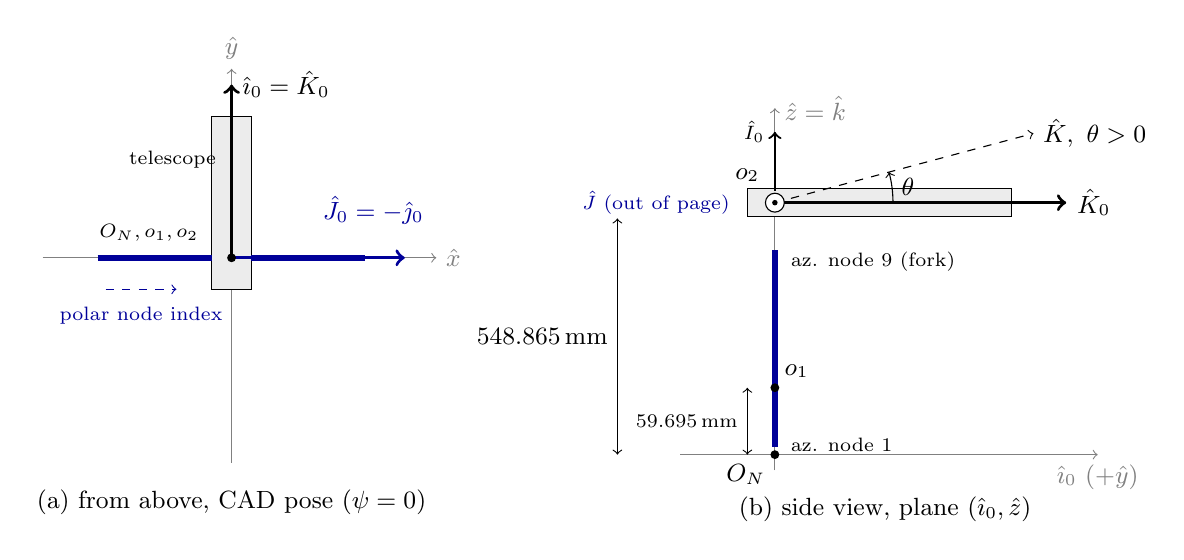
\begin{tikzpicture}[font=\small]
\begin{scope}
\draw[->, gray] (-2.4,0) -- (2.6,0) node[right] {$\hat x$};
\draw[->, gray] (0,-2.6) -- (0,2.4) node[above] {$\hat y$};
\draw[fill=gray!15] (-0.250,-0.400) -- (-0.250,1.800) -- (0.250,1.800) -- (0.250,-0.400) -- cycle;
\node[font=\scriptsize] at (-0.750,1.250) {telescope};
\draw[line width=2.2pt, blue!60!black] (-1.700,0.000) -- (-0.250,0.000);
\draw[line width=2.2pt, blue!60!black] (0.250,0.000) -- (1.700,0.000);
\draw[very thick, ->] (0,0) -- (0.000,2.200) node[anchor=west] {$\hat\imath_0 = \hat K_0$};
\draw[very thick, ->, blue!60!black] (0,0) -- (2.200,0.000);
\node[blue!60!black, anchor=south] at (1.800,0.300) {$\hat J_0 = -\hat\jmath_0$};
\draw[->, blue!60!black, dashed] (-1.600,-0.400) -- ++(-0.000:0.9);
\node[blue!60!black, font=\scriptsize, anchor=north] at (-1.150,-0.500) {polar node index};
\fill (0,0) circle (1.6pt);
\node[anchor=south east, font=\scriptsize] at (-0.300,0.080) {$O_N, o_1, o_2$};
\node at (0,-3.1) {(a) from above, CAD pose ($\psi = 0$)};
\end{scope}
\begin{scope}[xshift=6.9cm, yshift=-2.5cm]
\draw[->, gray] (-1.2,0) -- (4.1,0) node[below] {$\hat\imath_0$ $(+\hat{y})$};
\draw[->, gray] (0,-0.2) -- (0,4.4) node[right] {$\hat z = \hat k$};
\fill (0,0) circle (1.6pt) node[below left] {$O_N$};
\draw[line width=2.2pt, blue!60!black] (0,0.1) -- (0,2.600);
\fill (0.000,0.850) circle (1.6pt) node[above right] {$o_1$};
\node[right, font=\scriptsize] at (0.08,2.450) {az. node 9 (fork)};
\node[right, font=\scriptsize] at (0.08,0.12) {az. node 1};
\draw[fill=gray!15, rotate around={-0.000:(0,3.2)}] (-0.35,3.02) rectangle (3.0,3.3800000000000003);
\draw[very thick, ->, rotate around={-0.000:(0,3.2)}] (0,3.2) -- (3.7,3.2) node[right] {$\hat K_0$};
\draw[dashed, ->] (0,3.2) -- ++(15:3.4) node[right] {$\hat K,\ \theta>0$};
\draw[thick, ->] (0,3.2) ++(0.0,0.15) -- ++(0,0.75) node[left, font=\scriptsize] {$\hat I_0$};
\draw[->] (1.5,3.2) arc (0:15:1.5) node[midway, right] {$\theta$};
\draw[fill=white] (0,3.2) circle (0.12); \fill (0,3.2) circle (0.035);
\node at (-0.35,3.5500000000000003) {$o_2$};
\node[blue!60!black, font=\scriptsize, anchor=east] at (-0.45,3.2) {$\hat J$ (out of page)};
\draw[<->] (-2.0,0) -- (-2.0,3.0) node[midway, left] {$548.865$\,mm};
\draw[<->] (-0.35,0) -- (-0.35,0.850) node[midway, left, font=\scriptsize] {$59.695$\,mm};
\node at (1.4,-0.7) {(b) side view, plane $(\hat\imath_0, \hat z)$};
\end{scope}
\end{tikzpicture}}
\caption{CAD pose of the mount, drawn from the data of \texttt{frames}. (a) View from above: telescope along $\hat\imath_0 = \hat K_0$, polar shaft along $\hat J_0 = -\hat\jmath_0$ (blue) with the direction of increasing polar node index; $O_N$, $o_1$, $o_2$ project onto the same point. (b) Side view in the vertical plane of the pointing direction: origins $O_N$, $o_1$, $o_2$ on $\hat z$, azimuth shaft from node 1 to node 9 (fork), $\hat I_0$ upwards, $\hat J$ out of the page, $\theta>0$ raising the pointing.}\label{fig:frames}
\end{figure}
\subsection{Eccentricities}\label{subsec:eccentricity}
Because the body origins are on the rotation axes, the centre of mass of each body has an eccentricity with respect to its centre of rotation:
\begin{gather}
\mathbf e_1 = \mathbf r_{G_1} - \mathbf r_{o_1}\ \text{(fork, in frame 1)}, \qquad \mathbf d_2 = \mathbf R_{N2}^{(0)\mathsf T}\bigl(\mathbf r_{G_2} - \mathbf r_{o_2}\bigr)\ \text{(telescope, in frame 2)}.
\end{gather}
$\mathbf d_2$ enters the dynamics through the tensor $\mathbf I_{p,o_2}|_2$ (Huygens--Steiner) and the gravitational energy $m_p g\,(d_K\sin\theta_p + d_I\cos\theta_p)$ (height of $G_2$ above $o_2$); $d_J$ lies along the polar axis and never changes the height of the centre of mass. The fork turns only about $\hat k$, so in the current model its eccentricity enters only through its moment of inertia about the azimuth axis, $J_1 = I_{kk,G_1} + m_1\,(e_{1,x}^2 + e_{1,y}^2)$; keeping $o_1$ on the axis prepares the extension in which $\mathbf e_1$ acts explicitly.
\subsection{Coordinates along the shafts}
\begin{itemize}
\item \textbf{Azimuth shaft:} along $\hat k = \hat z$, node index increasing upwards (node 1 encoder at the bottom, node 9 fork at the top). $\psi_i$ is the absolute rotation of node $i$ about $\hat k$. The azimuth shaft turns only about its own axis, so only the axial inertias of its parts enter.
\item \textbf{Polar shaft:} along $\hat J = -\hat\jmath$. $\theta_i$ is the rotation of node $i$ about $\hat J$ relative to body 1, which is also its absolute rotation about $\hat J$. The polar node index increases along $+\hat J$ (\texttt{nodes\_increase\_along}), so the centre of mass of a polar piece at abscissa $x$ from node 1 sits at
\begin{gather}
y_c = y_1 + s\,x, \qquad s = +1,
\end{gather}
from $o_2$ along $\hat J$, where $y_1$ is \texttt{y\_node1\_from\_o2\_mm}. Currently $y_1$ is not given (\texttt{null}, Q7): the code then sets $y_c = 0$ for every piece, i.e.\ no Steiner term in $J^{ax}$. $y_c$ enters only $J^{ax}$ (Section~\ref{sec:coupled}).
\item \textbf{Telescope (hub model):} element 3 has no shaft; its nodes coincide with the hub centre H, and the telescope is the node P joined to H by the attachment spring $k_b$ (Section~\ref{sec:hub}); only the telescope inertia (\texttt{payload}) is attached to P.
\item \textbf{Element data} (\texttt{mode: manual}): $J$ about the shaft's own axis; $I_t$ about a transverse axis through the element's own centre of mass; \texttt{y\_c\_mm} measured from node $i$ in the direction of increasing node index.
\end{itemize}
\subsection{In which frame each inertia is entered}\label{subsec:input_frames}
\paragraph{Telescope (\texttt{payload}).} The dynamics needs the tensor of the telescope about $o_2$ in frame 2, $\mathbf I_{p,o_2}|_2$, with components $I_{II}, I_{JJ}, I_{KK}, I_{IJ}, I_{IK}, I_{JK}$ along $\hat I, \hat J, \hat K$, the mass $m_p$ and the eccentricity $\mathbf d_2 = [d_I, d_J, d_K]$. All tensors are in tensor convention, $I_{ab} = -\int a\,b\,dm$ for $a\neq b$. Two input frames are accepted (key \texttt{frame}):
\begin{enumerate}
\item \texttt{frame: cad\_cg} (recommended). Enter the tensor \emph{exactly as Onshape exports it with no mate connector selected}: about the centre of mass $G_2$ of the telescope, with axes parallel to $\hat x, \hat y, \hat z$ (\texttt{I\_kgm2}, kg\,m$^2$), and the centre of mass $\mathbf r_{G_2}|_N$ measured from $O_N$ (\texttt{r\_G\_mm}, mm). The code applies the sign convention (\texttt{products\_sign}), then
\begin{gather}
\mathbf r = \mathbf r_{G_2} - \mathbf r_{o_2}, \qquad\mathbf I_{p,o_2}|_N = \mathbf I_{p,G_2}|_N + m_p\left(\|\mathbf r\|^2\mathbf I - \mathbf r\,\mathbf r^{\mathsf T}\right), \\\mathbf I_{p,o_2}|_2 = \mathbf R_{N2}^{(0)\mathsf T}\,\mathbf I_{p,o_2}|_N\,\mathbf R_{N2}^{(0)}, \qquad \mathbf d_2 = \mathbf R_{N2}^{(0)\mathsf T}\,\mathbf r .
\end{gather}
With the current CAD pose this amounts to (components of $\mathbf I_{p,o_2}|_N$ on the right, $\Delta x, \Delta y, \Delta z$ the components of $\mathbf r$ in $N$):
\begin{gather}
I_{II} = I^{N}_{zz},\quad I_{JJ} = I^{N}_{xx},\quad I_{KK} = I^{N}_{yy}, \\
I_{IJ} = I^{N}_{xz},\quad I_{IK} = I^{N}_{yz},\quad I_{JK} = I^{N}_{xy}, \\
d_I = \Delta{z},\quad d_J = \Delta{x},\quad d_K = \Delta{y}.
\end{gather}
\item \texttt{frame: body2\_o2}. Enter $\mathbf I_{p,o_2}|_2$ directly (about $o_2$, axes $\hat I, \hat J, \hat K$) and $\mathbf d_2$ in mm (\texttt{d\_mm}); no transformation is applied.
\end{enumerate}
Checklist for an Onshape export with \texttt{frame: cad\_cg}:
\begin{itemize}
\item select only the telescope (there is no shaft through it) and keep \texttt{subtract\_shaft\_parts: false};
\item select no mate connector, so that the tensor is about the centre of mass with axes parallel to $\hat x, \hat y, \hat z$, and the centre of mass is measured from $O_N$;
\item export in the CAD pose of \texttt{frames}: telescope pointing along $+\hat{y}$ at $\theta_{cad} = 0^\circ$; if the assembly is in another pose, update \texttt{pointing\_cad}, \texttt{polar\_axis\_cad} and \texttt{theta\_cad\_deg};
\item convert to kg\,m$^2$ and mm, and set \texttt{products\_sign} (\texttt{tensor} if the off-diagonal terms are $-\int a\,b\,dm$, \texttt{positive} if they are $+\int a\,b\,dm$).
\end{itemize}
The code then checks that the tensor is symmetric, positive definite and satisfies the triangle inequality, and warns (\texttt{PAYLOAD\_ASSE\_SOSPETTO}) if the smallest centroidal moment is not about $\hat K$: for an optical tube this usually reveals a wrong pose or a wrong frame. Current input: \texttt{source: manual}, \texttt{frame: cad\_cg}, \texttt{subtract\_shaft\_parts: false}.
\paragraph{Current telescope data.}
As entered in \texttt{config.yaml} (Onshape, Telescopio LAMERA <1>, without mate connector):
\begin{gather}\mathbf I_{p,G_2}\big|_N = \begin{bmatrix}0.805643 & -1.679\times10^{-6} & 7.51\times10^{-7} \\ -1.679\times10^{-6} & 0.284157 & -0.0128698 \\ 7.51\times10^{-7} & -0.0128698 & 0.797637\end{bmatrix}\ \text{kg\,m}^2, \\ m = 16.61\ \text{kg}, \qquad \mathbf r_{G_2}\big|_N = [-0.0004821,\ 67.392,\ 544.07]\ \text{mm}.\end{gather}
Values used by the dynamics: $m_p = 16.61$\,kg, eccentricity $\mathbf d_2 = [-4.79,\ -0.0004821,\ 67.39]$\,mm (components along $\hat I, \hat J, \hat K$),
\begin{gather}\mathbf I_{p,o_2}\big|_2 = \begin{bmatrix}0.87307 & 7.1264\times10^{-7} & -0.0075079 \\ 7.1264\times10^{-7} & 0.88146 & -1.1393\times10^{-6} \\ -0.0075079 & -1.1393\times10^{-6} & 0.28454\end{bmatrix}\ \text{kg\,m}^2 .\end{gather}
\paragraph{Fork (body 1, azimuth node 9).} A scalar: the moment of inertia of the fork alone about the azimuth axis $\hat k$. From an export about the centre of mass with axes parallel to $N$, $J_1 = I_{zz,G_1} + m_1\,(x_{G_1}^2 + y_{G_1}^2)$ (the azimuth axis passes through $O_N$, so the horizontal components of $\mathbf r_{G_1}$ are those of the eccentricity $\mathbf e_1$).
\paragraph{Rotors and other node inertias.} $J$ about the axis of the shaft they sit on; for the polar axis also $m$ and the transverse $I_t$ about their own centre of mass, located at the node.
\section{Input geometry}\label{sec:geometry}
The figures are generated from \texttt{config.yaml}. Each segment is drawn as a rectangle whose width is proportional to its length and whose height is proportional to its outer diameter; the bore of hollow cylinders is hatched, torque-carrying steel layers are blue, aluminium light blue and non-carrying layers (spacers) orange; elements given as CAD data (\texttt{mode: manual}) are cross-hatched. Dimensions are in mm.
\begin{figure}[H]\centering
\resizebox{\linewidth}{!}{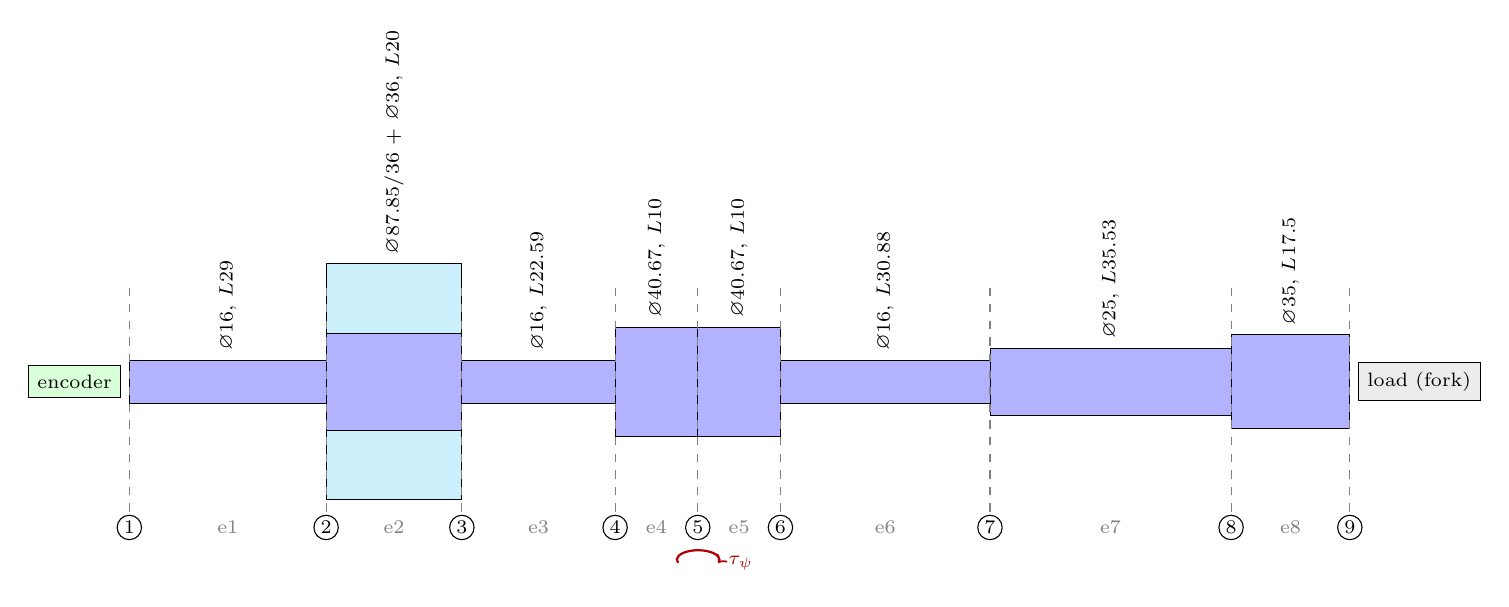
\begin{tikzpicture}[font=\scriptsize]
\filldraw[fill=blue!30, draw=black, line width=0.3pt] (0.000,-0.273) rectangle (2.499,0.273);
\node[rotate=90, anchor=west, inner sep=1pt] at (1.250,0.353) {$\varnothing16$, $L29$};
\filldraw[fill=cyan!20, draw=black, line width=0.3pt] (2.499,0.615) rectangle (4.223,1.500);
\filldraw[fill=cyan!20, draw=black, line width=0.3pt] (2.499,-1.500) rectangle (4.223,-0.615);
\filldraw[fill=blue!30, draw=black, line width=0.3pt] (2.499,-0.615) rectangle (4.223,0.615);
\node[rotate=90, anchor=west, inner sep=1pt] at (3.361,1.580) {$\varnothing87.85/36$ + $\varnothing36$, $L20$};
\filldraw[fill=blue!30, draw=black, line width=0.3pt] (4.223,-0.273) rectangle (6.169,0.273);
\node[rotate=90, anchor=west, inner sep=1pt] at (5.196,0.353) {$\varnothing16$, $L22.59$};
\filldraw[fill=blue!30, draw=black, line width=0.3pt] (6.169,-0.694) rectangle (7.219,0.694);
\node[rotate=90, anchor=west, inner sep=1pt] at (6.694,0.774) {$\varnothing40.67$, $L10$};
\filldraw[fill=blue!30, draw=black, line width=0.3pt] (7.219,-0.694) rectangle (8.269,0.694);
\node[rotate=90, anchor=west, inner sep=1pt] at (7.744,0.774) {$\varnothing40.67$, $L10$};
\filldraw[fill=blue!30, draw=black, line width=0.3pt] (8.269,-0.273) rectangle (10.930,0.273);
\node[rotate=90, anchor=west, inner sep=1pt] at (9.600,0.353) {$\varnothing16$, $L30.88$};
\filldraw[fill=blue!30, draw=black, line width=0.3pt] (10.930,-0.427) rectangle (13.992,0.427);
\node[rotate=90, anchor=west, inner sep=1pt] at (12.461,0.507) {$\varnothing25$, $L35.53$};
\filldraw[fill=blue!30, draw=black, line width=0.3pt] (13.992,-0.598) rectangle (15.500,0.598);
\node[rotate=90, anchor=west, inner sep=1pt] at (14.746,0.678) {$\varnothing35$, $L17.5$};
\draw[dashed, gray] (0.000,-1.650) -- (0.000,1.250);
\node[circle, draw, inner sep=1pt] at (0.000,-1.850) {1};
\draw[dashed, gray] (2.499,-1.650) -- (2.499,1.250);
\node[circle, draw, inner sep=1pt] at (2.499,-1.850) {2};
\draw[dashed, gray] (4.223,-1.650) -- (4.223,1.250);
\node[circle, draw, inner sep=1pt] at (4.223,-1.850) {3};
\draw[dashed, gray] (6.169,-1.650) -- (6.169,1.250);
\node[circle, draw, inner sep=1pt] at (6.169,-1.850) {4};
\draw[dashed, gray] (7.219,-1.650) -- (7.219,1.250);
\node[circle, draw, inner sep=1pt] at (7.219,-1.850) {5};
\draw[dashed, gray] (8.269,-1.650) -- (8.269,1.250);
\node[circle, draw, inner sep=1pt] at (8.269,-1.850) {6};
\draw[dashed, gray] (10.930,-1.650) -- (10.930,1.250);
\node[circle, draw, inner sep=1pt] at (10.930,-1.850) {7};
\draw[dashed, gray] (13.992,-1.650) -- (13.992,1.250);
\node[circle, draw, inner sep=1pt] at (13.992,-1.850) {8};
\draw[dashed, gray] (15.500,-1.650) -- (15.500,1.250);
\node[circle, draw, inner sep=1pt] at (15.500,-1.850) {9};
\node[gray] at (1.250,-1.850) {e1};
\node[gray] at (3.361,-1.850) {e2};
\node[gray] at (5.196,-1.850) {e3};
\node[gray] at (6.694,-1.850) {e4};
\node[gray] at (7.744,-1.850) {e5};
\node[gray] at (9.600,-1.850) {e6};
\node[gray] at (12.461,-1.850) {e7};
\node[gray] at (14.746,-1.850) {e8};
\draw[->, thick, red!70!black] (6.969,-2.300) arc[start angle=200, end angle=-20, x radius=0.27, y radius=0.12] node[right] {$\tau_\psi$};
\node[draw, fill=green!15, anchor=east] at (-0.100,0) {encoder};
\node[draw, fill=gray!15, anchor=west] at (15.600,0) {load (fork)};
\end{tikzpicture}}
\caption{Azimuth shaft as entered in \texttt{config.yaml} (drawn horizontally; node 1 is at the bottom). Elements shorter than the readable minimum are stretched: lengths are to scale within each element, not across elements. Vertical scale: proportional to the diameter.}
\label{fig:geom_azimut}\end{figure}
\begin{figure}[H]\centering
\resizebox{\linewidth}{!}{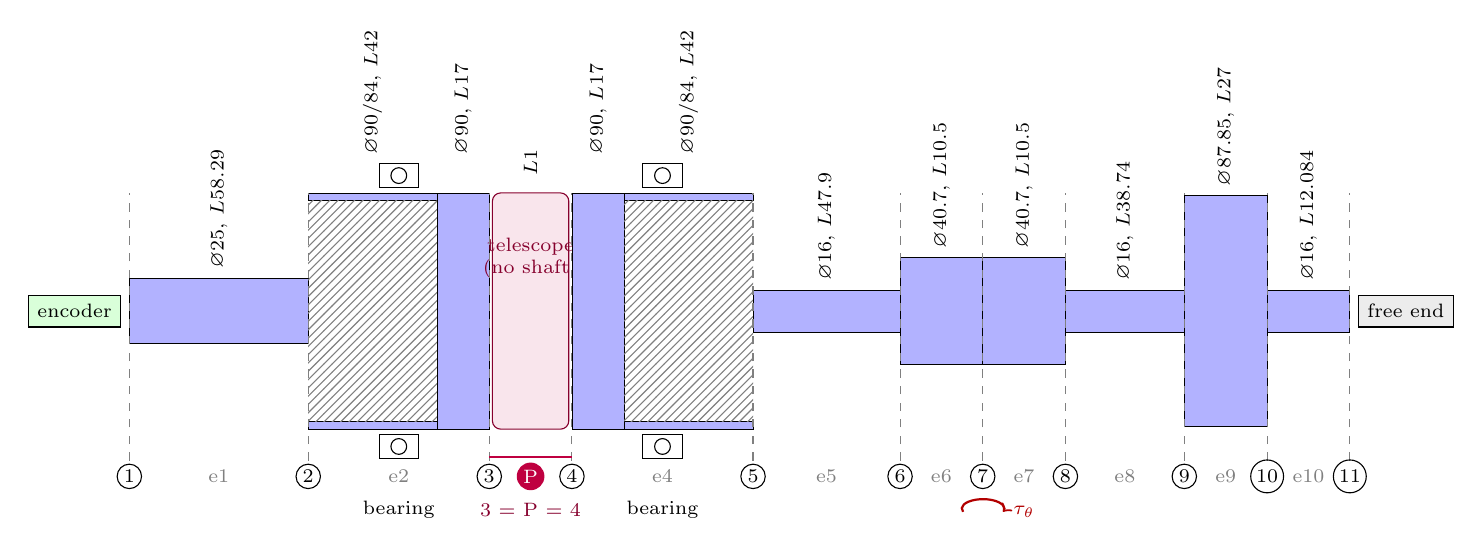
\begin{tikzpicture}[font=\scriptsize]
\filldraw[fill=blue!30, draw=black, line width=0.3pt] (0.000,-0.417) rectangle (2.272,0.417);
\node[rotate=90, anchor=west, inner sep=1pt] at (1.136,0.497) {$\varnothing25$, $L58.29$};
\filldraw[fill=blue!30, draw=black, line width=0.3pt] (2.272,1.400) rectangle (3.909,1.500);
\filldraw[fill=blue!30, draw=black, line width=0.3pt] (2.272,-1.500) rectangle (3.909,-1.400);
\fill[pattern=north east lines, pattern color=gray] (2.272,-1.400) rectangle (3.909,1.400);
\node[rotate=90, anchor=west, inner sep=1pt] at (3.090,1.950) {$\varnothing90/84$, $L42$};
\filldraw[fill=blue!30, draw=black, line width=0.3pt] (3.909,-1.500) rectangle (4.571,1.500);
\node[rotate=90, anchor=west, inner sep=1pt] at (4.240,1.950) {$\varnothing90$, $L17$};
\draw[rounded corners=3pt, fill=purple!10, draw=purple!70!black] (4.611,-1.500) rectangle (5.581,1.500);
\node[purple!70!black, align=center, font=\scriptsize] at (5.096,0.675) {telescope\\(no shaft)};
\node[rotate=90, anchor=west] at (5.096,1.600) {$L1$};
\filldraw[fill=blue!30, draw=black, line width=0.3pt] (5.621,-1.500) rectangle (6.284,1.500);
\node[rotate=90, anchor=west, inner sep=1pt] at (5.953,1.950) {$\varnothing90$, $L17$};
\filldraw[fill=blue!30, draw=black, line width=0.3pt] (6.284,1.400) rectangle (7.921,1.500);
\filldraw[fill=blue!30, draw=black, line width=0.3pt] (6.284,-1.500) rectangle (7.921,-1.400);
\fill[pattern=north east lines, pattern color=gray] (6.284,-1.400) rectangle (7.921,1.400);
\node[rotate=90, anchor=west, inner sep=1pt] at (7.102,1.950) {$\varnothing90/84$, $L42$};
\filldraw[fill=blue!30, draw=black, line width=0.3pt] (7.921,-0.267) rectangle (9.788,0.267);
\node[rotate=90, anchor=west, inner sep=1pt] at (8.854,0.347) {$\varnothing16$, $L47.9$};
\filldraw[fill=blue!30, draw=black, line width=0.3pt] (9.788,-0.678) rectangle (10.838,0.678);
\node[rotate=90, anchor=west, inner sep=1pt] at (10.313,0.758) {$\varnothing40.7$, $L10.5$};
\filldraw[fill=blue!30, draw=black, line width=0.3pt] (10.838,-0.678) rectangle (11.888,0.678);
\node[rotate=90, anchor=west, inner sep=1pt] at (11.363,0.758) {$\varnothing40.7$, $L10.5$};
\filldraw[fill=blue!30, draw=black, line width=0.3pt] (11.888,-0.267) rectangle (13.398,0.267);
\node[rotate=90, anchor=west, inner sep=1pt] at (12.643,0.347) {$\varnothing16$, $L38.74$};
\filldraw[fill=blue!30, draw=black, line width=0.3pt] (13.398,-1.464) rectangle (14.450,1.464);
\node[rotate=90, anchor=west, inner sep=1pt] at (13.924,1.544) {$\varnothing87.85$, $L27$};
\filldraw[fill=blue!30, draw=black, line width=0.3pt] (14.450,-0.267) rectangle (15.500,0.267);
\node[rotate=90, anchor=west, inner sep=1pt] at (14.975,0.347) {$\varnothing16$, $L12.084$};
\draw[dashed, gray] (0.000,-1.900) -- (0.000,1.500);
\node[circle, draw, inner sep=1pt] at (0.000,-2.100) {1};
\draw[dashed, gray] (2.272,-1.900) -- (2.272,1.500);
\node[circle, draw, inner sep=1pt] at (2.272,-2.100) {2};
\draw[dashed, gray] (4.571,-1.900) -- (4.571,1.500);
\node[circle, draw, inner sep=1pt] at (4.571,-2.100) {3};
\draw[dashed, gray] (5.621,-1.900) -- (5.621,1.500);
\node[circle, draw, inner sep=1pt] at (5.621,-2.100) {4};
\draw[dashed, gray] (7.921,-1.900) -- (7.921,1.500);
\node[circle, draw, inner sep=1pt] at (7.921,-2.100) {5};
\draw[dashed, gray] (9.788,-1.900) -- (9.788,1.500);
\node[circle, draw, inner sep=1pt] at (9.788,-2.100) {6};
\draw[dashed, gray] (10.838,-1.900) -- (10.838,1.500);
\node[circle, draw, inner sep=1pt] at (10.838,-2.100) {7};
\draw[dashed, gray] (11.888,-1.900) -- (11.888,1.500);
\node[circle, draw, inner sep=1pt] at (11.888,-2.100) {8};
\draw[dashed, gray] (13.398,-1.900) -- (13.398,1.500);
\node[circle, draw, inner sep=1pt] at (13.398,-2.100) {9};
\draw[dashed, gray] (14.450,-1.900) -- (14.450,1.500);
\node[circle, draw, inner sep=1pt] at (14.450,-2.100) {10};
\draw[dashed, gray] (15.500,-1.900) -- (15.500,1.500);
\node[circle, draw, inner sep=1pt] at (15.500,-2.100) {11};
\node[gray] at (1.136,-2.100) {e1};
\node[gray] at (3.422,-2.100) {e2};
\node[gray] at (5.096,-2.100) {e3};
\node[gray] at (6.771,-2.100) {e4};
\node[gray] at (8.854,-2.100) {e5};
\node[gray] at (10.313,-2.100) {e6};
\node[gray] at (11.363,-2.100) {e7};
\node[gray] at (12.643,-2.100) {e8};
\node[gray] at (13.924,-2.100) {e9};
\node[gray] at (14.975,-2.100) {e10};
\draw[->, thick, red!70!black] (10.588,-2.550) arc[start angle=200, end angle=-20, x radius=0.27, y radius=0.12] node[right] {$\tau_\theta$};
\node[draw, fill=green!15, anchor=east] at (-0.100,0) {encoder};
\node[draw, fill=gray!15, anchor=west] at (15.600,0) {free end};
\draw[fill=white] (3.172,1.570) rectangle (3.672,1.870);
\draw (3.422,1.720) circle (0.1);
\draw[fill=white] (3.172,-1.870) rectangle (3.672,-1.570);
\draw (3.422,-1.720) circle (0.1);
\node[font=\scriptsize] at (3.422,-2.520) {bearing};
\draw[fill=white] (6.521,1.570) rectangle (7.021,1.870);
\draw (6.771,1.720) circle (0.1);
\draw[fill=white] (6.521,-1.870) rectangle (7.021,-1.570);
\draw (6.771,-1.720) circle (0.1);
\node[font=\scriptsize] at (6.771,-2.520) {bearing};
\draw[thick, purple] (4.571,-1.850) -- (5.621,-1.850);
\node[purple!70!black, font=\scriptsize] at (5.096,-2.520) {3 = P = 4};
\node[circle, fill=purple, text=white, inner sep=1pt] at (5.096,-2.100) {P};
\end{tikzpicture}}
\caption{Polar shaft as entered in \texttt{config.yaml}; elements 2 and 4 are the side hubs (tube and flange) and element 3 has no shaft: its nodes coincide with the hub centre H, from which the telescope hangs through $k_b$ (the support ring is in Figure~\ref{fig:hub_geometry}). Elements shorter than the readable minimum are stretched: lengths are to scale within each element, not across elements. Vertical scale: proportional to the diameter.}
\label{fig:geom_polare}\end{figure}
\section{Element properties}\label{sec:elements}
For an annular layer of length $L$, outer and inner diameters $D_o$, $D_i$ ($D_i = 0$ for a solid cylinder), density $\rho$ and shear modulus $G$:
\begin{gather}
m = \rho\,\frac{\pi}{4}\left(D_o^2 - D_i^2\right)L, \qquad
J = \frac{\pi\rho L}{32}\left(D_o^4 - D_i^4\right) = \frac{m}{8}\left(D_o^2 + D_i^2\right), \\
I_t = m\left[\frac{D_o^2 + D_i^2}{16} + \frac{L^2}{12}\right], \qquad
J_p = \frac{\pi}{32}\left(D_o^4 - D_i^4\right).
\end{gather}
$J$ is the axial mass moment of inertia, $I_t$ the transverse one about the layer's own centre of mass and $J_p$ the polar second moment of area. Coaxial layers of a segment add their masses and inertias, and the torque-carrying layers act in parallel; the segments of an element add their inertias and act in series, together with an optional joint compliance:
\begin{gather}
k_s = \frac{1}{L_s}\sum_{\ell\ \text{carrying}} G_\ell J_{p,\ell}, \qquad
\frac{1}{k_e} = \sum_s \frac{1}{k_s} + \frac{1}{k_{joint}}, \qquad
J_e = \sum_s\sum_\ell J_{s\ell} + \sum J^{x}_e.
\end{gather}
$J^{x}_e$ are concentrated extra inertias attached to the element. An element given as CAD data enters with its $J_e$ and $k_e$ directly. The transverse inertia of the element about its own centre of mass follows from the layers by the parallel-axis theorem along the shaft.
\begingroup\footnotesize\setlength{\tabcolsep}{3.2pt}
\begin{longtable}{llllrrrlcrrrr}
\caption{Element properties, azimuth axis: layer contributions and element totals ($m$ in g, inertias in kg\,m$^2$, $k$ in N\,m/rad).}\\
\toprule
el. & seg. & lay. & shape & $D_o$ & $D_i$ & $L$ & mat. & carr. & $m$ & $J$ & $I_t$ & $k$ \\
\midrule\endfirsthead
\toprule el. & seg. & lay. & shape & $D_o$ & $D_i$ & $L$ & mat. & carr. & $m$ & $J$ & $I_t$ & $k$ \\ \midrule\endhead
1 & 1 & 1 & solid & 16 & 0 & 29 & steel & yes & $46.6$ & $1.49\times10^{-6}$ & $4.02\times10^{-6}$ & $1.71\times10^{4}$ \\
\midrule \textbf{1} & \multicolumn{5}{l}{total (geometry)} & 29 & & & $46.65$ & $1.493\times10^{-6}$ & $4.015\times10^{-6}$ & $1.708\times10^{4}$ \\ \midrule
2 & 1 & 1 & solid & 36 & 0 & 20 & steel & yes & $163$ & $2.64\times10^{-5}$ & $1.86\times10^{-5}$ & $6.35\times10^{5}$ \\
2 & 1 & 2 & hollow & 87.85 & 36 & 20 & aluminium & yes & $283$ & $0.000319$ & $0.000169$ & $7.64\times10^{6}$ \\
\midrule \textbf{2} & \multicolumn{5}{l}{total (geometry)} & 20 & & & $446.3$ & $0.0003457$ & $0.0001877$ & $8.278\times10^{6}$ \\ \midrule
3 & 1 & 1 & solid & 16 & 0 & 22.59 & steel & yes & $36.3$ & $1.16\times10^{-6}$ & $2.13\times10^{-6}$ & $2.19\times10^{4}$ \\
\midrule \textbf{3} & \multicolumn{5}{l}{total (geometry)} & 22.59 & & & $36.34$ & $1.163\times10^{-6}$ & $2.127\times10^{-6}$ & $2.193\times10^{4}$ \\ \midrule
4 & 1 & 1 & solid & 40.67 & 0 & 10 & steel & yes & $104$ & $2.15\times10^{-5}$ & $1.16\times10^{-5}$ & $2.07\times10^{6}$ \\
\midrule \textbf{4} & \multicolumn{5}{l}{total (geometry)} & 10 & & & $103.9$ & $2.149\times10^{-5}$ & $1.161\times10^{-5}$ & $2.068\times10^{6}$ \\ \midrule
5 & 1 & 1 & solid & 40.67 & 0 & 10 & steel & yes & $104$ & $2.15\times10^{-5}$ & $1.16\times10^{-5}$ & $2.07\times10^{6}$ \\
\midrule \textbf{5} & \multicolumn{5}{l}{total (geometry)} & 10 & & & $103.9$ & $2.149\times10^{-5}$ & $1.161\times10^{-5}$ & $2.068\times10^{6}$ \\ \midrule
6 & 1 & 1 & solid & 16 & 0 & 30.88 & steel & yes & $49.7$ & $1.59\times10^{-6}$ & $4.74\times10^{-6}$ & $1.6\times10^{4}$ \\
\midrule \textbf{6} & \multicolumn{5}{l}{total (geometry)} & 30.88 & & & $49.67$ & $1.589\times10^{-6}$ & $4.742\times10^{-6}$ & $1.604\times10^{4}$ \\ \midrule
7 & 1 & 1 & solid & 25 & 0 & 35.53 & steel & yes & $140$ & $1.09\times10^{-5}$ & $2.01\times10^{-5}$ & $8.31\times10^{4}$ \\
\midrule \textbf{7} & \multicolumn{5}{l}{total (geometry)} & 35.53 & & & $139.5$ & $1.09\times10^{-5}$ & $2.013\times10^{-5}$ & $8.311\times10^{4}$ \\ \midrule
8 & 1 & 1 & solid & 35 & 0 & 17.5 & steel & yes & $135$ & $2.06\times10^{-5}$ & $1.38\times10^{-5}$ & $6.48\times10^{5}$ \\
\midrule \textbf{8} & \multicolumn{5}{l}{total (geometry)} & 17.5 & & & $134.7$ & $2.063\times10^{-5}$ & $1.375\times10^{-5}$ & $6.482\times10^{5}$ \\ \midrule
\bottomrule\end{longtable}
\endgroup
\begingroup\footnotesize\setlength{\tabcolsep}{3.2pt}
\begin{longtable}{llllrrrlcrrrr}
\caption{Element properties, polar axis: layer contributions and element totals ($m$ in g, inertias in kg\,m$^2$, $k$ in N\,m/rad).}\\
\toprule
el. & seg. & lay. & shape & $D_o$ & $D_i$ & $L$ & mat. & carr. & $m$ & $J$ & $I_t$ & $k$ \\
\midrule\endfirsthead
\toprule el. & seg. & lay. & shape & $D_o$ & $D_i$ & $L$ & mat. & carr. & $m$ & $J$ & $I_t$ & $k$ \\ \midrule\endhead
1 & 1 & 1 & solid & 25 & 0 & 58.29 & steel & yes & $229$ & $1.79\times10^{-5}$ & $7.38\times10^{-5}$ & $5.07\times10^{4}$ \\
\midrule \textbf{1} & \multicolumn{5}{l}{total (geometry)} & 58.29 & & & $228.9$ & $1.788\times10^{-5}$ & $7.375\times10^{-5}$ & $5.066\times10^{4}$ \\ \midrule
\midrule \textbf{2} & \multicolumn{5}{l}{total (hub)} & 214 & & & $0$ & $0$ & $0$ & $1805$ \\ \midrule
\midrule \textbf{3} & \multicolumn{5}{l}{total (telescope)} & 1 & & & $0$ & $0$ & $0$ & $--$ \\ \midrule
\midrule \textbf{4} & \multicolumn{5}{l}{total (hub)} & 214 & & & $0$ & $0$ & $0$ & $1805$ \\ \midrule
5 & 1 & 1 & solid & 16 & 0 & 47.9 & steel & yes & $77$ & $2.47\times10^{-6}$ & $1.6\times10^{-5}$ & $1.03\times10^{4}$ \\
\midrule \textbf{5} & \multicolumn{5}{l}{total (geometry)} & 47.9 & & & $77.05$ & $2.466\times10^{-6}$ & $1.596\times10^{-5}$ & $1.034\times10^{4}$ \\ \midrule
6 & 1 & 1 & solid & 40.7 & 0 & 10.5 & steel & yes & $109$ & $2.26\times10^{-5}$ & $1.23\times10^{-5}$ & $1.98\times10^{6}$ \\
\midrule \textbf{6} & \multicolumn{5}{l}{total (geometry)} & 10.5 & & & $109.3$ & $2.263\times10^{-5}$ & $1.232\times10^{-5}$ & $1.976\times10^{6}$ \\ \midrule
7 & 1 & 1 & solid & 40.7 & 0 & 10.5 & steel & yes & $109$ & $2.26\times10^{-5}$ & $1.23\times10^{-5}$ & $1.98\times10^{6}$ \\
\midrule \textbf{7} & \multicolumn{5}{l}{total (geometry)} & 10.5 & & & $109.3$ & $2.263\times10^{-5}$ & $1.232\times10^{-5}$ & $1.976\times10^{6}$ \\ \midrule
8 & 1 & 1 & solid & 16 & 0 & 38.74 & steel & yes & $62.3$ & $1.99\times10^{-6}$ & $8.79\times10^{-6}$ & $1.28\times10^{4}$ \\
\midrule \textbf{8} & \multicolumn{5}{l}{total (geometry)} & 38.74 & & & $62.31$ & $1.994\times10^{-6}$ & $8.79\times10^{-6}$ & $1.279\times10^{4}$ \\ \midrule
9 & 1 & 1 & solid & 87.85 & 0 & 27 & steel & yes & $1.31\times10^{3}$ & $0.00126$ & $0.000711$ & $1.67\times10^{7}$ \\
\midrule \textbf{9} & \multicolumn{5}{l}{total (geometry)} & 27 & & & $1309$ & $0.001263$ & $0.0007111$ & $1.668\times10^{7}$ \\ \midrule
10 & 1 & 1 & solid & 16 & 0 & 12.084 & steel & yes & $19.4$ & $6.22\times10^{-7}$ & $5.48\times10^{-7}$ & $4.1\times10^{4}$ \\
\midrule \textbf{10} & \multicolumn{5}{l}{total (geometry)} & 12.084 & & & $19.44$ & $6.22\times10^{-7}$ & $5.475\times10^{-7}$ & $4.1\times10^{4}$ \\ \midrule
\bottomrule\end{longtable}
\endgroup
\section{Hub and compliant telescope attachment (hub model)}\label{sec:hub}
\paragraph{Purpose and switch.} This document is generated with \texttt{polar.hub.enabled: true} (file \texttt{config\_hub.yaml}, results in \texttt{results\_hub/}). The original model, with the telescope rigidly attached to the shaft node P, is kept in \texttt{config.yaml} and \texttt{results/}; the flag switches between the two. The hub model follows the antiresonance measured at the elevation encoder (Section~\ref{sec:experimental}): a zero at an encoder on the load side requires a large inertia outside the encoder--motor path, so the telescope is no longer rigid on the shaft but hangs from the hub through a compliance $k_b$.
\paragraph{Topology.} The two side hubs and the support ring form the hub, which carries the torque between the two polar bearings; its centre H (at $o_2$) carries the inertia of the hub. The two halves of the hub replace polar elements 2 and 4 as massless springs, element 3 (no shaft) collapses into H, and the telescope is a node P off the chain:
\begin{gather}
1 \overset{e_1}{\longleftrightarrow} 2 \overset{\text{half hub}}{\longleftrightarrow} \mathrm H \overset{\text{half hub}}{\longleftrightarrow} 5 \overset{e_5}{\longleftrightarrow} 6 \cdots 11, \qquad \mathrm H \overset{k_b}{\longleftrightarrow} \mathrm P\ (\text{telescope}).
\end{gather}
\paragraph{Geometry.} Each side hub is a single steel body: a solid flange fixed to the ring and a tube that seats the bearings. The support ring (aluminium) holds the telescope, which is slid into it, so its axis is the telescope axis $\hat K$, perpendicular to the polar axis; the side hubs are fixed to it at two diametrically opposite points. The materials follow from the mass: the nominal geometry gives $7.643\times10^{5}$\,mm$^3$ and $3.63$\,kg with an aluminium ring and steel side hubs, against $3.534$\,kg in Onshape.
\begin{figure}[H]\centering
\includegraphics[width=\linewidth,height=0.75\textheight,keepaspectratio]{../figures/geometria_mozzo.pdf}
\caption{Hub of the polar axis as used for the stiffness: (a) view from above, with the polar axis horizontal and the telescope (ring) axis vertical; (b) view along the telescope axis; (c) springs in series from bearing to bearing, with the telescope attached to the hub centre H through $k_b$. Dimensions in mm, stiffnesses in N\,m/rad. \emph{Result from placeholder parameters.}}\label{fig:hub_geometry}\end{figure}
\paragraph{Stiffness.} The parts are springs in series. The tube and the flange are shafts in torsion, $k = G J_p/L$. The ring, loaded by a couple $M$ about $\hat J$ at each attachment point, works as two half rings in parallel; along each half the moment is the constant vector $\tfrac12 M\hat J$, which splits into an out-of-plane bending moment $\tfrac12 M\cos\varphi$ about the radius and a torque $\tfrac12 M\sin\varphi$ about the tangent. The complementary energy (Castigliano) gives
\begin{gather}
\theta = \frac{\pi R}{4}\left(\frac{1}{E I_r} + \frac{1}{G J_t}\right) M,\qquad k_{ring} = \frac{4}{\pi R}\left(\frac{1}{E I_r} + \frac{1}{G J_t}\right)^{-1},\\
I_r = \frac{t\,b^3}{12},\qquad J_t = \beta\,b\,t^3,\quad \beta = \tfrac13\bigl(1 - 0.63\,\tfrac tb + 0.052\,(\tfrac tb)^5\bigr),\qquad E = 2G(1 + \nu),
\end{gather}
with the mean radius $R = 152.5$\,mm, the wall thickness $t = 5$\,mm, the width $b = 100$\,mm and $\nu = 0.33$: $E I_r = 2.98\times10^{4}$\,N\,m$^2$ and $G J_t = 109$\,N\,m$^2$. The thin wall twists easily, so the ring dominates the series. The ring is taken alone, without the stiffening of the telescope tube slid into it (user's choice): its value is a lower bound.
\begin{table}[H]\centering\small
\caption{Hub parts, geometry (mm) and torsional stiffness about the polar axis (N\,m/rad). \emph{Result from placeholder parameters.}}\label{tab:hub_parts}
\begin{tabular}{llr}\toprule
part & geometry & $k$ \\ \midrule
side hub: bearing-seat tube & 90/84 x 42, steel & $2.848\times10^{6}$ \\
side hub: flange & 90 x 17 (solid), steel & $2.918\times10^{7}$ \\
support ring (two half rings) & 310/300 x 100, aluminium & $903$ \\
\midrule
half hub (tube, flange, half ring: $2k_{ring}$) & in series & $1805$ \\
whole hub, bearing to bearing & in series & $902.4$ \\
telescope attachment $k_b$ & placeholder (see text) & $9800$ \\
\bottomrule\end{tabular}\end{table}
\paragraph{Inertia.} From the Onshape export of the three parts (Onshape: Ruota di trasmissione <1>, <2> + T-02 Anello di registrazione del telescopio <1>), mass $3.534$\,kg, centre of mass at $0$\,mm from $o_2$, tensor about the centre of mass in the axes of N (kg\,m$^2$)
\begin{gather}
\mathbf I_{hub,G}|_N = \begin{bmatrix}0.01881 & -1.5\times10^{-8} & 2\times10^{-9} \\ -1.5\times10^{-8} & 0.09604 & 2.438\times10^{-6} \\ 2\times10^{-9} & 2.438\times10^{-6} & 0.08237\end{bmatrix}.
\end{gather}
Transported to $o_2$ and rotated into the frame of body 2, it gives $J_{hub} = 0.01881$\,kg\,m$^2$ about the polar axis, at node H, and $0.08237$\,kg\,m$^2$ about $\hat z$ at $\theta = 0$, added to $J^{ax}$ because the azimuth load exported from Onshape does not contain the hub (\texttt{in\_azimuth\_load: false}).
\paragraph{Telescope attachment.} The spring $k_b$ joins H to the telescope node P, which carries only the telescope (payload section). Its value is not computed from a geometry: it is a placeholder, the two-mass estimate from the antiresonance and resonance measured at the elevation encoder. With the shafts, the reduced polar tree has $k_{\theta,1} = 1743$ (encoder--H), $k_{\theta,2} = 1535$ (H--motor), $k_{\theta,3} = 9694$ (motor--rear end) and $k_{\theta,4} = k_b = 9800$\,N\,m/rad (H--P).
\section{\texorpdfstring{Finite element model of each axis}{Finite element model of each axis}}\label{sec:fem}
\paragraph{Element matrices.} The two-node torsional element has
\begin{gather}
\mathbf K_e = k_e\begin{bmatrix}1&-1\\-1&1\end{bmatrix}, \qquad
\mathbf M_e^{\ell} = \frac{J_e}{2}\begin{bmatrix}1&0\\0&1\end{bmatrix} \quad\text{(lumped)}.
\end{gather}
For the consistent mass, the inertia per unit length $\bar J(x)$ is piecewise constant (one value $\bar J_s = J_s/L_s$ per segment) and the shape functions are linear, $N_1 = 1 - x/L_e$, $N_2 = x/L_e$:
\begin{gather}
(\mathbf M_e^{c})_{ab} = \sum_s \bar J_s\int_{x_s}^{x_s+L_s} N_a N_b\,dx
= \sum_s \bar J_s\,\frac{L_s}{6}\Bigl(2N_a^0N_b^0 + N_a^0N_b^1 + N_a^1N_b^0 + 2N_a^1N_b^1\Bigr)
+ \frac{J^{x}_e}{2}\,\mathbf I,
\end{gather}
where $N_a^0$, $N_a^1$ are the values of $N_a$ at the ends of segment $s$: the formula is exact because the integrand is the product of two linear functions on each segment. For one uniform segment it gives $\mathbf M_e^{c} = \frac{J_e}{6}\left[\begin{smallmatrix}2&1\\1&2\end{smallmatrix}\right]$. We write $a_e$, $b_e$, $c_e$ for the entries $(1,1)$, $(1,2)$, $(2,2)$ of $\mathbf M_e^{c}$.
\paragraph{Nodes H and P (hub model).} Element 3 has no shaft: its nodes 3 and 4 coincide with the hub centre H, which carries the hub inertia $J^n_H$. Elements 2 and 4 are the two halves of the hub, massless springs (their inertia is in $J^n_H$). The telescope node P is an extra node, last in the ordering, joined to H by the massless spring $k_b$: it carries no inertia of its own in $\mathbf M$, the telescope enters through the payload (Section~\ref{sec:hub}). The matrices are therefore those of a tree, not of a chain.
\paragraph{Assembly.} The global matrices are assembled by summing on the shared nodes; the concentrated inertias $J^{n}$ (rotors, fork) are added on the diagonal and the generalised force is $\mathbf Q = \tau\,\mathbf e_p$ with $p$ the motor node. In symbolic form:
\paragraph{Azimuth axis} (node order 1, 2, 3, 4, 5, 6, 7, 8, 9):
\begin{center}\resizebox{\linewidth}{!}{$\displaystyle \mathbf K = \left[\begin{matrix}k_{1} & - k_{1} & 0 & 0 & 0 & 0 & 0 & 0 & 0\\- k_{1} & k_{1} + k_{2} & - k_{2} & 0 & 0 & 0 & 0 & 0 & 0\\0 & - k_{2} & k_{2} + k_{3} & - k_{3} & 0 & 0 & 0 & 0 & 0\\0 & 0 & - k_{3} & k_{3} + k_{4} & - k_{4} & 0 & 0 & 0 & 0\\0 & 0 & 0 & - k_{4} & k_{4} + k_{5} & - k_{5} & 0 & 0 & 0\\0 & 0 & 0 & 0 & - k_{5} & k_{5} + k_{6} & - k_{6} & 0 & 0\\0 & 0 & 0 & 0 & 0 & - k_{6} & k_{6} + k_{7} & - k_{7} & 0\\0 & 0 & 0 & 0 & 0 & 0 & - k_{7} & k_{7} + k_{8} & - k_{8}\\0 & 0 & 0 & 0 & 0 & 0 & 0 & - k_{8} & k_{8}\end{matrix}\right]$}\end{center}
\begin{center}\resizebox{\linewidth}{!}{$\displaystyle \mathbf M^{\ell} = \left[\begin{matrix}\frac{J_{1}}{2} & 0 & 0 & 0 & 0 & 0 & 0 & 0 & 0\\0 & \frac{J_{1}}{2} + \frac{J_{2}}{2} & 0 & 0 & 0 & 0 & 0 & 0 & 0\\0 & 0 & \frac{J_{2}}{2} + \frac{J_{3}}{2} & 0 & 0 & 0 & 0 & 0 & 0\\0 & 0 & 0 & \frac{J_{3}}{2} + \frac{J_{4}}{2} & 0 & 0 & 0 & 0 & 0\\0 & 0 & 0 & 0 & \frac{J_{4}}{2} + \frac{J_{5}}{2} & 0 & 0 & 0 & 0\\0 & 0 & 0 & 0 & 0 & \frac{J_{5}}{2} + \frac{J_{6}}{2} & 0 & 0 & 0\\0 & 0 & 0 & 0 & 0 & 0 & \frac{J_{6}}{2} + \frac{J_{7}}{2} & 0 & 0\\0 & 0 & 0 & 0 & 0 & 0 & 0 & \frac{J_{7}}{2} + \frac{J_{8}}{2} & 0\\0 & 0 & 0 & 0 & 0 & 0 & 0 & 0 & J^{n}_{9} + \frac{J_{8}}{2}\end{matrix}\right]$}\end{center}
\begin{center}\resizebox{\linewidth}{!}{$\displaystyle \mathbf M^{c} = \left[\begin{matrix}a_{1} & b_{1} & 0 & 0 & 0 & 0 & 0 & 0 & 0\\b_{1} & a_{2} + c_{1} & b_{2} & 0 & 0 & 0 & 0 & 0 & 0\\0 & b_{2} & a_{3} + c_{2} & b_{3} & 0 & 0 & 0 & 0 & 0\\0 & 0 & b_{3} & a_{4} + c_{3} & b_{4} & 0 & 0 & 0 & 0\\0 & 0 & 0 & b_{4} & a_{5} + c_{4} & b_{5} & 0 & 0 & 0\\0 & 0 & 0 & 0 & b_{5} & a_{6} + c_{5} & b_{6} & 0 & 0\\0 & 0 & 0 & 0 & 0 & b_{6} & a_{7} + c_{6} & b_{7} & 0\\0 & 0 & 0 & 0 & 0 & 0 & b_{7} & a_{8} + c_{7} & b_{8}\\0 & 0 & 0 & 0 & 0 & 0 & 0 & b_{8} & J^{n}_{9} + c_{8}\end{matrix}\right]$}\end{center}
Numerically (SI units, consistent mass, shafts and node inertias only):
\begin{center}\resizebox{\linewidth}{!}{$\displaystyle \mathbf K = \begin{bmatrix}1.71\times10^{4} & -1.71\times10^{4} & 0 & 0 & 0 & 0 & 0 & 0 & 0 \\ -1.71\times10^{4} & 8.29\times10^{6} & -8.28\times10^{6} & 0 & 0 & 0 & 0 & 0 & 0 \\ 0 & -8.28\times10^{6} & 8.3\times10^{6} & -2.19\times10^{4} & 0 & 0 & 0 & 0 & 0 \\ 0 & 0 & -2.19\times10^{4} & 2.09\times10^{6} & -2.07\times10^{6} & 0 & 0 & 0 & 0 \\ 0 & 0 & 0 & -2.07\times10^{6} & 4.14\times10^{6} & -2.07\times10^{6} & 0 & 0 & 0 \\ 0 & 0 & 0 & 0 & -2.07\times10^{6} & 2.08\times10^{6} & -1.6\times10^{4} & 0 & 0 \\ 0 & 0 & 0 & 0 & 0 & -1.6\times10^{4} & 9.92\times10^{4} & -8.31\times10^{4} & 0 \\ 0 & 0 & 0 & 0 & 0 & 0 & -8.31\times10^{4} & 7.31\times10^{5} & -6.48\times10^{5} \\ 0 & 0 & 0 & 0 & 0 & 0 & 0 & -6.48\times10^{5} & 6.48\times10^{5}\end{bmatrix}$}\end{center}
\begin{center}\resizebox{\linewidth}{!}{$\displaystyle \mathbf M^{c} = \begin{bmatrix}4.98\times10^{-7} & 2.49\times10^{-7} & 0 & 0 & 0 & 0 & 0 & 0 & 0 \\ 2.49\times10^{-7} & 0.000116 & 5.76\times10^{-5} & 0 & 0 & 0 & 0 & 0 & 0 \\ 0 & 5.76\times10^{-5} & 0.000116 & 1.94\times10^{-7} & 0 & 0 & 0 & 0 & 0 \\ 0 & 0 & 1.94\times10^{-7} & 7.55\times10^{-6} & 3.58\times10^{-6} & 0 & 0 & 0 & 0 \\ 0 & 0 & 0 & 3.58\times10^{-6} & 1.43\times10^{-5} & 3.58\times10^{-6} & 0 & 0 & 0 \\ 0 & 0 & 0 & 0 & 3.58\times10^{-6} & 7.69\times10^{-6} & 2.65\times10^{-7} & 0 & 0 \\ 0 & 0 & 0 & 0 & 0 & 2.65\times10^{-7} & 4.16\times10^{-6} & 1.82\times10^{-6} & 0 \\ 0 & 0 & 0 & 0 & 0 & 0 & 1.82\times10^{-6} & 1.05\times10^{-5} & 3.44\times10^{-6} \\ 0 & 0 & 0 & 0 & 0 & 0 & 0 & 3.44\times10^{-6} & 1.25\end{bmatrix}$}\end{center}
\paragraph{Polar axis} (node order 1, 2, H, 5, 6, 7, 8, 9, 10, 11, P):
\begin{center}\resizebox{\linewidth}{!}{$\displaystyle \mathbf K = \left[\begin{array}{ccccccccccc}k_{1} & - k_{1} & 0 & 0 & 0 & 0 & 0 & 0 & 0 & 0 & 0\\- k_{1} & k_{1} + k_{2} & - k_{2} & 0 & 0 & 0 & 0 & 0 & 0 & 0 & 0\\0 & - k_{2} & k_{2} + k_{4} + k_{b} & - k_{4} & 0 & 0 & 0 & 0 & 0 & 0 & - k_{b}\\0 & 0 & - k_{4} & k_{4} + k_{5} & - k_{5} & 0 & 0 & 0 & 0 & 0 & 0\\0 & 0 & 0 & - k_{5} & k_{5} + k_{6} & - k_{6} & 0 & 0 & 0 & 0 & 0\\0 & 0 & 0 & 0 & - k_{6} & k_{6} + k_{7} & - k_{7} & 0 & 0 & 0 & 0\\0 & 0 & 0 & 0 & 0 & - k_{7} & k_{7} + k_{8} & - k_{8} & 0 & 0 & 0\\0 & 0 & 0 & 0 & 0 & 0 & - k_{8} & k_{8} + k_{9} & - k_{9} & 0 & 0\\0 & 0 & 0 & 0 & 0 & 0 & 0 & - k_{9} & k_{10} + k_{9} & - k_{10} & 0\\0 & 0 & 0 & 0 & 0 & 0 & 0 & 0 & - k_{10} & k_{10} & 0\\0 & 0 & - k_{b} & 0 & 0 & 0 & 0 & 0 & 0 & 0 & k_{b}\end{array}\right]$}\end{center}
\begin{center}\resizebox{\linewidth}{!}{$\displaystyle \mathbf M^{\ell} = \left[\begin{array}{ccccccccccc}\frac{J_{1}}{2} & 0 & 0 & 0 & 0 & 0 & 0 & 0 & 0 & 0 & 0\\0 & \frac{J_{1}}{2} + \frac{J_{2}}{2} & 0 & 0 & 0 & 0 & 0 & 0 & 0 & 0 & 0\\0 & 0 & J^{n}_{H} + \frac{J_{2}}{2} + \frac{J_{4}}{2} + \frac{J_{b}}{2} & 0 & 0 & 0 & 0 & 0 & 0 & 0 & 0\\0 & 0 & 0 & \frac{J_{4}}{2} + \frac{J_{5}}{2} & 0 & 0 & 0 & 0 & 0 & 0 & 0\\0 & 0 & 0 & 0 & \frac{J_{5}}{2} + \frac{J_{6}}{2} & 0 & 0 & 0 & 0 & 0 & 0\\0 & 0 & 0 & 0 & 0 & \frac{J_{6}}{2} + \frac{J_{7}}{2} & 0 & 0 & 0 & 0 & 0\\0 & 0 & 0 & 0 & 0 & 0 & \frac{J_{7}}{2} + \frac{J_{8}}{2} & 0 & 0 & 0 & 0\\0 & 0 & 0 & 0 & 0 & 0 & 0 & \frac{J_{8}}{2} + \frac{J_{9}}{2} & 0 & 0 & 0\\0 & 0 & 0 & 0 & 0 & 0 & 0 & 0 & \frac{J_{10}}{2} + \frac{J_{9}}{2} & 0 & 0\\0 & 0 & 0 & 0 & 0 & 0 & 0 & 0 & 0 & \frac{J_{10}}{2} & 0\\0 & 0 & 0 & 0 & 0 & 0 & 0 & 0 & 0 & 0 & \frac{J_{b}}{2}\end{array}\right]$}\end{center}
\begin{center}\resizebox{\linewidth}{!}{$\displaystyle \mathbf M^{c} = \left[\begin{array}{ccccccccccc}a_{1} & b_{1} & 0 & 0 & 0 & 0 & 0 & 0 & 0 & 0 & 0\\b_{1} & a_{2} + c_{1} & b_{2} & 0 & 0 & 0 & 0 & 0 & 0 & 0 & 0\\0 & b_{2} & J^{n}_{H} + a_{4} + a_{b} + c_{2} & b_{4} & 0 & 0 & 0 & 0 & 0 & 0 & b_{b}\\0 & 0 & b_{4} & a_{5} + c_{4} & b_{5} & 0 & 0 & 0 & 0 & 0 & 0\\0 & 0 & 0 & b_{5} & a_{6} + c_{5} & b_{6} & 0 & 0 & 0 & 0 & 0\\0 & 0 & 0 & 0 & b_{6} & a_{7} + c_{6} & b_{7} & 0 & 0 & 0 & 0\\0 & 0 & 0 & 0 & 0 & b_{7} & a_{8} + c_{7} & b_{8} & 0 & 0 & 0\\0 & 0 & 0 & 0 & 0 & 0 & b_{8} & a_{9} + c_{8} & b_{9} & 0 & 0\\0 & 0 & 0 & 0 & 0 & 0 & 0 & b_{9} & a_{10} + c_{9} & b_{10} & 0\\0 & 0 & 0 & 0 & 0 & 0 & 0 & 0 & b_{10} & c_{10} & 0\\0 & 0 & b_{b} & 0 & 0 & 0 & 0 & 0 & 0 & 0 & c_{b}\end{array}\right]$}\end{center}
Numerically (SI units, consistent mass, shafts and node inertias only):
\begin{center}\resizebox{\linewidth}{!}{$\displaystyle \mathbf K = \begin{bmatrix}5.07\times10^{4} & -5.07\times10^{4} & 0 & 0 & 0 & 0 & 0 & 0 & 0 & 0 & 0 \\ -5.07\times10^{4} & 5.25\times10^{4} & -1.8\times10^{3} & 0 & 0 & 0 & 0 & 0 & 0 & 0 & 0 \\ 0 & -1.8\times10^{3} & 1.34\times10^{4} & -1.8\times10^{3} & 0 & 0 & 0 & 0 & 0 & 0 & -9.8\times10^{3} \\ 0 & 0 & -1.8\times10^{3} & 1.21\times10^{4} & -1.03\times10^{4} & 0 & 0 & 0 & 0 & 0 & 0 \\ 0 & 0 & 0 & -1.03\times10^{4} & 1.99\times10^{6} & -1.98\times10^{6} & 0 & 0 & 0 & 0 & 0 \\ 0 & 0 & 0 & 0 & -1.98\times10^{6} & 3.95\times10^{6} & -1.98\times10^{6} & 0 & 0 & 0 & 0 \\ 0 & 0 & 0 & 0 & 0 & -1.98\times10^{6} & 1.99\times10^{6} & -1.28\times10^{4} & 0 & 0 & 0 \\ 0 & 0 & 0 & 0 & 0 & 0 & -1.28\times10^{4} & 1.67\times10^{7} & -1.67\times10^{7} & 0 & 0 \\ 0 & 0 & 0 & 0 & 0 & 0 & 0 & -1.67\times10^{7} & 1.67\times10^{7} & -4.1\times10^{4} & 0 \\ 0 & 0 & 0 & 0 & 0 & 0 & 0 & 0 & -4.1\times10^{4} & 4.1\times10^{4} & 0 \\ 0 & 0 & -9.8\times10^{3} & 0 & 0 & 0 & 0 & 0 & 0 & 0 & 9.8\times10^{3}\end{bmatrix}$}\end{center}
\begin{center}\resizebox{\linewidth}{!}{$\displaystyle \mathbf M^{c} = \begin{bmatrix}5.96\times10^{-6} & 2.98\times10^{-6} & 0 & 0 & 0 & 0 & 0 & 0 & 0 & 0 & 0 \\ 2.98\times10^{-6} & 5.96\times10^{-6} & 0 & 0 & 0 & 0 & 0 & 0 & 0 & 0 & 0 \\ 0 & 0 & 0.0188 & 0 & 0 & 0 & 0 & 0 & 0 & 0 & 0 \\ 0 & 0 & 0 & 8.22\times10^{-7} & 4.11\times10^{-7} & 0 & 0 & 0 & 0 & 0 & 0 \\ 0 & 0 & 0 & 4.11\times10^{-7} & 8.36\times10^{-6} & 3.77\times10^{-6} & 0 & 0 & 0 & 0 & 0 \\ 0 & 0 & 0 & 0 & 3.77\times10^{-6} & 1.51\times10^{-5} & 3.77\times10^{-6} & 0 & 0 & 0 & 0 \\ 0 & 0 & 0 & 0 & 0 & 3.77\times10^{-6} & 8.21\times10^{-6} & 3.32\times10^{-7} & 0 & 0 & 0 \\ 0 & 0 & 0 & 0 & 0 & 0 & 3.32\times10^{-7} & 0.000422 & 0.000211 & 0 & 0 \\ 0 & 0 & 0 & 0 & 0 & 0 & 0 & 0.000211 & 0.000421 & 1.04\times10^{-7} & 0 \\ 0 & 0 & 0 & 0 & 0 & 0 & 0 & 0 & 1.04\times10^{-7} & 2.07\times10^{-7} & 0 \\ 0 & 0 & 0 & 0 & 0 & 0 & 0 & 0 & 0 & 0 & 0\end{bmatrix}$}\end{center}
\paragraph{Checks.} Both matrices are symmetric, $\mathbf M$ is positive definite, $\mathbf K\mathbf 1 = \mathbf 0$ (one rigid mode per axis), and $\mathbf 1^{\mathsf T}\mathbf M\mathbf 1 = \sum_e J_e + \sum J^{n}$ for both mass models.
\paragraph{Lumped versus consistent mass.} For one element,
\begin{gather}
\mathbf M_e^{\ell} - \mathbf M_e^{c} = \begin{bmatrix} b_e + \delta_e & -b_e \\ -b_e & b_e - \delta_e\end{bmatrix}, \qquad \delta_e = \frac{c_e - a_e}{2}, \qquad
\det\left(\mathbf M_e^{\ell} - \mathbf M_e^{c}\right) = -\delta_e^2 ,
\end{gather}
using $a_e + 2b_e + c_e = J_e$. Hence the difference is positive semidefinite \emph{if and only if} $\delta_e = 0$, i.e.\ when the inertia of the element is symmetric about its mid-span (in particular for uniform elements, where $v^{\mathsf T}(\mathbf M^{\ell}-\mathbf M^{c})v = \sum_e \frac{J_e}{6}(v_i - v_{i+1})^2$). In that case $\mathbf M^{\ell}\succeq\mathbf M^{c}$ and, by the Courant--Fischer min-max characterisation,
\begin{gather}
\omega_k^2 = \min_{\dim S = k}\ \max_{v\in S}\frac{v^{\mathsf T}\mathbf K v}{v^{\mathsf T}\mathbf M v}\quad\Longrightarrow\quad \omega_k^{\ell} \le \omega_k^{c}\quad\forall k,
\end{gather}
because a larger mass lowers every Rayleigh quotient. With non-symmetric elements the ordering is \emph{not} guaranteed and may fail for individual modes; the code reports it as a warning (Section~\ref{sec:assumptions}).
\paragraph{Damping.} $\mathbf C = \beta\mathbf K + \mathbf C_b$, with $\beta = 2\zeta/\omega_1$ tuned on the first flexible mode of each isolated axis ($\zeta = 0.01$, placeholder; $\beta_\psi = 4.232\times10^{-6}$\,s, $\beta_\theta = 2.908\times10^{-5}$\,s). The mass-proportional part is deliberately omitted: it would damp the rigid rotation of a free shaft. $\mathbf C_b$ is the viscous friction of the bearings, $\frac{b}{2}\operatorname{diag}(1,1)$ on the two nodes of a bearing element.
\section{Natural frequencies and mode shapes}\label{sec:eigen}
\subsection{The eigenvalue problem}
Free, undamped torsional vibration of an axis obeys $\mathbf M\ddot{\mathbf q} + \mathbf K\mathbf q = \mathbf 0$. Looking for harmonic solutions $\mathbf q = \boldsymbol\varphi\,e^{j\omega t}$ gives the generalised symmetric eigenvalue problem
\begin{gather}
\left(\mathbf K - \omega^2\mathbf M\right)\boldsymbol\varphi = \mathbf 0 \quad\Longleftrightarrow\quad \mathbf K\boldsymbol\varphi = \lambda\,\mathbf M\boldsymbol\varphi,\qquad \lambda = \omega^2,
\end{gather}
whose non-trivial solutions are the roots of the characteristic polynomial $\det(\mathbf K - \lambda\mathbf M) = 0$, of degree $n$ in $\lambda$. Because $\mathbf K$ is symmetric positive semidefinite and $\mathbf M$ symmetric positive definite, all eigenvalues are real and non-negative, and the eigenvectors can be chosen mass-orthonormal:
\begin{gather}
\boldsymbol\varphi_i^{\mathsf T}\mathbf M\boldsymbol\varphi_j = \delta_{ij},\qquad \boldsymbol\varphi_i^{\mathsf T}\mathbf K\boldsymbol\varphi_j = \omega_i^2\delta_{ij},\qquad \lambda_i = \frac{\boldsymbol\varphi_i^{\mathsf T}\mathbf K\boldsymbol\varphi_i}{\boldsymbol\varphi_i^{\mathsf T}\mathbf M\boldsymbol\varphi_i}\ (\text{Rayleigh quotient}).
\end{gather}
Since $\mathbf K\mathbf 1 = \mathbf 0$, every free axis has exactly one rigid mode, $\lambda_1 = 0$, $\boldsymbol\varphi_1\propto\mathbf 1$; the others are the torsional modes, with $f_i = \sqrt{\lambda_i}/2\pi$. When the gravitational stiffness $k_g$ is added at the telescope node (isolated polar axis) the matrix $\mathbf K + k_g\mathbf e_P\mathbf e_P^{\mathsf T}$ may have a \emph{negative} eigenvalue, reported by the code with a negative sign and interpreted as the static instability of the unbalanced telescope rather than as a mode. With the stiffness-proportional damping $\mathbf C = \beta\mathbf K$ the modal equations decouple, $\ddot\eta_i + 2\zeta_i\omega_i\dot\eta_i + \omega_i^2\eta_i = \boldsymbol\varphi_i^{\mathsf T}\mathbf Q$ with $\zeta_i = \beta\omega_i/2$, which is why $\beta$ is tuned on the first flexible mode.
\subsection{Analytical solutions}
\paragraph{Uniform shaft.} A uniform free--free shaft obeys the wave equation $\partial_t^2\vartheta = c^2\partial_x^2\vartheta$, $c = \sqrt{G/\rho}$, with free ends $\partial_x\vartheta = 0$ (no torque), so
\begin{gather}
\varphi_n(x) = \cos\frac{n\pi x}{L},\qquad \omega_n = \frac{n\pi}{L}\sqrt{\frac{G}{\rho}},\qquad n = 0, 1, 2,\dots
\end{gather}
independent of the diameter. The FEM of $N$ equal elements has the exact discrete spectrum $\theta_n = n\pi/N$ and
\begin{gather}
\omega_n^{\ell} = \frac{2c}{h}\sin\frac{\theta_n}{2},\qquad \omega_n^{c} = \frac{c}{h}\sqrt{\frac{6\,(1 - \cos\theta_n)}{2 + \cos\theta_n}},\qquad h = L/N,
\end{gather}
for lumped and consistent mass respectively; expanding, $\omega_n^{\ell,c}\approx\omega_n\,[1\mp(n\pi/N)^2/24]$, so the two models bound the exact frequency from below and above and converge with second order.
\begin{table}[H]\centering\small
\caption{Uniform free--free steel bar ($L = 0.3$\,m, $D = 20$\,mm, $\rho = 8000$\,kg/m$^3$, $G = 77$\,GPa, $c = 3102.4$\,m/s): exact frequencies $f_n = nc/2L$ against the torsional FEM with $N$ equal elements. The errors follow the closed forms $\mp(n\pi/N)^2/24$.}\label{tab:bar}
\begin{tabular}{rrrrrrr}\toprule
$N$ & $n$ & $f_n$ [Hz] & lumped [Hz] & error & consistent [Hz] & error \\ \midrule
4 & 1 & $5170.7$ & $5038.82$ & $-2.55\,\%$ & $5304.41$ & $2.59\,\%$ \\
 & 2 & $10341.4$ & $9310.53$ & $-9.97\,\%$ & $11403$ & $10.3\,\%$ \\
 & 3 & $15512.1$ & $12164.8$ & $-21.6\,\%$ & $18530.4$ & $19.5\,\%$ \\
\midrule
16 & 1 & $5170.7$ & $5162.4$ & $-0.161\,\%$ & $5179.01$ & $0.161\,\%$ \\
 & 2 & $10341.4$ & $10275.1$ & $-0.641\,\%$ & $10408$ & $0.644\,\%$ \\
 & 3 & $15512.1$ & $15288.8$ & $-1.44\,\%$ & $15737.2$ & $1.45\,\%$ \\
\midrule
64 & 1 & $5170.7$ & $5170.18$ & $-0.01\,\%$ & $5171.22$ & $0.01\,\%$ \\
 & 2 & $10341.4$ & $10337.2$ & $-0.0402\,\%$ & $10345.5$ & $0.0402\,\%$ \\
 & 3 & $15512.1$ & $15498.1$ & $-0.0903\,\%$ & $15526.1$ & $0.0904\,\%$ \\

\bottomrule\end{tabular}\end{table}

\subsection{Numerical solution}
The code never solves the characteristic polynomial: finding the roots of a polynomial whose coefficients span many decades (here $\lambda$ ranges from about $10^{0}$ to $10^{10}$\,s$^{-2}$) is ill-conditioned. It uses the following linear-algebra tools instead.
\begin{enumerate}
\item \textbf{Torsional modes of an axis} (\texttt{fem.modi}). \texttt{scipy.linalg.eigh(K, M)} calls the LAPACK driver \texttt{dsygvd} for the generalised symmetric-definite problem: Cholesky factorisation $\mathbf M = \mathbf L\mathbf L^{\mathsf T}$, reduction to the standard symmetric problem $\mathbf L^{-1}\mathbf K\mathbf L^{-\mathsf T}\mathbf y = \lambda\mathbf y$, Householder tridiagonalisation, a divide-and-conquer eigensolver, and back-transformation $\boldsymbol\varphi = \mathbf L^{-\mathsf T}\mathbf y$, which returns mass-orthonormal modes. The cost is $O(n^3)$ on matrices of size at most 12. The rigid mode comes out as $|\lambda| \sim 10^{-16}\lambda_{max}$ and is set to zero below the threshold $10^{-12}\lambda_{max}$; frequencies are returned in Hz.
\item \textbf{Modal basis} (\texttt{modal.modi\_con\_rigido}). The same \texttt{eigh} on the full FEM with the telescope frozen, $(\mathbf K, \bar{\mathbf M})$; the column of the null eigenvalue is checked to be proportional to $\mathbf 1$ and replaced by $\mathbf 1$, the others are kept mass-normalised. The retained columns are a Ritz basis that contains the exact modes, so their frequencies are exact (Section~\ref{sec:modal}).
\item \textbf{Coupled linearised system} (\texttt{ModelloLineare.poli}). With gyroscopic and centrifugal terms the problem is no longer self-adjoint, so the poles are the eigenvalues of the state matrix $\mathbf A = \begin{bmatrix}\mathbf 0 & \mathbf I\\ -\mathbf M_0^{-1}\mathbf K_0 & -\mathbf M_0^{-1}\mathbf C_0\end{bmatrix}$ computed with \texttt{numpy.linalg.eigvals} (LAPACK \texttt{dgeev}: balancing, Hessenberg reduction, shifted QR). A pair $\lambda = -\zeta\omega_n \pm j\omega_n\sqrt{1-\zeta^2}$ gives $f_n = |\lambda|/2\pi$ and $\zeta = -\mathrm{Re}\,\lambda/|\lambda|$; \texttt{tf.classifica} labels each root as null, real stable, real unstable or complex. The azimuth integrator gives a double null pole, a defective eigenvalue that \texttt{dgeev} returns scattered at $\sim10^{-9}|\lambda|_{max}$; the code treats anything below that threshold as zero.
\item \textbf{Zeros.} The invariant zeros of each SISO channel are the finite generalised eigenvalues of the Rosenbrock pencil $\left(\begin{bmatrix}\mathbf A & \mathbf b_j\\ \mathbf c_i & 0\end{bmatrix}, \begin{bmatrix}\mathbf I & \mathbf 0\\ \mathbf 0 & 0\end{bmatrix}\right)$, computed with \texttt{scipy.linalg.eig} (QZ algorithm, \texttt{dggev}) in homogeneous form, discarding the infinite eigenvalues ($\beta \approx 0$).
\item \textbf{Frequency response.} $\mathbf G(j\omega) = \mathbf C_q\,\mathbf P(j\omega)^{-1}\mathbf E$, with $\mathbf P(s) = \mathbf M_0 s^2 + \mathbf C_0 s + \mathbf K_0$, is evaluated directly by a batched \texttt{numpy.linalg.solve} over the whole frequency grid, not through the polynomial coefficients, and cross-checked against $\mathbf C(j\omega\mathbf I - \mathbf A)^{-1}\mathbf B$.
\end{enumerate}
\paragraph{Verification.} The test suite checks the numerical solution against the analytical one: the shaft convergence above (lumped from below, consistent from above), the identity $\mathbf v^{\mathsf T}(\mathbf M^{\ell} - \mathbf M^{c})\mathbf v = \sum_e J_e(v_i - v_{i+1})^2/6$, the exactness of the retained modal frequencies, the equality of the poles with the roots of $\det\mathbf P(s)$, the alternation of poles and zeros on the collocated channels, and the equality of the zeros of the collocated channel with the natural frequencies of the structure with the motor node clamped.
\section{Coupled model}\label{sec:coupled}
\paragraph{Coordinates.} The coupled model is written first with \emph{all} FEM degrees of freedom: $\mathbf q_\psi$ (9 azimuth nodes, absolute rotations about $\hat k$) and $\mathbf q_\theta$ (11 polar nodes 1, 2, H, 5, 6, 7, 8, 9, 10, 11, P, rotations about $\hat J$ relative to the fork). The fork rotates with $\psi_L = \psi_9$ (rigid fork) and the telescope with $\theta_p$, the rotation of node P: $\mathbf q_p = [\psi_L,\ \theta_p]^{\mathsf T} = \mathbf E\,\mathbf q$, with $\mathbf E$ selecting the two attachment nodes. This is the reference model (exact within the torsional FEM) of which the reduced model of Section~\ref{sec:modal} is the projection $\mathbf q = \boldsymbol\Phi\boldsymbol\eta$.
\paragraph{Kinematics.} Every body of the polar axis has angular velocity $\boldsymbol\omega_j = \dot\psi_L\hat k + \dot\theta_j\hat J$. For the telescope, Poisson's formula $[\boldsymbol\omega]_\times = \mathbf R^{\mathsf T}\dot{\mathbf R}$ with $\mathbf R = \mathbf R_{N2}$ gives, with components along $\hat I, \hat J, \hat K$ (derived with SymPy and checked against the closed form),
\begin{gather}
\boldsymbol\omega_2\big|_2 = \left[\begin{matrix}\dot{\psi}_L \cos{\left(\theta_{p} \right)}\\\dot{\theta}_p\\\dot{\psi}_L \sin{\left(\theta_{p} \right)}\end{matrix}\right].
\end{gather}
\paragraph{Energies and dissipation.}
\begin{gather}
T = \tfrac12\dot{\mathbf q}_\psi^{\mathsf T}\mathbf M_{\psi}\dot{\mathbf q}_\psi + \tfrac12 J^{ax}\dot\psi_L^2 + \tfrac12\dot{\mathbf q}_\theta^{\mathsf T}\mathbf M_{\theta}\dot{\mathbf q}_\theta + \tfrac12\boldsymbol\omega_2|_2^{\mathsf T}\,\mathbf I_{p,o_2}|_2\,\boldsymbol\omega_2|_2, \\
V = \tfrac12\mathbf q_\psi^{\mathsf T}\mathbf K_{\psi}\mathbf q_\psi + \tfrac12\mathbf q_\theta^{\mathsf T}\mathbf K_{\theta}\mathbf q_\theta + m_p g\left(d_K\sin\theta_p + d_I\cos\theta_p\right),\qquad \mathcal D = \tfrac12\dot{\mathbf q}^{\mathsf T}\mathbf C\,\dot{\mathbf q},
\end{gather}
with $\mathbf M$, $\mathbf K$, $\mathbf C = \beta\mathbf K + \mathbf C_b$ the FEM matrices of Section~\ref{sec:fem} (the fork inertia is the concentrated inertia of azimuth node 9).
\emph{Justification of $J^{ax}$.} Each axisymmetric part of the polar shaft has tensor $\operatorname{diag}(I_t, J, I_t)$ in any frame rotated about $\hat J$, and its centre of mass lies on $\hat J$ at distance $y_c$ from $o_2$. Since $\hat k\perp\hat J$, its kinetic energy is $\tfrac12(I_t + m y_c^2)\dot\psi_L^2 + \tfrac12 J\dot\theta_j^2$, without mixed terms and without dependence on $\theta$: the axial part is in $\mathbf M_\theta$, the transverse part is the constant $J^{ax} = \sum(I_t + m y_c^2)$ (here $0.08237$\,kg\,m$^2$). \textbf{The polar shafts therefore produce no gyroscopic coupling}: the dynamic coupling comes only from the telescope. In the current data the azimuth load (node 9) is a CAD export that already contains the polar shafts, so their contribution about $\hat k$, including the true $m y_c^2$ terms, is already in the node inertia and $J^{ax}$ is \emph{not} added (the value computed from the polar elements, $0.0008348$\,kg\,m$^2$, would count the shafts twice). The axial inertia of the shafts about $\hat J$ stays in the polar FEM.
\paragraph{Generalised forces and the reaction torque.} The polar motor applies $+\tau_\theta\hat J$ to the rotor and $-\tau_\theta\hat J$ to the stator (fork); with $\delta\boldsymbol\phi_{rot} = \delta\psi_L\hat k + \delta\theta_m\hat J$ and $\delta\boldsymbol\phi_{stat} = \delta\psi_L\hat k$,
\begin{gather}
\delta W = \tau_\psi\,\delta\psi_m + \tau_\theta\,\hat J\cdot\left(\delta\boldsymbol\phi_{rot} - \delta\boldsymbol\phi_{stat}\right) = \tau_\psi\,\delta\psi_m + \tau_\theta\,\delta\theta_m,\qquad \mathbf Q = \mathbf B\boldsymbol\tau = \tau_\psi\,\mathbf e_{\psi_m} + \tau_\theta\,\mathbf e_{\theta_m}.
\end{gather}
The reaction torque on the fork is along $\hat J\perp\hat k$: it does no work on $\psi_L$ and is carried by the azimuth bearings as a bending moment (rigid fork, Q12).
\paragraph{Telescope terms.} Only the telescope depends nonlinearly on the state. Its Lagrangian $T_p - V_g$, a function of $\mathbf q_p$ alone, is differentiated by SymPy, which also checks the matrix form against Lagrange's equations:
\begin{center}\resizebox{\ifdim\width>\linewidth\linewidth\else\width\fi}{!}{$\displaystyle \mathbf M_p(\theta_p) = \left[\begin{matrix}I_{II} \cos^{2}{\left(\theta_{p} \right)} + I_{IK} \sin{\left(2 \theta_{p} \right)} + I_{KK} \sin^{2}{\left(\theta_{p} \right)} & I_{IJ} \cos{\left(\theta_{p} \right)} + I_{JK} \sin{\left(\theta_{p} \right)}\\I_{IJ} \cos{\left(\theta_{p} \right)} + I_{JK} \sin{\left(\theta_{p} \right)} & I_{JJ}\end{matrix}\right],$}\end{center}
\begin{center}\resizebox{\ifdim\width>\linewidth\linewidth\else\width\fi}{!}{$\displaystyle \mathbf C_p\dot{\mathbf q}_p = \left[\begin{matrix}\dot{\theta}_p \left(\dot{\psi}_L \left(- I_{II} \sin{\left(2 \theta_{p} \right)} + 2 I_{IK} \cos{\left(2 \theta_{p} \right)} + I_{KK} \sin{\left(2 \theta_{p} \right)}\right) - \dot{\theta}_p \left(I_{IJ} \sin{\left(\theta_{p} \right)} - I_{JK} \cos{\left(\theta_{p} \right)}\right)\right)\\\frac{\dot{\psi}_L^{2} \left(I_{II} \sin{\left(2 \theta_{p} \right)} - 2 I_{IK} \cos{\left(2 \theta_{p} \right)} - I_{KK} \sin{\left(2 \theta_{p} \right)}\right)}{2}\end{matrix}\right],$}\end{center}
\begin{gather}\mathbf g_p = \left[\begin{matrix}0\\g m_{p} \left(- d_{I} \sin{\left(\theta_{p} \right)} + d_{K} \cos{\left(\theta_{p} \right)}\right)\end{matrix}\right].\end{gather}
$J_{\psi,p}(\theta) = M_{p,11}$ is the telescope inertia about the azimuth axis. Lagrange's equations of the whole system are then
\begin{gather}
\bigl[\mathbf M_s + \mathbf E^{\mathsf T}\mathbf M_p(\theta_p)\mathbf E\bigr]\ddot{\mathbf q} + \mathbf C\dot{\mathbf q} + \mathbf K\mathbf q + \mathbf E^{\mathsf T}\bigl(\mathbf C_p\dot{\mathbf q}_p + \mathbf g_p\bigr) = \mathbf B\boldsymbol\tau,\qquad \mathbf M_s = \operatorname{blkdiag}(\mathbf M_\psi + J^{ax}\mathbf e_L\mathbf e_L^{\mathsf T},\ \mathbf M_\theta),\label{eq:full_eom}
\end{gather}
and the state dependence is only through $\theta_p$ and the velocities $\dot{\mathbf q}_p$.
\section{Operating point and linearisation}\label{sec:linear}
\paragraph{Operating point.} A steady tracking motion: $\theta_p = \theta_0$, rigid azimuth rotation at $\dot\psi = \Omega_0$, all $\dot\theta = 0$, $\ddot{\mathbf q} = \mathbf 0$, $\psi_e = 0$ (cyclic). With $\theta_p$ fixed the residual of \eqref{eq:full_eom} is affine in the remaining coordinates, so the static torsions and the nominal torques $\boldsymbol\tau_0$ follow from a linear system (Section~\ref{sec:workflow}).
\paragraph{Linearised telescope terms.} At the operating point the Jacobians of the telescope terms with respect to $\ddot{\mathbf q}_p$, $\dot{\mathbf q}_p$ and $\mathbf q_p$ are
\begin{gather}
\mathbf M_{p0} = \mathbf M_p(\theta_0),\qquad \mathbf G_{p0} = \begin{bmatrix}0 & \gamma\\ -\gamma & 0\end{bmatrix},\qquad \mathbf K_{p0} = \begin{bmatrix}0 & 0\\ 0 & k_c + k_g\end{bmatrix},\\
\gamma = \Omega_0\,J_{\psi,p}'(\theta_0),\qquad k_c = -\tfrac12\Omega_0^2\,J_{\psi,p}''(\theta_0),\qquad k_g = -m_p g\,(d_K\sin\theta_0 + d_I\cos\theta_0),
\end{gather}
($\gamma$ gyroscopic, $k_c$ centrifugal, $k_g$ gravitational stiffness; $\mathbf G_{p0}$ stays purely skew-symmetric also with products of inertia, which enter only through $M_{p,12}$). With zero products, $\gamma = (I_{KK}-I_{II})\,\Omega_0\sin2\theta_0$ and $k_c = -(I_{KK}-I_{II})\,\Omega_0^2\cos2\theta_0$. The linear model of the full system is
\begin{gather}
\bigl[\mathbf M_s + \mathbf E^{\mathsf T}\mathbf M_{p0}\mathbf E\bigr]\delta\ddot{\mathbf q} + \bigl[\mathbf C + \mathbf E^{\mathsf T}\mathbf G_{p0}\mathbf E\bigr]\delta\dot{\mathbf q} + \bigl[\mathbf K + \mathbf E^{\mathsf T}\mathbf K_{p0}\mathbf E\bigr]\delta\mathbf q = \mathbf B\,\delta\boldsymbol\tau;
\end{gather}
its projection on the modal basis is the reduced linear model of Section~\ref{sec:modal}. Table~\ref{tab:op} lists the operating points ($k_g < 0$: the unbalanced telescope is statically unstable without control).
\begin{table}[H]\centering\small
\caption{Operating points: nominal polar torque and linearised telescope terms (N\,m, N\,m/rad, N\,m\,s/rad, kg\,m$^2$). \emph{Result from placeholder parameters.}}\label{tab:op}
\begin{tabular}{rrrrrrr}\toprule
$\theta_0$ [deg] & $\Omega_0$ [deg/s] & $\tau_{\theta0}$ & $k_g$ & $k_c$ & $\gamma$ & $M_{p,12}$ \\ \midrule
$-45$ & $0$ & $7.2105$ & $8.314$ & $0$ & $0$ & $1.31\times10^{-6}$ \\
$-45$ & $10$ & $7.2015$ & $8.314$ & $0.000457$ & $0.103$ & $1.31\times10^{-6}$ \\
$-15$ & $0$ & $10.401$ & $3.595$ & $0$ & $0$ & $9.83\times10^{-7}$ \\
$-15$ & $10$ & $10.397$ & $3.595$ & $0.0158$ & $0.0491$ & $9.83\times10^{-7}$ \\
$0$ & $0$ & $10.977$ & $0.7802$ & $0$ & $0$ & $7.13\times10^{-7}$ \\
$0$ & $10$ & $10.978$ & $0.7802$ & $0.0179$ & $-0.00262$ & $7.13\times10^{-7}$ \\
$15$ & $0$ & $10.805$ & $-2.087$ & $0$ & $0$ & $3.93\times10^{-7}$ \\
$15$ & $10$ & $10.81$ & $-2.087$ & $0.0153$ & $-0.0536$ & $3.93\times10^{-7}$ \\
$45$ & $0$ & $8.3139$ & $-7.21$ & $0$ & $0$ & $-3.02\times10^{-7}$ \\
$45$ & $10$ & $8.3229$ & $-7.21$ & $-0.000457$ & $-0.103$ & $-3.02\times10^{-7}$ \\
\bottomrule\end{tabular}\end{table}
\section{Modal truncation (Gawronski): the default reduced model}\label{sec:modal}
Each axis is reduced by a modal truncation in the sense of Gawronski (\emph{Modeling and Control of Antennas and Telescopes}, 2008, ch.~2 and~4; \texttt{reduction.method: modal}, module \texttt{modal.py}), built from the \emph{full} FEM of each axis (9 azimuth nodes, 10 polar nodes with P): the retained modes keep their frequencies, shapes, modal masses and damping exactly, and the modes above the band of interest are dropped.
\paragraph{Modal basis.} For each axis $a$, with the telescope inertia frozen at the attachment node in a reference configuration $\theta_{ref}$ and $k_g = 0$,
\begin{gather}
\bar{\mathbf M}_\psi = \mathbf M_\psi + \bigl[J^{ax} + J_{\psi,p}(\theta_{ref})\bigr]\mathbf e_L\mathbf e_L^{\mathsf T},\qquad \bar{\mathbf M}_\theta = \mathbf M_\theta + I_{JJ}\,\mathbf e_P\mathbf e_P^{\mathsf T},\qquad (\mathbf K_a - \omega^2\bar{\mathbf M}_a)\boldsymbol\phi = \mathbf 0,\label{eq:modal_eig}\\
\boldsymbol\Phi_a = [\mathbf 1,\ \boldsymbol\phi_1,\ \dots,\ \boldsymbol\phi_k],\qquad \boldsymbol\Phi_a^{\mathsf T}\bar{\mathbf M}_a\boldsymbol\Phi_a = \operatorname{diag}(J_{a,tot}, 1, \dots, 1),\qquad \boldsymbol\Phi_a^{\mathsf T}\mathbf K_a\boldsymbol\Phi_a = \operatorname{diag}(0, \omega_1^2, \dots, \omega_k^2).
\end{gather}
The rigid mode $\mathbf 1$ ($\mathbf K\mathbf 1 = \mathbf 0$, Gawronski eq.~2.30) is not normalised, so $\eta_0$ is an angle (the inertia-weighted mean rotation of the chain) with modal mass $J_{a,tot} = \mathbf 1^{\mathsf T}\bar{\mathbf M}_a\mathbf 1$; the flexible modes are mass-normalised. The rows of $\boldsymbol\Phi$ at the encoder, the motor and the attachment node are Gawronski's output and input vectors (eq.~2.21--2.22), $\mathbf c_e$, $\mathbf c_m$, and the new $\mathbf c_L$ (azimuth node 9) and $\mathbf c_P$, all with first component 1. With $\mathbf C = \beta\mathbf K + \mathbf C_b$: $\zeta_k = \beta\omega_k/2$ exactly, and the bearing friction is kept as a full matrix, $\tilde{\mathbf D} = \operatorname{diag}(0, 2\zeta_k\omega_k) + \boldsymbol\Phi^{\mathsf T}\mathbf C_b\boldsymbol\Phi$.
\paragraph{Nonlinear equations in modal coordinates.} The telescope is De Donatis' rigid body attached at L and P through $[\psi_L,\ \theta_p]^{\mathsf T} = \mathbf E_\eta\boldsymbol\eta$, $\mathbf E_\eta = \operatorname{blkdiag}(\mathbf c_L^{\mathsf T}, \mathbf c_P^{\mathsf T})$:
\begin{gather}
\tilde{\mathbf M}\ddot{\boldsymbol\eta} + \tilde{\mathbf D}\dot{\boldsymbol\eta} + \tilde{\mathbf K}\boldsymbol\eta + \mathbf E_\eta^{\mathsf T}\Bigl\{\bigl[\mathbf M_p(\theta_p) - \bar{\mathbf M}_p\bigr]\ddot{\mathbf q}_p + \mathbf C_p\dot{\mathbf q}_p + \mathbf g_p(\theta_p)\Bigr\} = \boldsymbol\Phi^{\mathsf T}\mathbf B\boldsymbol\tau,\label{eq:modal_eom}
\end{gather}
with $\bar{\mathbf M}_p = \operatorname{diag}(J_{\psi,p}(\theta_{ref}), I_{JJ})$ the inertia already in the modes. $\mathbf M_p$, $\mathbf C_p$, $\mathbf g_p$ come from the Lagrangian of the telescope alone, derived by SymPy with the same kinematics as Section~\ref{sec:coupled}, and are compiled with \texttt{lambdify}. Keeping all modes, \eqref{eq:modal_eom} is $\boldsymbol\Phi^{\mathsf T}$ times the equations of the coupled model with \emph{all} FEM degrees of freedom (the exact reference, 9 + 10 coordinates, verified to $10^{-10}$ on random states, test T2).
\paragraph{Linear model.} At each operating point the basis is rebuilt with $\theta_{ref} = \theta_0$, and the linearisation is the modal Gawronski model perturbed by three low-rank corrections built from the attachment vectors (document \texttt{MODELLO\_unificato}, eq.~7.2):
\begin{gather}
\bigl[\tilde{\mathbf M} + M_{12}(\hat{\mathbf c}_L\hat{\mathbf c}_P^{\mathsf T} + \hat{\mathbf c}_P\hat{\mathbf c}_L^{\mathsf T})\bigr]\delta\ddot{\boldsymbol\eta} + \bigl[\tilde{\mathbf D} + \gamma(\hat{\mathbf c}_L\hat{\mathbf c}_P^{\mathsf T} - \hat{\mathbf c}_P\hat{\mathbf c}_L^{\mathsf T})\bigr]\delta\dot{\boldsymbol\eta} + \bigl[\tilde{\mathbf K} + (k_c + k_g)\hat{\mathbf c}_P\hat{\mathbf c}_P^{\mathsf T}\bigr]\delta\boldsymbol\eta = \boldsymbol\Phi^{\mathsf T}\mathbf B\,\delta\boldsymbol\tau.
\end{gather}
$k_c + k_g$ is kept as a rank-1 coupling on $\theta_p$, not inside the modes. In state space, $\mathbf x_i = [\omega_i\eta_i,\ \dot\eta_i]$ for the flexible modes and $[\eta_0,\ \dot\eta_0]$ for the rigid ones give Gawronski's diagonal blocks $\bigl[\begin{smallmatrix}0 & \omega_i\\ -\omega_i & -2\zeta_i\omega_i\end{smallmatrix}\bigr]$ (eq.~2.25) and $\bigl[\begin{smallmatrix}0 & 1\\ 0 & 0\end{smallmatrix}\bigr]$ (eq.~2.32), plus off-diagonal terms from the corrections; with all modes the FRF equals the full model to $10^{-8}$ (test T3), and with the rigid modes alone it is the linearised two-DOF (De Donatis) model (test T4).
\paragraph{Choice of the modes.} Dynamics above $f_{band} = 2000$\,Hz are not of interest. The rigid modes are always kept (infinite norm, Gawronski eq.~4.11--4.12); flexible modes are kept if $f_i \le 2\,f_{band}$ and, optionally, if their Hankel norm for the position output exceeds a fraction of the largest,
\begin{gather}
\|G_i\|_h \simeq \frac{|\phi_i(m)\,\phi_i(e)|}{4\zeta_i\omega_i^2}\qquad\text{(Gawronski eq.~4.4--4.6, $\boldsymbol\Phi$ mass-normalised).}
\end{gather}
A validation loop then compares the truncated linear model with the full one at every operating point (torque$\to$encoder, up to $f_{band}$): direct channels within 1\,dB and $5^\circ$ outside $\pm2\,\%$ bands around the reference zeros, each excluded zero within 1\,\% in frequency (near a narrow antiresonance the FRF ratio is hypersensitive and is not used alone), and the $2\times2$ matrix within 12\,\% in the 2-norm. If a point fails, the discarded mode with the largest Hankel norm is added and the loop repeats. Here 1 mode(s) were added: azimuth mode 2 (4595.1\,Hz). The model has 16 states.
\begin{table}[H]\centering\small
\caption{Modes of the full FEM of each axis at $\theta_{ref}$ (consistent mass, telescope frozen, $k_g = 0$): frequency, damping, participation at encoder, motor and attachment node, Hankel norm (rad/(N\,m)), and whether the mode is kept. Modal mass: $J_{tot}$ for the rigid mode, 1 for the flexible ones. \emph{Result from placeholder parameters.}}\label{tab:modal_modes}
\begin{tabular}{llrrrrrrl}\toprule
axis & mode & $f$ [Hz] & $\zeta$ & $c_e$ & $c_m$ & $c_{L}$/$c_P$ & $\|G_i\|_h$ & kept \\ \midrule
azimuth & 0 & $0$ & $0$ & $1$ & $1$ & $1$ & $\infty$ & rigid \\
 & 1 & $752.184$ & $0.01$ & $52.33$ & $33.54$ & $-0.00893$ & $0.00196$ & cut-off \\
 & 2 & $4595.13$ & $0.0611$ & $-12.59$ & $147$ & $-0.001153$ & $9.09\times10^{-6}$ & validation \\
 & 3 & $21343.7$ & $0.284$ & $0.1758$ & $-12.45$ & $-0.001637$ & $1.07\times10^{-10}$ & no \\
 & 4 & $29518.9$ & $0.392$ & $1416$ & $0.09145$ & $1.082\times10^{-7}$ & $2.4\times10^{-9}$ & no \\
 & 5 & $47898.7$ & $0.637$ & $0.0255$ & $3.527$ & $-0.001475$ & $3.9\times10^{-13}$ & no \\
\midrule
polar & 0 & $0$ & $0$ & $1$ & $1$ & $1$ & $\infty$ & rigid \\
 & 1 & $109.467$ & $0.01$ & $6.53$ & $11.28$ & $-0.1564$ & $0.00389$ & cut-off \\
 & 2 & $173.103$ & $0.0158$ & $-3.164$ & $22.07$ & $0.02966$ & $0.000933$ & cut-off \\
 & 3 & $1592.54$ & $0.145$ & $238.4$ & $-0.0323$ & $2.51\times10^{-5}$ & $1.32\times10^{-7}$ & cut-off \\
 & 4 & $2784.78$ & $0.254$ & $0.01962$ & $142.2$ & $1.429\times10^{-6}$ & $8.95\times10^{-9}$ & cut-off \\
 & 5 & $19595.1$ & $1.79$ & $0.0001561$ & $-27.67$ & $5.084\times10^{-9}$ & $3.98\times10^{-14}$ & no \\

\bottomrule\end{tabular}\end{table}
\begin{table}[H]\centering\small\setlength{\tabcolsep}{4pt}
\caption{Truncated modal model against the full-DOF model, torque$\to$encoder up to 2000\,Hz: worst direct-channel error (dB, degrees) outside the zero bands, worst relative error of the excluded zeros, worst relative 2-norm error of the $2\times2$ matrix. \emph{Result from placeholder parameters.}}\label{tab:modal_vs_full}
\begin{tabular}{rrrrrr}\toprule
& & \multicolumn{4}{c}{modal} \\ \cmidrule(lr){3-6}
$\theta_0$ & $\Omega_0$ & dB & deg & zeros & $2\times2$ \\ \midrule
$-45$ & $0$ & $0.0086$ & $0.00062$ & $2.3\times10^{-5}$ & $0.00022$ \\
$-45$ & $10$ & $0.0086$ & $0.00062$ & $2.3\times10^{-5}$ & $0.00022$ \\
$-15$ & $0$ & $0.0095$ & $0.00062$ & $2.3\times10^{-5}$ & $0.00022$ \\
$-15$ & $10$ & $0.0095$ & $0.00062$ & $2.3\times10^{-5}$ & $0.00022$ \\
$0$ & $0$ & $0.0095$ & $0.00062$ & $2.3\times10^{-5}$ & $0.00022$ \\
$0$ & $10$ & $0.0095$ & $0.00062$ & $2.3\times10^{-5}$ & $0.00022$ \\
$15$ & $0$ & $0.0087$ & $0.00062$ & $2.3\times10^{-5}$ & $0.00022$ \\
$15$ & $10$ & $0.0087$ & $0.00062$ & $2.3\times10^{-5}$ & $0.00022$ \\
$45$ & $0$ & $0.0099$ & $0.00062$ & $2.3\times10^{-5}$ & $0.00022$ \\
$45$ & $10$ & $0.0099$ & $0.00062$ & $2.3\times10^{-5}$ & $0.00022$ \\
\bottomrule\end{tabular}\end{table}
\paragraph{Residual flexibility of the discarded modes.} A modal truncation keeps the poles of the retained modes but moves the zeros, which depend on the static flexibility of the discarded ones. For each axis the report gives the collocated and non-collocated residual flexibility $\sum_{i\ \text{disc.}}\phi_i(m)^2/\omega_i^2$ and $\sum_{i\ \text{disc.}}\phi_i(e)\phi_i(m)/\omega_i^2$ and the zero shift they cause on the isolated axis. The option \texttt{static\_correction: residual\_vectors} adds, for every loaded node (motor and attachment), the residual static vector $\mathbf r_j = \sum_{i\ \text{disc.}}\boldsymbol\phi_i\phi_i(j)/\omega_i^2$ (residual flexibility with inertia relief, the only one defined for a free chain), orthogonalises it and solves the eigenproblem in the enlarged space: the model stays a valid ODE also in the nonlinear case, and the retained frequencies do not move.
\begin{table}[H]\centering\small
\caption{Zeros of the isolated axes (Hz): full FEM, pure truncation, truncation plus static correction; residual flexibilities in rad/(N\,m). \emph{Result from placeholder parameters.}}\label{tab:modal_zeros}
\begin{tabular}{llrrr}\toprule
axis & transfer function & full & truncated & + static corr. \\ \midrule
azimuth & $\tau\to$ encoder & $12.2558$ & $12.256$ & $12.2558$ \\
azimuth & $\tau\to$ motor & $12.2558$ & $12.2615$ & $12.2558$ \\
azimuth & $\tau\to$ motor & $1257.06$ & $1258.03$ & $1257.06$ \\
\multicolumn{5}{r}{\footnotesize $F_{coll} = 7.14\times10^{-8}$, $F_{non\text{-}coll} = 3.44\times10^{-9}$} \\ \midrule
polar & $\tau\to$ encoder & $16.7815$ & $16.7815$ & $16.7815$ \\
polar & $\tau\to$ encoder & $504.488$ & $504.488$ & $504.488$ \\
polar & $\tau\to$ motor & $6.12751$ & $6.12799$ & $6.12751$ \\
polar & $\tau\to$ motor & $124.481$ & $124.483$ & $124.481$ \\
polar & $\tau\to$ motor & $504.488$ & $504.864$ & $504.488$ \\
\multicolumn{5}{r}{\footnotesize $F_{coll} = 1.17\times10^{-7}$, $F_{non\text{-}coll} = -2.58\times10^{-13}$} \\ \midrule
\bottomrule\end{tabular}\end{table}
\paragraph{Mesh check.} For the retained modes the lumped and consistent mass give azimuth 1: $-0.02\,\%$, azimuth 2: $-0.48\,\%$, polar 1: $-0.00\,\%$, polar 2: $-0.00\,\%$, polar 3: $-0.00\,\%$, polar 4: $-0.36\,\%$ (a warning is raised above 2\,\%).
\begin{figure}[H]\centering
\includegraphics[width=\linewidth,height=0.8\textheight,keepaspectratio]{../figures/bode_modale_th-45_om0.pdf}
\caption{Torque$\to$encoder $2\times2$ matrix up to the band of interest: truncated modal model (with its poles, dotted, and invariant zeros, circles) and full-DOF reference. \emph{Result from placeholder parameters.}}\label{fig:bode_modal}\end{figure}
\subsection{Results of the reduced linear model}
\begin{figure}[H]\centering
\includegraphics[width=\linewidth,height=0.8\textheight,keepaspectratio]{../figures/errore_misura_th-45_om10.pdf}
\caption{Torque to true pointing ($\psi_L$, $\theta_p$), to the encoders and to the measurement error (encoder minus true angle), modal model. \emph{Result from placeholder parameters.}}\end{figure}
\begin{figure}[H]\centering
\includegraphics[width=\linewidth,height=0.8\textheight,keepaspectratio]{../figures/frequenze_vs_theta0.pdf}
\caption{Natural frequencies of the coupled modal model as a function of $\theta_0$. \emph{Result from placeholder parameters.}}\end{figure}
\begin{figure}[H]\centering
\includegraphics[width=\linewidth,height=0.8\textheight,keepaspectratio]{../figures/modi_modale_azimut.pdf}
\caption{First modes of the full FEM of the azimuth axis (basis of the truncation), retained or discarded. \emph{Result from placeholder parameters.}}\end{figure}
\begin{figure}[H]\centering
\includegraphics[width=\linewidth,height=0.8\textheight,keepaspectratio]{../figures/modi_modale_polare.pdf}
\caption{First modes of the full FEM of the polar axis (basis of the truncation), retained or discarded. \emph{Result from placeholder parameters.}}\end{figure}
\begin{longtable}{lrrrl}
\caption{Poles and invariant zeros of the torque$\to$encoder matrix at $\theta_0 = -45^\circ$, $\Omega_0 = 0^\circ$/s (only roots with $\operatorname{Im} \ge 0$).}\label{tab:polezero}\\
\toprule quantity & Re [rad/s] & Im [rad/s] & $|\lambda|/2\pi$ [Hz] & type \\ \midrule\endfirsthead
\toprule quantity & Re [rad/s] & Im [rad/s] & $|\lambda|/2\pi$ [Hz] & type \\ \midrule\endhead
pole & $-1.2\times10^{-5}$ & $0$ & $1.9093\times10^{-6}$ & reale\_stabile \\
pole & $1.2\times10^{-5}$ & $0$ & $1.9093\times10^{-6}$ & reale\_instabile \\
pole & $-5.965\times10^{-11}$ & $3.0367$ & $0.4833$ & complesso \\
pole & $-6.878$ & $687.77$ & $109.47$ & complesso \\
pole & $-17.2$ & $1087.5$ & $173.1$ & complesso \\
pole & $-47.26$ & $4725.9$ & $752.19$ & complesso \\
pole & $-1456$ & $9899.8$ & $1592.5$ & complesso \\
pole & $-4451$ & $16922$ & $2784.8$ & complesso \\
pole & $-1764$ & $28818$ & $4595.1$ & complesso \\
\midrule
zero $G_{\psi_e\tau_\psi}$ & $-8.701\times10^{-11}$ & $3.0367$ & $0.4833$ & complesso \\
zero $G_{\psi_e\tau_\psi}$ & $-0.01442$ & $82.555$ & $13.139$ & complesso \\
zero $G_{\psi_e\tau_\psi}$ & $-6.878$ & $687.77$ & $109.47$ & complesso \\
zero $G_{\psi_e\tau_\psi}$ & $-17.2$ & $1087.5$ & $173.1$ & complesso \\
zero $G_{\psi_e\tau_\psi}$ & $-1456$ & $9899.8$ & $1592.5$ & complesso \\
zero $G_{\psi_e\tau_\psi}$ & $-4451$ & $16922$ & $2784.8$ & complesso \\
zero $G_{\psi_e\tau_\psi}$ & $-9.448\times10^{4}$ & $0$ & $15038$ & reale\_stabile \\
zero $G_{\psi_e\tau_\psi}$ & $1.574\times10^{5}$ & $0$ & $25056$ & reale\_instabile \\
\midrule
zero $G_{\psi_e\tau_\theta}$ & $1.799\times10^{-15}$ & $0$ & $0$ & nullo \\
zero $G_{\psi_e\tau_\theta}$ & $0.0005344$ & $0$ & $8.5045\times10^{-5}$ & reale\_instabile \\
zero $G_{\psi_e\tau_\theta}$ & $-146$ & $3166.9$ & $504.57$ & complesso \\
zero $G_{\psi_e\tau_\theta}$ & $-1454$ & $9895.5$ & $1591.8$ & complesso \\
zero $G_{\psi_e\tau_\theta}$ & $-2.94\times10^{4}$ & $0$ & $4679.7$ & reale\_stabile \\
zero $G_{\psi_e\tau_\theta}$ & $-4.085\times10^{4}$ & $8991.7$ & $6656.7$ & complesso \\
zero $G_{\psi_e\tau_\theta}$ & $1.082\times10^{5}$ & $0$ & $17219$ & reale\_instabile \\
zero $G_{\psi_e\tau_\theta}$ & $2.062\times10^{5}$ & $0$ & $32810$ & reale\_instabile \\
\midrule
zero $G_{\theta_e\tau_\psi}$ & $-1.051\times10^{-10}$ & $0$ & $0$ & nullo \\
zero $G_{\theta_e\tau_\psi}$ & $-0.01368$ & $0$ & $0.002177$ & reale\_stabile \\
zero $G_{\theta_e\tau_\psi}$ & $-15.28$ & $1025.1$ & $163.17$ & complesso \\
zero $G_{\theta_e\tau_\psi}$ & $-85.19$ & $8042.9$ & $1280.1$ & complesso \\
zero $G_{\theta_e\tau_\psi}$ & $-4451$ & $16921$ & $2784.7$ & complesso \\
zero $G_{\theta_e\tau_\psi}$ & $-3.161\times10^{4}$ & $0$ & $5031$ & reale\_stabile \\
zero $G_{\theta_e\tau_\psi}$ & $-3.303\times10^{4}$ & $0$ & $5256.7$ & reale\_stabile \\
zero $G_{\theta_e\tau_\psi}$ & $-7.552\times10^{4}$ & $0$ & $12019$ & reale\_stabile \\
zero $G_{\theta_e\tau_\psi}$ & $1.11\times10^{5}$ & $0$ & $17664$ & reale\_instabile \\
zero $G_{\theta_e\tau_\psi}$ & $5.292\times10^{5}$ & $2.8624\times10^{5}$ & $95756$ & complesso \\
zero $G_{\theta_e\tau_\psi}$ & $-5.272\times10^{8}$ & $0$ & $8.3899\times10^{7}$ & reale\_stabile \\
\midrule
zero $G_{\theta_e\tau_\theta}$ & $-9.351\times10^{-12}$ & $0$ & $0$ & nullo \\
zero $G_{\theta_e\tau_\theta}$ & $2.058\times10^{-10}$ & $0$ & $0$ & nullo \\
zero $G_{\theta_e\tau_\theta}$ & $-0.1616$ & $105.49$ & $16.789$ & complesso \\
zero $G_{\theta_e\tau_\theta}$ & $-146.1$ & $3166.4$ & $504.49$ & complesso \\
zero $G_{\theta_e\tau_\theta}$ & $-47.26$ & $4725.9$ & $752.19$ & complesso \\
zero $G_{\theta_e\tau_\theta}$ & $-1764$ & $28818$ & $4595.1$ & complesso \\
zero $G_{\theta_e\tau_\theta}$ & $-3.066\times10^{4}$ & $2702.5$ & $4898.3$ & complesso \\
zero $G_{\theta_e\tau_\theta}$ & $1.735\times10^{5}$ & $1.5055\times10^{5}$ & $36559$ & complesso \\
zero $G_{\theta_e\tau_\theta}$ & $9.662\times10^{9}$ & $0$ & $1.5378\times10^{9}$ & reale\_instabile \\
zero $G_{\theta_e\tau_\theta}$ & $-9.663\times10^{9}$ & $0$ & $1.5378\times10^{9}$ & reale\_stabile \\
\bottomrule\end{longtable}
\section{Lumped-parameter model (3 + 5 DOF)}\label{sec:lumped}
\paragraph{Topology.} A reduced model with the nodes of the original topology only:
\begin{gather}
\text{azimuth: } 1 \overset{e_{\psi,1}}{\longleftrightarrow} 5 \overset{e_{\psi,2}}{\longleftrightarrow} 9, \qquad \text{polar: } 1 \overset{e_{\theta,1}}{\longleftrightarrow} \mathrm H \overset{e_{\theta,2}}{\longleftrightarrow} 7 \overset{e_{\theta,3}}{\longleftrightarrow} 11,\quad \mathrm H \overset{e_{\theta,4}}{\longleftrightarrow} \mathrm P,
\end{gather}
with coordinates $\mathbf q = [\psi_e,\ \psi_m,\ \psi_L,\ \theta_e,\ \theta_h,\ \theta_m,\ \theta_r,\ \theta_p]^{\mathsf T}$ (encoder, motor, load / fork; encoder, hub centre, motor, rear end, telescope). In the hub model the polar chain is a tree: the telescope node P hangs from the hub centre H through the attachment spring $e_{\theta,4}$ ($k_{\theta,4} = k_b = 9.8\times10^{3}$\,N\,m/rad), outside the path encoder--motor. Each equivalent element condenses the FEM elements between two consecutive nodes (module \texttt{concentrato.py}):
\begin{gather}
J_{eq} = \sum_i J_i, \qquad \frac{1}{k_{eq}} = \sum_i\frac{1}{k_i}\quad\text{(springs in series)},
\end{gather}
and any concentrated inertia of an intermediate node is added to $J_{eq}$. The model is a lumped one: each node carries its own concentrated inertia plus half of the inertia of the adjacent equivalent elements, and the elements are massless springs with the structural damper $c = \beta k$ in parallel ($\beta$ tuned on the first flexible mode of each isolated lumped axis, as for the other models). The dynamic coupling between the axes is the one of the coupled model (Section~\ref{sec:coupled}): the fork turns with $\psi_L$, the telescope is the rigid body attached at P, which hangs from the hub centre H through $k_b$, and the polar shafts add the constant $J^{ax}$ about $\hat k$ (here $0.08237$\,kg\,m$^2$).
\begin{table}[H]\centering\small
\caption{Equivalent elements: condensed FEM elements, inertia $J_{eq} = \sum J_i$ (kg\,m$^2$), series stiffness $1/k_{eq} = \sum 1/k_i$ (N\,m/rad) and structural damping $c = \beta k$ (N\,m\,s/rad). \emph{Result from placeholder parameters.}}\label{tab:lump_elements}
\begin{tabular}{llllrrr}\toprule
axis & element & nodes & FEM elements & $J_{eq}$ & $k_{eq}$ & $c$ \\ \midrule
$\psi$ & 1 & 1--5 & 1, 2, 3, 4 & $0.0003699$ & $9547.6$ & $0.03926$ \\
$\psi$ & 2 & 5--9 & 5, 6, 7, 8 & $5.46\times10^{-5}$ & $13091$ & $0.05383$ \\
$\theta$ & 1 & 1--H & 1, 2 & $1.788\times10^{-5}$ & $1742.7$ & $0.05052$ \\
$\theta$ & 2 & H--7 & 4, 5, 6 & $2.509\times10^{-5}$ & $1535.5$ & $0.04451$ \\
$\theta$ & 3 & 7--11 & 7, 8, 9, 10 & $0.001288$ & $9694.2$ & $0.281$ \\
$\theta$ & 4 & H--P & b & $0$ & $9800$ & $0.2841$ \\
\bottomrule\end{tabular}\end{table}
\begin{table}[H]\centering\small
\caption{Lumped node inertias $J = J^n + \tfrac12\sum_{e\ni\text{node}}J_{eq,e}$ (kg\,m$^2$), with $J^n$ the concentrated inertia of the node (fork at azimuth node 9), and bearing friction $b$ (N\,m\,s/rad). The telescope is not included: it enters through its own terms. \emph{Result from placeholder parameters.}}\label{tab:lump_nodes}
\begin{tabular}{llrrr}\toprule
symbol & node & $J$ & $J^n$ & $b$ \\ \midrule
$J_{\psi,e}$ & 1 & $0.00018494$ & $0$ & $0$ \\
$J_{\psi,m}$ & 5 & $0.00021224$ & $0$ & $0$ \\
$J_{\psi,L}$ & 9 & $1.2522$ & $1.252$ & $0$ \\
$J_{\theta,e}$ & 1 & $8.9416\times10^{-6}$ & $0$ & $0$ \\
$J_{\theta,h}$ & H & $0.01883$ & $0.01881$ & $0$ \\
$J_{\theta,m}$ & 7 & $0.00065669$ & $0$ & $0$ \\
$J_{\theta,r}$ & 11 & $0.00064415$ & $0$ & $0$ \\
$J_{\theta,p}$ & P & $0$ & $0$ & $0$ \\
\bottomrule\end{tabular}\end{table}
\begin{table}[H]\centering\small
\caption{Flexible modes of the isolated lumped axes against the full FEM (telescope and fork included, $\theta_0 = 0$, $k_g = 0$ for the polar axis). \emph{Result from placeholder parameters.}}\label{tab:lump_freq}
\begin{tabular}{llrrr}\toprule
axis & mode & lumped [Hz] & full FEM [Hz] & difference \\ \midrule
azimuth & 1 & $774.044$ & $752.184$ & $2.91\,\%$ \\
 & 2 & $1846.74$ & $4595.13$ & $-59.8\,\%$ \\
polar & 1 & $109.811$ & $109.467$ & $0.314\,\%$ \\
 & 2 & $179.216$ & $173.103$ & $3.53\,\%$ \\
 & 3 & $886.405$ & $1592.54$ & $-44.3\,\%$ \\
 & 4 & $2222.44$ & $2784.78$ & $-20.2\,\%$ \\
\bottomrule\end{tabular}\end{table}
Halving the inertia of an equivalent element puts part of a heavy disc on the node at the other end (polar element 2 on the encoder node, element 9 on the rear end): this, and the missing intermediate masses, is why the lumped frequencies differ from the full FEM. The lumped stiffness chain is the exact static condensation (the same $\mathbf K_r$ as a static reduction on these nodes).
\subsection{Newton--Euler equations}\label{subsec:lump_ne}
Each degree of freedom gets a moment balance on its node: the rate of change of the angular momentum equals the external moments about the axis of the node. The torque transmitted by an equivalent element, positive on its second node, is
\begin{gather}
T_{\psi,1} = k_{\psi,1}(\psi_e - \psi_m) + c_{\psi,1}(\dot\psi_e - \dot\psi_m),\qquad T_{\psi,2} = k_{\psi,2}(\psi_m - \psi_L) + c_{\psi,2}(\dot\psi_m - \dot\psi_L),\\
T_{\theta,1} = k_{\theta,1}(\theta_e - \theta_h) + c_{\theta,1}(\dot\theta_e - \dot\theta_h),\qquad T_{\theta,2} = k_{\theta,2}(\theta_h - \theta_m) + c_{\theta,2}(\dot\theta_h - \dot\theta_m),\\ T_{\theta,3} = k_{\theta,3}(\theta_m - \theta_r) + c_{\theta,3}(\dot\theta_m - \dot\theta_r),\qquad T_{\theta,4} = k_{\theta,4}(\theta_h - \theta_p) + c_{\theta,4}(\dot\theta_h - \dot\theta_p),
\end{gather}
and $b\,\dot q$ is the viscous friction of a bearing (azimuth: to the ground; polar: to the fork).
\paragraph{Chain nodes.} For the azimuth nodes the axis $\hat k$ is fixed. The polar nodes are axisymmetric about $\hat J$, which turns with the fork: $\dot{\hat J} = \dot\psi_L\hat k\times\hat J\perp\hat J$, so the axial component of Euler's equation of each polar node is simply $J\ddot\theta$ (its gyroscopic terms are orthogonal to $\hat J$ and are carried by the bearings).
\paragraph{Telescope.} Both rotation axes pass through $o_2$, a fixed point of the telescope, so its Euler equation can be written about $o_2$ with the tensor $\mathbf I_{p,o_2}$: $\dot{\mathbf H} = \mathbf M_{o_2}$, $\mathbf H = \mathbf I_{p,o_2}\boldsymbol\omega_2$, with $\boldsymbol\omega_2$ of Section~\ref{sec:coupled} and, in body components, $\dot{\mathbf H}|_N = \dot{\mathbf H}|_2 + \boldsymbol\omega_2\times\mathbf H$. \emph{Azimuth node L} (fork, polar shafts and telescope, rotating about the fixed $\hat z$): only the component along $\hat z$ is needed, and the reaction of the polar motor and of the polar bearings is orthogonal to $\hat z$, so
\begin{gather}
\frac{d}{dt}\Bigl[(J_{\psi,L} + J^{ax})\dot\psi_L + \hat z\cdot\mathbf H\Bigr] = T_{\psi,2} - b_{\psi,L}\dot\psi_L,\\
\hat z\cdot\mathbf H = \bigl[I_{II} \cos^{2}{\left(\theta_{p} \right)} + I_{IK} \sin{\left(2 \theta_{p} \right)} + I_{KK} \sin^{2}{\left(\theta_{p} \right)}\bigr]\,\dot\psi_L + \bigl[I_{IJ} \cos{\left(\theta_{p} \right)} + I_{JK} \sin{\left(\theta_{p} \right)}\bigr]\,\dot\theta_p.
\end{gather}
\emph{Polar node P} (telescope, off the shaft chain): the component of Euler's equation along $\hat J$ contains the torque $T_{\theta,4}$ of the attachment spring and the moment of gravity about $o_2$, $\mathbf M_g = \mathbf r_{G} \times (-m_p g\,\hat z)$; the moments orthogonal to $\hat J$ are carried by the bearings in the fork.
\paragraph{Equations of motion, one per degree of freedom.} With
\begin{gather}
J_{\psi,p}(\theta_p) = I_{II} \cos^{2}{\left(\theta_{p} \right)} + I_{IK} \sin{\left(2 \theta_{p} \right)} + I_{KK} \sin^{2}{\left(\theta_{p} \right)},\qquad M_{12}(\theta_p) = I_{IJ} \cos{\left(\theta_{p} \right)} + I_{JK} \sin{\left(\theta_{p} \right)},\\
J_{\psi,p}'(\theta_p) = - I_{II} \sin{\left(2 \theta_{p} \right)} + 2 I_{IK} \cos{\left(2 \theta_{p} \right)} + I_{KK} \sin{\left(2 \theta_{p} \right)},\qquad M_{12}'(\theta_p) = - I_{IJ} \sin{\left(\theta_{p} \right)} + I_{JK} \cos{\left(\theta_{p} \right)},\\
M_{g,J}(\theta_p) = - g m_{p} \left(- d_{I} \sin{\left(\theta_{p} \right)} + d_{K} \cos{\left(\theta_{p} \right)}\right),
\end{gather}
the nonlinear equations are
\begin{gather}
(\psi_e)\quad J_{\psi,e}\,\ddot\psi_e = -T_{\psi,1} - b_{\psi,e}\dot\psi_e, \label{eq:ne_psie}\\
(\psi_m)\quad J_{\psi,m}\,\ddot\psi_m = \tau_\psi + T_{\psi,1} - T_{\psi,2} - b_{\psi,m}\dot\psi_m, \label{eq:ne_psim}\\
(\psi_L)\quad \bigl[J_{\psi,L} + J^{ax} + J_{\psi,p}(\theta_p)\bigr]\ddot\psi_L + M_{12}(\theta_p)\,\ddot\theta_p + J_{\psi,p}'(\theta_p)\,\dot\psi_L\dot\theta_p + M_{12}'(\theta_p)\,\dot\theta_p^2 = T_{\psi,2} - b_{\psi,L}\dot\psi_L, \label{eq:ne_psiL}\\
(\theta_e)\quad J_{\theta,e}\,\ddot\theta_e = -T_{\theta,1} - b_{\theta,e}\dot\theta_e, \label{eq:ne_the}\\
(\theta_h)\quad J_{\theta,h}\,\ddot\theta_h = T_{\theta,1} - T_{\theta,2} - T_{\theta,4} - b_{\theta,h}\dot\theta_h, \label{eq:ne_thh}\\
(\theta_p)\quad \bigl[J_{\theta,p} + I_{JJ}\bigr]\ddot\theta_p + M_{12}(\theta_p)\,\ddot\psi_L - \tfrac12 J_{\psi,p}'(\theta_p)\,\dot\psi_L^2 = T_{\theta,4} + M_{g,J}(\theta_p) - b_{\theta,p}\dot\theta_p, \label{eq:ne_thp}\\
(\theta_m)\quad J_{\theta,m}\,\ddot\theta_m = \tau_\theta + T_{\theta,2} - T_{\theta,3} - b_{\theta,m}\dot\theta_m, \label{eq:ne_thm}\\
(\theta_r)\quad J_{\theta,r}\,\ddot\theta_r = T_{\theta,3} - b_{\theta,r}\dot\theta_r. \label{eq:ne_thr}
\end{gather}
The only nonlinearities are the trigonometric functions of $\theta_p$ in $J_{\psi,p}$, $M_{12}$, $M_{g,J}$ and the products of velocities: $J_{\psi,p}'\dot\psi_L\dot\theta_p$ (Coriolis, on the azimuth), $-\tfrac12 J_{\psi,p}'\dot\psi_L^2$ (centrifugal, on the polar axis) and $M_{12}'\dot\theta_p^2$ (from the products of inertia). Written out with the trigonometric functions, \eqref{eq:ne_psiL} and \eqref{eq:ne_thp} read
\begin{gather}
\begin{split}
\Bigl[J_{\psi,L} + J^{ax} + I_{II} \cos^{2}{\left(\theta_{p} \right)} + I_{IK} \sin{\left(2 \theta_{p} \right)} + I_{KK} \sin^{2}{\left(\theta_{p} \right)}\Bigr]\,\ddot\psi_L + \Bigl[I_{IJ} \cos{\left(\theta_{p} \right)} + I_{JK} \sin{\left(\theta_{p} \right)}\Bigr]\,\ddot\theta_p \\
{}+ \Bigl[- I_{II} \sin{\left(2 \theta_{p} \right)} + 2 I_{IK} \cos{\left(2 \theta_{p} \right)} + I_{KK} \sin{\left(2 \theta_{p} \right)}\Bigr]\,\dot\psi_L\dot\theta_p + \Bigl[- I_{IJ} \sin{\left(\theta_{p} \right)} + I_{JK} \cos{\left(\theta_{p} \right)}\Bigr]\,\dot\theta_p^2 = T_{\psi,2} - b_{\psi,L}\dot\psi_L,
\end{split}\label{eq:ne_psiL_esteso}\\
\begin{split}
\bigl[J_{\theta,p} + I_{JJ}\bigr]\,\ddot\theta_p + \Bigl[I_{IJ} \cos{\left(\theta_{p} \right)} + I_{JK} \sin{\left(\theta_{p} \right)}\Bigr]\,\ddot\psi_L + \Bigl[\frac{I_{II} \sin{\left(2 \theta_{p} \right)}}{2} - I_{IK} \cos{\left(2 \theta_{p} \right)} - \frac{I_{KK} \sin{\left(2 \theta_{p} \right)}}{2}\Bigr]\,\dot\psi_L^2 \\
{}= T_{\theta,4} - g m_{p} \left(- d_{I} \sin{\left(\theta_{p} \right)} + d_{K} \cos{\left(\theta_{p} \right)}\right) - b_{\theta,p}\dot\theta_p.
\end{split}\label{eq:ne_thp_esteso}
\end{gather}
\paragraph{Verification.} The equations above are derived by SymPy from the moment balances (function \texttt{newton\_eulero} of \texttt{concentrato.py}), rewritten in the compact form \eqref{eq:ne_psie}--\eqref{eq:ne_thr} and checked term by term against both the expanded form and Lagrange's equations of the coupled model (Section~\ref{sec:coupled}) with the lumped chain: the differences are identically zero. In matrix form they are
\begin{gather}
\mathbf M(\theta_p)\ddot{\mathbf q} + \mathbf C(\theta_p, \dot{\mathbf q})\dot{\mathbf q} + \mathbf C_d\dot{\mathbf q} + \mathbf K\mathbf q - M_{g,J}(\theta_p)\,\mathbf e_{\theta_p} = \mathbf E\boldsymbol\tau,\label{eq:ne_matrix}
\end{gather}
where $\mathbf M$ differs from $\operatorname{diag}(J_{\psi,e}, \dots, J_{\theta,p})$ only in the entries $(\psi_L,\psi_L)$, $(\psi_L,\theta_p)$, $(\theta_p,\theta_p)$.
\subsection{Transfer functions}\label{subsec:lump_tf}
\paragraph{Symbolic transfer functions of the isolated chains} ($\Omega_0 = 0$, no damping, zero products of inertia). For the lumped model the chain is exactly the inertia--spring--inertia system, so $\mathbf P(s) = \operatorname{diag}(J_i)s^2 + \mathbf K$ and $G_{im}(s) = [\operatorname{adj}\mathbf P(s)]_{im}/\det\mathbf P(s)$ hold without approximation. Azimuth (torque on $\psi_m$; $J_{\psi,L}^* = J_{\psi,L} + J^{ax} + J_{\psi,p}(\theta_0)$ written $J_{\psi,L}$):
\begin{gather}
\mathbf P_\psi(s) = \left[\begin{matrix}J_{\psi,e} s^{2} + k_{\psi,1} & - k_{\psi,1} & 0\\- k_{\psi,1} & J_{\psi,m} s^{2} + k_{\psi,1} + k_{\psi,2} & - k_{\psi,2}\\0 & - k_{\psi,2} & J_{\psi,L} s^{2} + k_{\psi,2}\end{matrix}\right],\qquad \Delta_\psi(s) = \det\mathbf P_\psi(s), \\
\frac{\Psi_e}{T_\psi} = \frac{k_{\psi,1} \left(J_{\psi,L} s^{2} + k_{\psi,2}\right)}{\Delta_\psi},\qquad \frac{\Psi_m}{T_\psi} = \frac{\left(J_{\psi,L} s^{2} + k_{\psi,2}\right) \left(J_{\psi,e} s^{2} + k_{\psi,1}\right)}{\Delta_\psi},\qquad \frac{\Psi_L}{T_\psi} = \frac{k_{\psi,2} \left(J_{\psi,e} s^{2} + k_{\psi,1}\right)}{\Delta_\psi},
\end{gather}
\begin{gather}
\Delta_\psi(s) = s^2\bigl(a_4 s^4 + a_2 s^2 + a_0\bigr),\qquad a_4 = J_{\psi,L} J_{\psi,e} J_{\psi,m}, \\
a_2 = J_{\psi,L} J_{\psi,e} k_{\psi,1} + J_{\psi,L} J_{\psi,e} k_{\psi,2} + J_{\psi,L} J_{\psi,m} k_{\psi,1} + J_{\psi,e} J_{\psi,m} k_{\psi,2},\qquad a_0 = k_{\psi,1} k_{\psi,2} \left(J_{\psi,L} + J_{\psi,e} + J_{\psi,m}\right),
\end{gather}
so the azimuth has the rigid double pole and two flexible poles, $\omega^2$ being the roots of the quadratic $\Delta_\psi/s^2$ in $-s^2$. Polar (torque on $\theta_m$; $J_{\theta,p}$ includes $I_{JJ}$; $k_g$ acts on the telescope node):
\begin{center}\resizebox{\linewidth}{!}{$\displaystyle \mathbf P_\theta(s) = \left[\begin{matrix}J_{\theta,e} s^{2} + k_{\theta,1} & - k_{\theta,1} & 0 & 0 & 0\\- k_{\theta,1} & J_{\theta,h} s^{2} + k_{\theta,1} + k_{\theta,2} + k_{\theta,4} & - k_{\theta,2} & 0 & - k_{\theta,4}\\0 & - k_{\theta,2} & J_{\theta,m} s^{2} + k_{\theta,2} + k_{\theta,3} & - k_{\theta,3} & 0\\0 & 0 & - k_{\theta,3} & J_{\theta,r} s^{2} + k_{\theta,3} & 0\\0 & - k_{\theta,4} & 0 & 0 & J_{\theta,p} s^{2} + k_{g} + k_{\theta,4}\end{matrix}\right],$}\end{center}
\begin{gather}
\frac{\Theta_e}{T_\theta} = \frac{k_{\theta,1} k_{\theta,2} \left(J_{\theta,r} s^{2} + k_{\theta,3}\right) \left(J_{\theta,p} s^{2} + k_{g} + k_{\theta,4}\right)}{\Delta_\theta},\qquad \frac{\Theta_p}{T_\theta} = \frac{k_{\theta,2} k_{\theta,4} \left(J_{\theta,e} s^{2} + k_{\theta,1}\right) \left(J_{\theta,r} s^{2} + k_{\theta,3}\right)}{\Delta_\theta},
\end{gather}
\begin{gather}
\frac{\Theta_m}{T_\theta} = \frac{\bigl(J_{\theta,r}s^2 + k_{\theta,3}\bigr)\,\Delta_{ehp|m}(s)}{\Delta_\theta}, \\ \Delta_{ehp|m}(s) = \det\left[\begin{matrix}J_{\theta,e} s^{2} + k_{\theta,1} & - k_{\theta,1} & 0\\- k_{\theta,1} & J_{\theta,h} s^{2} + k_{\theta,1} + k_{\theta,2} + k_{\theta,4} & - k_{\theta,4}\\0 & - k_{\theta,4} & J_{\theta,p} s^{2} + k_{g} + k_{\theta,4}\end{matrix}\right],
\end{gather}
where $\Delta_{ehp|m}$ is the determinant of the encoder--hub--telescope piece with the motor clamped.
The zeros follow by inspection (Figure~\ref{fig:catene_polari}). In the azimuth the load is beyond the motor with respect to the encoder, so $\Psi_e/T_\psi$ vanishes when the load resonates on $k_{\psi,2}$ with the motor clamped. In the hub model the telescope hangs from the hub centre through $k_{\theta,4} = k_b$, outside the path encoder--motor, so $\Theta_e/T_\theta$ vanishes both when the rear end resonates with the motor clamped and when the telescope resonates on $k_b$ with the hub clamped. Table~\ref{tab:lump_zeros} compares these closed forms, evaluated with the lumped parameters at $\theta_0 = -45^\circ$, with the invariant zeros of the coupled linearised model.
\begin{table}[H]\centering\small
\caption{Antiresonances of the lumped model: closed form against the invariant zeros of the coupled linearised model (Hz). \emph{Result from placeholder parameters.}}\label{tab:lump_zeros}
\begin{tabular}{lrr}\toprule
zero & closed form & coupled model \\ \midrule
$\Psi_e/T_\psi$: $\sqrt{k_{\psi,2}/J_{\psi,L}^*}$ & $13.1388$ & $13.1388$ \\
$\Psi_m/T_\psi$: $\sqrt{k_{\psi,1}/J_{\psi,e}}$ & $1143.53$ & $1143.53$ \\
$\Psi_m/T_\psi$: $\sqrt{k_{\psi,2}/J_{\psi,L}^*}$ & $13.1388$ & $13.1388$ \\
$\Theta_e/T_\theta$: $\sqrt{k_{\theta,3}/J_{\theta,r}}$ & $617.424$ & $617.424$ \\
$\Theta_e/T_\theta$: $\sqrt{(k_{\theta,4} + k_g)/J_{\theta,p}}$ & $16.7886$ & $16.7886$ \\
\bottomrule\end{tabular}\end{table}
\paragraph{Reading poles and zeros from the chain.} Figure~\ref{fig:catene_polari} draws the lumped polar chain of the hub model at $\theta_0 = 0^\circ$ for the torque$\to$encoder and torque$\to$motor channels. The poles belong to the whole free chain and are the same in every channel, $0.1481$\,Hz, $109.8$\,Hz, $179.2$\,Hz, $886.4$\,Hz, $2222$\,Hz. The zeros are the natural frequencies of the branches outside the path from the motor to the sensor, each with its attachment node clamped; the springs on the path give only a constant factor, so a chain of $n$ inertias has $n - 1 - (\text{springs on the path})$ zeros: two for the encoder, four for the motor. At the encoder the telescope, hanging from the hub through $k_b = 9.8\times10^{3}$\,N\,m/rad, gives the zero at $16.78$\,Hz with the hub clamped, and the rear end gives the zero at $617.4$\,Hz with the motor clamped. At the motor, clamping the motor leaves the encoder--hub--telescope piece and the rear end, with zeros $6.129$\,Hz, $124.4$\,Hz, $617.4$\,Hz, $2222$\,Hz.
\begin{figure}[H]\centering
\includegraphics[width=\linewidth,height=0.75\textheight,keepaspectratio]{../figures/catene_polari_poli_zeri.png}
\caption{Lumped polar chain of the hub model drawn for the two channels: (a) torque$\to$encoder, (b) torque$\to$motor. Blue: path from the actuator (torque $\tau_\theta$ on the motor) to the sensor, whose springs create no zero. Orange, dashed: branches outside the path, each with the zeros given by its natural frequencies with the attachment node clamped (hatched). The poles, listed under each panel, are those of the whole free chain. \emph{Result from placeholder parameters.}}\label{fig:catene_polari}\end{figure}
\paragraph{Linearised coupled model.} The lumped model is linearised at every operating point exactly as the other models (Section~\ref{sec:linear}): $\mathbf M_0$, $\mathbf C_0$, $\mathbf K_0$ from the Jacobians of the residual, FRF from $\mathbf P(j\omega)^{-1}$, poles from $\operatorname{eig}(\mathbf A)$, invariant zeros from the Rosenbrock pencil. Table~\ref{tab:lump_vs_full} applies the criteria of Section~\ref{sec:modal} against the full-DOF model: the lumped model reproduces the rigid and low-frequency behaviour, including the load antiresonance, but not the structural modes, whose frequencies it shifts (Table~\ref{tab:lump_freq}).
\begin{table}[H]\centering\small
\caption{Lumped model against the full-DOF model, torque$\to$encoder up to the band of interest: worst direct-channel error outside the zero bands, worst relative error of the zeros, worst relative 2-norm error of the $2\times2$ matrix. \emph{Result from placeholder parameters.}}\label{tab:lump_vs_full}
\begin{tabular}{rrrrrr}\toprule
$\theta_0$ & $\Omega_0$ & dB & deg & zeros & $2\times2$ \\ \midrule
$-45$ & $0$ & $25.4$ & $160$ & $0.4$ & $19$ \\
$-45$ & $10$ & $25.4$ & $160$ & $0.4$ & $19$ \\
$-15$ & $0$ & $25.4$ & $160$ & $0.4$ & $19$ \\
$-15$ & $10$ & $25.4$ & $160$ & $0.4$ & $19$ \\
$0$ & $0$ & $25.4$ & $160$ & $0.4$ & $19$ \\
$0$ & $10$ & $25.4$ & $160$ & $0.4$ & $19$ \\
$15$ & $0$ & $25.4$ & $160$ & $0.4$ & $19$ \\
$15$ & $10$ & $25.4$ & $160$ & $0.4$ & $19$ \\
$45$ & $0$ & $25.4$ & $160$ & $0.4$ & $19$ \\
$45$ & $10$ & $25.4$ & $160$ & $0.4$ & $19$ \\
\bottomrule\end{tabular}\end{table}
\begin{figure}[H]\centering
\includegraphics[width=\linewidth,height=0.8\textheight,keepaspectratio]{../figures/bode_concentrato_th-45_om0.pdf}
\caption{Torque$\to$encoder $2\times2$ matrix: lumped model (with its poles, dotted, and invariant zeros, circles), full-DOF reference and modal model. \emph{Result from placeholder parameters.}}\label{fig:bode_concentrato}\end{figure}
\begin{figure}[H]\centering
\includegraphics[width=\linewidth,height=0.8\textheight,keepaspectratio]{../figures/frequenze_vs_theta0_concentrato.pdf}
\caption{Natural frequencies of the coupled lumped model as a function of $\theta_0$. \emph{Result from placeholder parameters.}}\label{fig:sweep_concentrato}\end{figure}
\begin{longtable}{lrrrl}
\caption{Poles and invariant zeros of the torque$\to$encoder matrix at $\theta_0 = -45^\circ$, $\Omega_0 = 0^\circ$/s (only roots with $\operatorname{Im} \ge 0$).}\label{tab:polezero_lump}\\
\toprule quantity & Re [rad/s] & Im [rad/s] & $|\lambda|/2\pi$ [Hz] & type \\ \midrule\endfirsthead
\toprule quantity & Re [rad/s] & Im [rad/s] & $|\lambda|/2\pi$ [Hz] & type \\ \midrule\endhead
pole & $1.949\times10^{-13}$ & $2.1973\times10^{-6}$ & $3.4971\times10^{-7}$ & complesso \\
pole & $-5.814\times10^{-11}$ & $3.0367$ & $0.4833$ & complesso \\
pole & $-6.9$ & $689.93$ & $109.81$ & complesso \\
pole & $-18.38$ & $1125.9$ & $179.22$ & complesso \\
pole & $-48.64$ & $4863.3$ & $774.05$ & complesso \\
pole & $-449.6$ & $5551.3$ & $886.4$ & complesso \\
pole & $-276.8$ & $11600$ & $1846.7$ & complesso \\
pole & $-2826$ & $13675$ & $2222.4$ & complesso \\
\midrule
zero $G_{\psi_e\tau_\psi}$ & $-5.712\times10^{-9}$ & $3.0367$ & $0.4833$ & complesso \\
zero $G_{\psi_e\tau_\psi}$ & $-0.01401$ & $82.553$ & $13.139$ & complesso \\
zero $G_{\psi_e\tau_\psi}$ & $-6.9$ & $689.93$ & $109.81$ & complesso \\
zero $G_{\psi_e\tau_\psi}$ & $-18.38$ & $1125.9$ & $179.22$ & complesso \\
zero $G_{\psi_e\tau_\psi}$ & $-449.6$ & $5551.3$ & $886.4$ & complesso \\
zero $G_{\psi_e\tau_\psi}$ & $-2826$ & $13675$ & $2222.4$ & complesso \\
zero $G_{\psi_e\tau_\psi}$ & $-2.432\times10^{5}$ & $0$ & $38702$ & reale\_stabile \\
\midrule
zero $G_{\psi_e\tau_\theta}$ & $4.814\times10^{-12}$ & $0$ & $0$ & nullo \\
zero $G_{\psi_e\tau_\theta}$ & $-0.001467$ & $0$ & $0.00023353$ & reale\_stabile \\
zero $G_{\psi_e\tau_\theta}$ & $-216.1$ & $3873.7$ & $617.48$ & complesso \\
zero $G_{\psi_e\tau_\theta}$ & $-3020$ & $13402$ & $2186.5$ & complesso \\
zero $G_{\psi_e\tau_\theta}$ & $-2.924\times10^{4}$ & $8155.6$ & $4831.9$ & complesso \\
\midrule
zero $G_{\theta_e\tau_\psi}$ & $2.177\times10^{-11}$ & $2.1094\times10^{-6}$ & $3.3571\times10^{-7}$ & complesso \\
zero $G_{\theta_e\tau_\psi}$ & $-16.44$ & $1065$ & $169.52$ & complesso \\
zero $G_{\theta_e\tau_\psi}$ & $-449.5$ & $5551$ & $886.36$ & complesso \\
zero $G_{\theta_e\tau_\psi}$ & $-106.1$ & $7184.2$ & $1143.5$ & complesso \\
zero $G_{\theta_e\tau_\psi}$ & $-3.45\times10^{4}$ & $0$ & $5490.5$ & reale\_stabile \\
zero $G_{\theta_e\tau_\psi}$ & $-3.45\times10^{4}$ & $0$ & $5490.5$ & reale\_stabile \\
zero $G_{\theta_e\tau_\psi}$ & $-2.432\times10^{5}$ & $0$ & $38702$ & reale\_stabile \\
\midrule
zero $G_{\theta_e\tau_\theta}$ & $-4.631\times10^{-14}$ & $0$ & $0$ & nullo \\
zero $G_{\theta_e\tau_\theta}$ & $-3.651\times10^{-13}$ & $0$ & $0$ & nullo \\
zero $G_{\theta_e\tau_\theta}$ & $-0.1611$ & $105.49$ & $16.789$ & complesso \\
zero $G_{\theta_e\tau_\theta}$ & $-218.1$ & $3873.2$ & $617.42$ & complesso \\
zero $G_{\theta_e\tau_\theta}$ & $-48.64$ & $4863.3$ & $774.05$ & complesso \\
zero $G_{\theta_e\tau_\theta}$ & $-276.8$ & $11600$ & $1846.7$ & complesso \\
zero $G_{\theta_e\tau_\theta}$ & $-3.45\times10^{4}$ & $0.00018612$ & $5490.5$ & reale\_stabile \\
\bottomrule\end{longtable}
\subsection{Nonlinear simulator}\label{subsec:lump_sim}
The simulator (module \texttt{simulatore\_concentrato.py}) integrates the Newton--Euler equations \eqref{eq:ne_psie}--\eqref{eq:ne_thr} as they are, with all the trigonometric functions of $\theta_p$. Writing their residual as $\mathbf r(\mathbf q, \dot{\mathbf q}, \ddot{\mathbf q}, \boldsymbol\tau)$,
\begin{gather}
\mathbf M(\theta_p) = \frac{\partial\mathbf r}{\partial\ddot{\mathbf q}},\qquad \mathbf h(\mathbf q, \dot{\mathbf q}) = \mathbf r\big|_{\ddot{\mathbf q} = \mathbf 0,\ \boldsymbol\tau = \mathbf 0},\qquad \dot{\mathbf x} = \begin{bmatrix}\dot{\mathbf q}\\ \mathbf M(\theta_p)^{-1}\bigl[\mathbf E\boldsymbol\tau(t) - \mathbf h(\mathbf q, \dot{\mathbf q})\bigr]\end{bmatrix},\qquad \mathbf x = [\mathbf q,\ \dot{\mathbf q}],
\end{gather}
where $\mathbf h$ collects the gyroscopic and centrifugal terms ($J_{\psi,p}'\dot\psi_L\dot\theta_p$, $-\tfrac12 J_{\psi,p}'\dot\psi_L^2$, $M_{12}'\dot\theta_p^2$), the spring and damper torques, the bearing friction and the gravity moment $-M_{g,J}(\theta_p)$. Both are compiled from SymPy with \texttt{lambdify}; the linear system for $\ddot{\mathbf q}$ is solved at every call. Integration: \texttt{solve\_ivp}, DOP853, relative tolerance $1\times10^{-10}$, absolute $1\times10^{-12}$, split at the discontinuities of the input. Energy, $p_\psi$ and the linearisation are taken from the equivalent Lagrangian model, whose accelerations the simulator reproduces to $10^{-16}$ (test suite).
\paragraph{Exported code.} \texttt{simulatore\_concentrato.esporta\_codice} writes the same model as stand-alone code: a Python module (NumPy only: \texttt{massa(q)}, \texttt{termini(q, dq)}, \texttt{rhs(t, x, tau)} for \texttt{solve\_ivp}) and a MATLAB/Octave function for \texttt{ode45}, with the parameters of Tables~\ref{tab:lump_elements} and~\ref{tab:lump_nodes} and the telescope in the components of frame 2 ($I_{II}, \dots, d_K$). The Python version is checked against the simulator to $10^{-16}$; the MATLAB file is generated by the same expressions but has not been run (no MATLAB or Octave available here). The exported files (\texttt{ne\_concentrato.py}, \texttt{ne\_concentrato.m}, \texttt{ne\_concentrato\_parametri.m}) are in \texttt{results\_hub/simulatore\_concentrato}.
\paragraph{Scenarios.} S1--S3 are those of Section~\ref{sec:workflow}. S4 starts from the steady tracking motion at $(\theta_0, \Omega_0)$ with the nominal torques applied and the whole polar axis rotated by $\Delta\theta$: the telescope swings as a pendulum about $\theta_0$, with the restoring moment $M_{g,J}(\theta_p)$, and the azimuth responds through $J_{\psi,p}(\theta_p)$ and the Coriolis term. The same initial condition is integrated with the linearised model; the error $e(y) = \max_t|y_{nl} - y_{lin}|/\max_t|y_{lin}|$ grows with $\Delta\theta$, which measures the effect of the trigonometric nonlinearities.
\begin{table}[H]\centering\small
\caption{Simulations of the lumped model (relative error of the nonlinear against the linearised response; conservation drifts for S3). \emph{Result from placeholder parameters.}}\label{tab:lump_sim}
\begin{tabular}{lrrp{0.27\linewidth}p{0.36\linewidth}}\toprule
id & $\theta_0$ [deg] & $\Omega_0$ [deg/s] & forcing & result \\ \midrule
S1 & $0$ & $0$ & doublet on $\tau_\psi$ & $e(\psi_e) = 3.1\times10^{-10}$, $e(\psi_L) = 3\times10^{-12}$, $e(\theta_p) = 0.88$ \\
S3 & $0$ & $10$ & $\mathbf C = \mathbf 0$, $\boldsymbol\tau = \mathbf 0$ & $|\Delta E|/E = 1.6\times10^{-13}$, $|\Delta p_\psi|/p_\psi = 1.7\times10^{-15}$ \\
S4a & $-45$ & $10$ & polar offset $2^\circ$, $\boldsymbol\tau = \boldsymbol\tau_0$ & $e(\psi_e) = 0.0044$, $e(\psi_L) = 0.0044$, $e(\theta_p) = 0.012$ \\
S4b & $-45$ & $10$ & polar offset $10^\circ$, $\boldsymbol\tau = \boldsymbol\tau_0$ & $e(\psi_e) = 0.041$, $e(\psi_L) = 0.041$, $e(\theta_p) = 0.085$ \\
S4c & $0$ & $10$ & polar offset $10^\circ$, $\boldsymbol\tau = \boldsymbol\tau_0$ & $e(\psi_e) = 16$, $e(\psi_L) = 16$, $e(\theta_p) = 4.7$ \\
\bottomrule\end{tabular}\end{table}
\begin{figure}[H]\centering
\includegraphics[width=0.9\linewidth,height=0.42\textheight,keepaspectratio]{../figures/simulazione_concentrato_S4a.pdf}
\caption{S4 at small amplitude: nonlinear (solid) and linearised (dashed) responses almost coincide. \emph{Result from placeholder parameters.}}\label{fig:lump_S4a}\end{figure}
\begin{figure}[H]\centering
\includegraphics[width=0.9\linewidth,height=0.42\textheight,keepaspectratio]{../figures/simulazione_concentrato_S4b.pdf}
\caption{S4 at larger amplitude: the trigonometric terms detune the polar pendulum and modulate the azimuth inertia $J_{\psi,p}(\theta_p)$; the linear model drifts away. \emph{Result from placeholder parameters.}}\label{fig:lump_S4b}\end{figure}
\begin{figure}[H]\centering
\includegraphics[width=0.9\linewidth,height=0.42\textheight,keepaspectratio]{../figures/simulazione_concentrato_S4c.pdf}
\caption{S4 near the stability limit of the unbalanced telescope: the nonlinear response leaves the potential well that the linear model assumes. \emph{Result from placeholder parameters.}}\label{fig:lump_S4c}\end{figure}
\section{Comparison with experimental frequency responses}\label{sec:experimental}
\paragraph{Measurements.} Plant measurements exported by Kollmorgen WorkBench (folder \texttt{LucyIdentification}; the files of the sub-folder \texttt{Validation} are not used). The drive injects a stepped-sine current (amplitude in Table~\ref{tab:exp_meas}, frequency step of 1.03--1.1\,\%, 8\,kHz sampling, 4096-point FFT) with the loops closed, and estimates the plant as the ratio of the feedback velocity to the current, in (rad/s)/A. The drives close their loops on the axis encoders, so the measured plant is the encoder velocity over the current; the model is also evaluated at the motor node for reference. The units are confirmed by the rigid-body line of the elevation, which matches $K_t/(J\omega)$ of the model within about 1\,dB. For the elevation the measurement of 16 October 2026, extended to 2\,kHz, replaces \texttt{Elevation\_BodeMeasurement.csv}, which stopped at about 277\,Hz (\texttt{Elevation\_new\_BodeMeasurement.csv} holds the same data as the latter); neither is used.
\begin{table}[H]\centering\small
\caption{Measurements used: axis, elevation $\theta_0$ (deg), telescope mounted, current amplitude (A) and frequency range (Hz).}\label{tab:exp_meas}
\begin{tabular}{llrlrr}\toprule
file & axis & $\theta_0$ & telescope & $I$ & range \\ \midrule
\texttt{Azimuth\_BodeMeasurement\_Po\_0.csv} & azimuth & $0$ & yes & $3.5$ & $1$--$1399$ \\
\texttt{Azimuth\_BodeMeasurement\_Po\_0\_dep.csv} & azimuth & $0$ & yes & $2.36$ & $1$--$1399$ \\
\texttt{Azimuth\_BodeMeasurement\_Po\_30.csv} & azimuth & $30$ & yes & $3.5$ & $1$--$1456$ \\
\texttt{Elevation\_BodeMeasurement\_bode\_New\_16\_10\_26.csv} & polar & $0$ & yes & $3.5$ & $1$--$1991$ \\
\texttt{BodeMeasurement\_NoTelescope.csv} & polar & $0$ & no & $2.5$ & $1$--$968.5$ \\
\bottomrule\end{tabular}\end{table}
\paragraph{Model.} Only the 7-DOF lumped model of Section~\ref{sec:lumped} is used (below 1\,kHz it has the dynamics of interest). It is linearised at the elevation of each test with $\Omega_0 = 0$ and converted to the units of the measurement:
\begin{gather}
G_{meas}(j\omega) = \frac{\dot\theta(j\omega)}{I(j\omega)} = j\omega\,K_t\,\frac{\theta(j\omega)}{\tau(j\omega)},\qquad K_t = 0.258\ \text{N\,m/A}\ \text{(TBM(S)-7646-A, }25^\circ\text{C)},
\end{gather}
at the encoder and at the motor node of the excited axis. For the test without the telescope the payload is removed (polar shafts only). The phase is shown wrapped to $(-180^\circ, 180^\circ]$ as in the WorkBench export.
\begin{figure}[H]\centering
\includegraphics[width=\linewidth,height=0.48\textheight,keepaspectratio]{../figures/exp_Azimuth_BodeMeasurement_Po_0.pdf}
\caption{Measured plant (azimuth, polar at 0 deg, 3.5 A, black) against the 7-DOF lumped model at $\theta_0 = 0^\circ$, velocity at the encoder (blue: the measured channel, the drive feedback being the encoder) and at the motor node (orange, dashed, for reference). The grey band marks the range without data (the measurement starts at 1\,Hz). \emph{Result from placeholder parameters.}}\label{fig:exp_Azimuth_BodeMeasurement_Po_0}\end{figure}
\begin{figure}[H]\centering
\includegraphics[width=\linewidth,height=0.48\textheight,keepaspectratio]{../figures/exp_Azimuth_BodeMeasurement_Po_0_dep.pdf}
\caption{Measured plant (azimuth, polar at 0 deg, 2.36 A, black) against the 7-DOF lumped model at $\theta_0 = 0^\circ$, velocity at the encoder (blue: the measured channel, the drive feedback being the encoder) and at the motor node (orange, dashed, for reference). The grey band marks the range without data (the measurement starts at 1\,Hz). \emph{Result from placeholder parameters.}}\label{fig:exp_Azimuth_BodeMeasurement_Po_0_dep}\end{figure}
\begin{figure}[H]\centering
\includegraphics[width=\linewidth,height=0.48\textheight,keepaspectratio]{../figures/exp_Azimuth_BodeMeasurement_Po_30.pdf}
\caption{Measured plant (azimuth, polar at 30 deg, 3.5 A, black) against the 7-DOF lumped model at $\theta_0 = 30^\circ$, velocity at the encoder (blue: the measured channel, the drive feedback being the encoder) and at the motor node (orange, dashed, for reference). The grey band marks the range without data (the measurement starts at 1\,Hz). \emph{Result from placeholder parameters.}}\label{fig:exp_Azimuth_BodeMeasurement_Po_30}\end{figure}
\begin{figure}[H]\centering
\includegraphics[width=\linewidth,height=0.48\textheight,keepaspectratio]{../figures/exp_Elevation_BodeMeasurement_bode_New_16_10_26.pdf}
\caption{Measured plant (elevation, 3.5 A, 1-2000 Hz, black) against the 7-DOF lumped model at $\theta_0 = 0^\circ$, velocity at the encoder (blue: the measured channel, the drive feedback being the encoder) and at the motor node (orange, dashed, for reference). The grey band marks the range without data (the measurement starts at 1\,Hz). \emph{Result from placeholder parameters.}}\label{fig:exp_Elevation_BodeMeasurement_bode_New_16_10_26}\end{figure}
\begin{figure}[H]\centering
\includegraphics[width=\linewidth,height=0.48\textheight,keepaspectratio]{../figures/exp_BodeMeasurement_NoTelescope.pdf}
\caption{Measured plant (elevation without telescope, 2.5 A, black) against the 7-DOF lumped model at $\theta_0 = 0^\circ$, velocity at the encoder (blue: the measured channel, the drive feedback being the encoder) and at the motor node (orange, dashed, for reference). The grey band marks the range without data (the measurement starts at 1\,Hz). \emph{Result from placeholder parameters.}}\label{fig:exp_BodeMeasurement_NoTelescope}\end{figure}
\begin{figure}[H]\centering
\includegraphics[width=\linewidth,height=0.45\textheight,keepaspectratio]{../figures/exp_azimut_sovrapposte.pdf}
\caption{The three azimuth measurements: effect of the excitation amplitude (3.5 and 2.36\,A) and of the elevation (0 and $30^\circ$).}\label{fig:exp_az_overlay}\end{figure}
\paragraph{Measured features against the model.} Peaks and notches of the measured magnitude with a local prominence of at least 8\,dB, paired with the nearest mode of the excited axis (resonances) or invariant zero of the encoder channel, the measured one (antiresonances), within a factor 2 in frequency; ``--'' means no counterpart in the model.
\begin{longtable}{p{0.32\linewidth}lrrlr}
\caption{Measured resonances and antiresonances against the 7-DOF lumped model (Hz). \emph{Result from placeholder parameters.}}\label{tab:exp_features}\\
\toprule measurement & feature & measured & model & channel & ratio \\ \midrule\endfirsthead
\toprule measurement & feature & measured & model & channel & ratio \\ \midrule\endhead
azimuth, polar at 0 deg, 3.5 A & resonance & $3.797$ & -- & -- & -- \\
azimuth, polar at 0 deg, 3.5 A & antiresonance & $11.92$ & $12.26$ & $\dot\psi_e$ & $0.972$ \\
azimuth, polar at 0 deg, 3.5 A & resonance & $37.4$ & -- & -- & -- \\
azimuth, polar at 0 deg, 3.5 A & antiresonance & $45.26$ & -- & -- & -- \\
azimuth, polar at 0 deg, 3.5 A & resonance & $490.4$ & $774$ & $\dot\psi_e$ & $0.634$ \\
azimuth, polar at 0 deg, 2.36 A & resonance & $4.177$ & -- & -- & -- \\
azimuth, polar at 0 deg, 2.36 A & antiresonance & $11.92$ & $12.26$ & $\dot\psi_e$ & $0.972$ \\
azimuth, polar at 0 deg, 2.36 A & resonance & $37.4$ & -- & -- & -- \\
azimuth, polar at 0 deg, 2.36 A & antiresonance & $45.26$ & -- & -- & -- \\
azimuth, polar at 0 deg, 2.36 A & resonance & $490.4$ & $774$ & $\dot\psi_e$ & $0.634$ \\
azimuth, polar at 30 deg, 3.5 A & resonance & $3.82$ & -- & -- & -- \\
azimuth, polar at 30 deg, 3.5 A & antiresonance & $12.25$ & $12.71$ & $\dot\psi_e$ & $0.964$ \\
azimuth, polar at 30 deg, 3.5 A & resonance & $37.06$ & -- & -- & -- \\
azimuth, polar at 30 deg, 3.5 A & antiresonance & $44.14$ & -- & -- & -- \\
azimuth, polar at 30 deg, 3.5 A & resonance & $481.3$ & $774$ & $\dot\psi_e$ & $0.622$ \\
elevation, 3.5 A, 1-2000 Hz & antiresonance & $8.4$ & $16.78$ & $\dot\theta_e$ & $0.501$ \\
elevation, 3.5 A, 1-2000 Hz & resonance & $9.179$ & -- & -- & -- \\
elevation, 3.5 A, 1-2000 Hz & antiresonance & $18.12$ & $16.78$ & $\dot\theta_e$ & $1.08$ \\
elevation, 3.5 A, 1-2000 Hz & antiresonance & $152.2$ & -- & -- & -- \\
elevation, 3.5 A, 1-2000 Hz & resonance & $192.8$ & $179.2$ & $\dot\theta_e$ & $1.08$ \\
elevation, 3.5 A, 1-2000 Hz & antiresonance & $300.3$ & -- & -- & -- \\
elevation, 3.5 A, 1-2000 Hz & resonance & $348.2$ & $179.2$ & $\dot\theta_e$ & $1.94$ \\
elevation, 3.5 A, 1-2000 Hz & antiresonance & $358.6$ & $617.4$ & $\dot\theta_e$ & $0.581$ \\
elevation, 3.5 A, 1-2000 Hz & resonance & $380.4$ & -- & -- & -- \\
elevation, 3.5 A, 1-2000 Hz & antiresonance & $403.6$ & $617.4$ & $\dot\theta_e$ & $0.654$ \\
elevation, 3.5 A, 1-2000 Hz & resonance & $428.2$ & -- & -- & -- \\
elevation, 3.5 A, 1-2000 Hz & resonance & $454.3$ & $886.4$ & $\dot\theta_e$ & $0.512$ \\
elevation, 3.5 A, 1-2000 Hz & antiresonance & $526.6$ & $617.4$ & $\dot\theta_e$ & $0.853$ \\
elevation, 3.5 A, 1-2000 Hz & resonance & $667.1$ & $886.4$ & $\dot\theta_e$ & $0.753$ \\
elevation, 3.5 A, 1-2000 Hz & resonance & $707.7$ & $886.4$ & $\dot\theta_e$ & $0.798$ \\
elevation, 3.5 A, 1-2000 Hz & resonance & $773.3$ & $886.4$ & $\dot\theta_e$ & $0.872$ \\
elevation, 3.5 A, 1-2000 Hz & antiresonance & $1039$ & $774$ & $\dot\theta_e$ & $1.34$ \\
elevation without telescope, 2.5 A & antiresonance & $404.1$ & $617.4$ & $\dot\theta_e$ & $0.655$ \\
elevation without telescope, 2.5 A & resonance & $428.4$ & -- & -- & -- \\
elevation without telescope, 2.5 A & antiresonance & $510.2$ & $617.4$ & $\dot\theta_e$ & $0.826$ \\
\bottomrule\end{longtable}
\subsection{Discrepancies and their likely causes}\label{subsec:exp_discussion}
\begin{enumerate}
\item \textbf{Low frequency ($<5$\,Hz): stiffness to the ground.} Every azimuth measurement has a resonance at $3.8$\,Hz (azimuth, polar at 0 deg, 3.5 A), $4.18$\,Hz (azimuth, polar at 0 deg, 2.36 A), $3.82$\,Hz (azimuth, polar at 30 deg, 3.5 A) and rises at $+20$\,dB/dec below it, with phase near $+90^\circ$: the axis behaves as an inertia on a spring to the ground. The model has a free rigid-body mode (phase $-90^\circ$, $-20$\,dB/dec). With $J_{tot}$ of the model the measured resonance requires $k_0 \approx 1.26\times10^{3}$\,N\,m/rad. The resonance moves up when the excitation is reduced (3.5\,A $\to$ 2.36\,A), i.e.\ the stiffness depends on the amplitude: this is the signature of pre-sliding (Dahl-type) friction in the bearings and seals, which acts as a spring for motions smaller than the break-away displacement. The model has only viscous bearing friction, currently zero. The elevation measurement shows the same behaviour below a few hertz.
\item \textbf{Load antiresonance: reproduced.} The deep antiresonance of the azimuth, where the fork oscillates on $k_{\psi,2}$ with motor and encoder still, is measured at $11.92$ against $12.26$\,Hz (azimuth, polar at 0 deg, 3.5 A), $11.92$ against $12.26$\,Hz (azimuth, polar at 0 deg, 2.36 A), $12.25$ against $12.71$\,Hz (azimuth, polar at 30 deg, 3.5 A); its shift with the elevation (through $J_{\psi,p}(\theta_0)$) is also reproduced. The measured $k_{\psi,2}/J_L^*$ is about $-5.4\,\%$ off: a joint compliance in series with the shafts (Q5) or a heavier fork.
\item \textbf{Level between the antiresonance and the first resonance.} In this band the encoder velocity is that of the motor and encoder inertias on the compliance $1/k_{\psi,2}$, $|G|\approx K_t\omega/k_{\psi,2}$. The measurement is $-4.9$\,dB below the model. A stiffer $k_{\psi,2}$ would contradict the antiresonance, which indicates a slightly softer one; the first suspect is the torque scale: $K_t$ refers to A\,rms at $25^\circ$C, and a current read in A peak gives $-3$\,dB, a hot winding $-0.8$\,dB. The current units of the WorkBench export should be checked before adjusting stiffnesses.
\item \textbf{First structural resonance of the azimuth.} Measured $490.4$ against $774$\,Hz (azimuth, polar at 0 deg, 3.5 A), $490.4$ against $774$\,Hz (azimuth, polar at 0 deg, 2.36 A), $481.3$ against $774$\,Hz (azimuth, polar at 30 deg, 3.5 A) (about $37\,\%$ lower). It is the motor and encoder side oscillating on $k_{\psi,2}$ against the heavy fork, $\omega_1^2\approx k_{\psi,2}/(J_{\psi,e} + J_{\psi,m})$: with the model stiffness it requires $J_{\psi,e} + J_{\psi,m} \approx 0.00099$\,kg\,m$^2$ instead of $0.000397$\,kg\,m$^2$. Part of the difference is known: the azimuth configuration has no rotor inertia at the motor node (TBM(S)-7646 rotor $8.19\times10^{-5}$\,kg\,m$^2$) and no encoder disc at node 1 (warning \texttt{NODI\_SENZA\_INERZIA\_AZIMUT}); the rest points to a softer drive-side connection (shaft--rotor and shaft--hub joints) than the shaft geometry alone.
\item \textbf{Unmodelled mode at $37.4$/$45.3$\,Hz (azimuth).} A resonance--antiresonance pair, present at both elevations and amplitudes, with no counterpart in the model: a degree of freedom outside the torsional chains (fork bending, assumed rigid in Q12; base or pier; cable chain).
\item \textbf{Elevation: antiresonance at the encoder (hub model).} Below the antiresonance the measurement follows the rigid-body line of the model within $0.052$\,dB (5--11\,Hz), which confirms the units and the total inertia $J_{tot} = 0.902$\,kg\,m$^2$. It then has a deep antiresonance at $18.12$\,Hz followed by a broad resonance at about $48$\,Hz; the anti-resonance filters of the drive are tuned at $50$ and $96$\,Hz. In the hub model the telescope hangs from the hub centre through $k_b$, outside the encoder--motor path (Section~\ref{sec:hub}): the encoder channel has the zero at $16.78$\,Hz (telescope on $k_b$ with the hub clamped), against $18.12$\,Hz measured, and the first flexible mode of the polar chain is at $109.8$\,Hz, against $48$\,Hz measured. The zero is set by $k_b$, here the two-mass estimate from the measurement: the fit hangs only $J_c \approx 0.77$\,kg\,m$^2$ on $k_b$, while the model hangs the whole telescope, hence the slightly lower model zero. The resonance depends on the stiffness of the path, dominated by the support ring taken alone (Table~\ref{tab:hub_parts}), and on the inertia on the hub side. The two-mass fit of the measurement gives $J_1 \approx 0.13$\,kg\,m$^2$ on the shaft side, $J_c \approx 0.77$\,kg\,m$^2$ beyond the attachment and $k_b \approx 1\times10^{4}$\,N\,m/rad. Above the resonance the measurement is $-27.9$\,dB from the encoder channel of the hub model (90.6--362\,Hz). Between 72\,Hz and 1000\,Hz the measurement has 8 resonances against 3 modes of the polar chain. The elevation of this test is not recorded and is assumed to be $0^\circ$.
\item \textbf{Elevation without the telescope.} The model (polar shafts only, $0.0201$\,kg\,m$^2$) is a nearly free rigid inertia and lies far above the measurement, which rises like a spring up to its first peak. From the low-frequency slope $|G| \approx K_t\omega/k_0$, $k_0 \approx 2.75\times10^{3}$\,N\,m/rad, and from the peak at $44.1$\,Hz an inertia of about $0.0358$\,kg\,m$^2$: the parts left on the polar axis without the telescope (flanges, clamps) are much heavier than the shafts of the model, and the friction stiffness dominates the light axis.
\item \textbf{High frequency.} Above a few hundred hertz the measured phase falls faster than the model: the current loop (1.5\,kHz bandwidth) and the sampling of the drive add a delay that the mechanical model does not contain.
\end{enumerate}

\paragraph{Summary.} The 7-DOF model reproduces the structure of the azimuth response between about 5\,Hz and 300\,Hz: rigid-body line, load antiresonance and its dependence on the elevation, compliance line. The main discrepancies are a missing amplitude-dependent stiffness to the ground (bearing friction) below 5\,Hz, a first azimuth structural mode about one third lower than predicted (missing drive-side inertias and joint compliances), a few dB of level (torque scale to be checked), and modes outside the torsional chains (rigid fork and telescope). On the elevation the hub model, with the telescope hanging from the hub through $k_b$, has the antiresonance at the encoder; its frequency is set by the estimated $k_b$, while the following resonance depends on the stiffness of the hub (Section~\ref{sec:hub}).
\section{How the model works and how it is simulated}\label{sec:workflow}
\subsection{Computational workflow}
Everything is computed from \texttt{config.yaml} by \texttt{run\_all.py}; Figure~\ref{fig:flow} shows the chain of stages, each with its module and numerical tool, and Table~\ref{tab:stages} lists the equations solved at each stage.
\begin{figure}[H]\centering
\resizebox{\linewidth}{!}{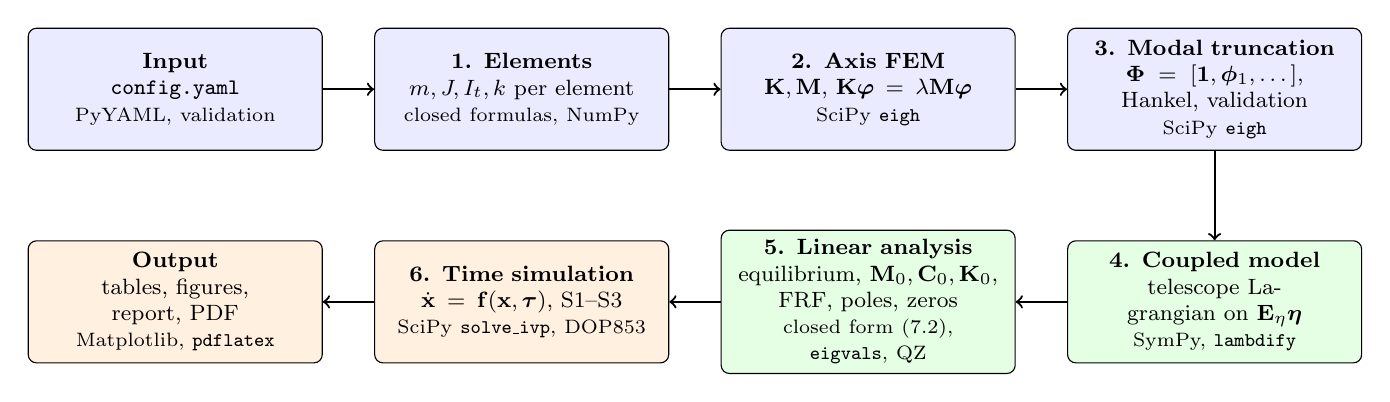
\begin{tikzpicture}[box/.style={draw, rounded corners=3pt, fill=blue!8, text width=3.5cm, align=center, minimum height=1.55cm, font=\footnotesize},box2/.style={draw, rounded corners=3pt, fill=green!10, text width=3.5cm, align=center, minimum height=1.55cm, font=\footnotesize},box3/.style={draw, rounded corners=3pt, fill=orange!12, text width=3.5cm, align=center, minimum height=1.55cm, font=\footnotesize}]
\node[box] (cfg) at (0,0) {\textbf{Input}\\ \texttt{config.yaml}\\ \scriptsize PyYAML, validation};
\node[box] (s1) at (4.4,0) {\textbf{1. Elements}\\ $m, J, I_t, k$ per element\\ \scriptsize closed formulas, NumPy};
\node[box] (s2) at (8.8,0) {\textbf{2. Axis FEM}\\ $\mathbf K,\mathbf M$, $\mathbf K\boldsymbol\varphi = \lambda\mathbf M\boldsymbol\varphi$\\ \scriptsize SciPy \texttt{eigh}};
\node[box] (s3) at (13.2,0) {\textbf{3. Modal truncation}\\ $\boldsymbol\Phi = [\mathbf 1,\boldsymbol\phi_1,\dots]$, Hankel, validation\\ \scriptsize SciPy \texttt{eigh}};
\node[box2] (s4) at (13.2,-2.7) {\textbf{4. Coupled model}\\ telescope Lagrangian on $\mathbf E_\eta\boldsymbol\eta$\\ \scriptsize SymPy, \texttt{lambdify}};
\node[box2] (s5) at (8.8,-2.7) {\textbf{5. Linear analysis}\\ equilibrium, $\mathbf M_0,\mathbf C_0,\mathbf K_0$, FRF, poles, zeros\\ \scriptsize closed form (7.2), \texttt{eigvals}, QZ};
\node[box3] (s6) at (4.4,-2.7) {\textbf{6. Time simulation}\\ $\dot{\mathbf x} = \mathbf f(\mathbf x,\boldsymbol\tau)$, S1--S3\\ \scriptsize SciPy \texttt{solve\_ivp}, DOP853};
\node[box3] (out) at (0,-2.7) {\textbf{Output}\\ tables, figures, report, PDF\\ \scriptsize Matplotlib, \texttt{pdflatex}};
\draw[->, thick] (cfg) -- (s1); \draw[->, thick] (s1) -- (s2); \draw[->, thick] (s2) -- (s3);
\draw[->, thick] (s3) -- (s4); \draw[->, thick] (s4) -- (s5); \draw[->, thick] (s5) -- (s6);
\draw[->, thick] (s6) -- (out);
\end{tikzpicture}}
\caption{Computational workflow. Blue: structural stages (Sections~\ref{sec:elements}--\ref{sec:eigen} and~\ref{sec:modal}); green: coupled model and its analysis; orange: simulation and output.}\label{fig:flow}\end{figure}
\begin{table}[H]\centering\small
\caption{Equations solved at each stage and numerical tools.}\label{tab:stages}
\begin{tabular}{p{0.04\linewidth}p{0.4\linewidth}p{0.46\linewidth}}\toprule
& equations & tool \\ \midrule
1 & $m, J, I_t, J_p$ of every layer; $k_s$ in parallel, $1/k_e$ in series (Section~\ref{sec:elements}) & closed formulas in NumPy \\
2 & assembly of $\mathbf K,\mathbf M^{\ell},\mathbf M^{c}$; $\mathbf K\boldsymbol\varphi = \lambda\mathbf M\boldsymbol\varphi$ (Section~\ref{sec:eigen}) & \texttt{scipy.linalg.eigh} (LAPACK \texttt{dsygvd}) \\
3 & $(\mathbf K - \omega^2\bar{\mathbf M})\boldsymbol\phi = \mathbf 0$ of the full FEM; Hankel norms; validation against the full model (Section~\ref{sec:modal}) & \texttt{scipy.linalg.eigh}, \texttt{numpy.linalg.solve} \\
4 & Lagrange's equations of the telescope, \eqref{eq:modal_eom} (this section) & SymPy for the derivation; \texttt{lambdify} to NumPy functions \\
5 & steady state $\mathbf r(\mathbf q_0) = \mathbf E\boldsymbol\tau_0$; Jacobians; $\mathbf G(j\omega)$; poles; zeros & NumPy \texttt{solve}, \texttt{eigvals}; SymPy \texttt{jacobian}; \texttt{scipy.linalg.eig} (QZ) \\
6 & $\dot{\mathbf x} = \mathbf f(\mathbf x,\boldsymbol\tau)$ and its linearisation & \texttt{scipy.integrate.solve\_ivp}, method DOP853 \\
7 & tables (CSV), figures, \texttt{.npz}/\texttt{.mat}/JSON exports, this document & Matplotlib, \texttt{scipy.io.savemat}, \texttt{pdflatex} \\ \bottomrule
\end{tabular}\end{table}
\subsection{Equations of the reduced model}
The default model has $n = 8$ modal coordinates $\boldsymbol\eta$ (Section~\ref{sec:modal}) and obeys \eqref{eq:modal_eom}. Its mass matrix
\begin{gather}
\mathbf M(\boldsymbol\eta) = \tilde{\mathbf M} + \mathbf E_\eta^{\mathsf T}\bigl[\mathbf M_p(\theta_p) - \bar{\mathbf M}_p\bigr]\mathbf E_\eta,\qquad \theta_p = \mathbf c_P^{\mathsf T}\boldsymbol\eta_\theta,
\end{gather}
depends on the state only through $\theta_p$, and the force vector is $\tilde{\mathbf D}\dot{\boldsymbol\eta} + \tilde{\mathbf K}\boldsymbol\eta + \mathbf E_\eta^{\mathsf T}(\mathbf C_p\dot{\mathbf q}_p + \mathbf g_p)$. The $2\times2$ payload blocks $\mathbf M_p$, $\mathbf C_p\dot{\mathbf q}_p$ and $\mathbf g_p$ of Section~\ref{sec:coupled} are derived once by SymPy (which also checks them against Lagrange's equations of $T_p - V_g$) and compiled with \texttt{lambdify}; the structural matrices are constant projections $\mathbf T^{\mathsf T}\mathbf M\mathbf T$, $\mathbf T^{\mathsf T}\mathbf K\mathbf T$, $\mathbf T^{\mathsf T}\mathbf C\mathbf T$ of the full FEM. In first-order form, with $\mathbf x = [\boldsymbol\eta,\ \dot{\boldsymbol\eta}]$,
\begin{gather}
\dot{\mathbf x} = \mathbf f(\mathbf x,\boldsymbol\tau) = \begin{bmatrix}\dot{\boldsymbol\eta}\\ \mathbf M(\boldsymbol\eta)^{-1}\Bigl[\boldsymbol\Phi^{\mathsf T}\mathbf B\boldsymbol\tau - \tilde{\mathbf D}\dot{\boldsymbol\eta} - \tilde{\mathbf K}\boldsymbol\eta - \mathbf E_\eta^{\mathsf T}(\mathbf C_p\dot{\mathbf q}_p + \mathbf g_p)\Bigr]\end{bmatrix},
\end{gather}
where the inverse is never formed: the code solves $\mathbf M\ddot{\boldsymbol\eta} = \dots$ with \texttt{numpy.linalg.solve} at every right-hand-side call. The same code, with the identity as basis, is the full-DOF reference model used for validation.
\subsection{Operating point and linearisation}
An operating point is a steady tracking motion: $\theta_p = \theta_0$, rigid azimuth rotation at $\Omega_0$ ($\dot\eta_{\psi0} = \Omega_0$, all other velocities zero), $\ddot{\boldsymbol\eta} = \mathbf 0$ and $\psi_e = 0$ (cyclic). With $\theta_p$ fixed the residual is affine in $\boldsymbol\eta$, so the static deformation and the nominal torques solve the square linear system
\begin{gather}
\begin{bmatrix}\tilde{\mathbf K} & -\boldsymbol\Phi^{\mathsf T}\mathbf B\\ \hat{\mathbf c}_P^{\mathsf T} & \mathbf 0\\ \hat{\mathbf c}_e^{\mathsf T} & \mathbf 0\end{bmatrix}\begin{bmatrix}\boldsymbol\eta_0\\ \boldsymbol\tau_0\end{bmatrix} = \begin{bmatrix}-\mathbf r_0\\ \theta_0\\ 0\end{bmatrix},
\end{gather}
with $\mathbf r_0$ the payload and bearing forces of the steady motion, solved by \texttt{numpy.linalg.solve}; the code verifies that the residual is below $10^{-8}$ of its scale. The linear matrices are the closed form of Section~\ref{sec:modal}, with the payload Jacobians of Section~\ref{sec:linear}; the test suite checks them against finite differences of the nonlinear residual. The linear model is
\begin{gather}
\mathbf M_0\,\delta\ddot{\boldsymbol\eta} + \mathbf C_0\,\delta\dot{\boldsymbol\eta} + \mathbf K_0\,\delta\boldsymbol\eta = \boldsymbol\Phi^{\mathsf T}\mathbf B\,\delta\boldsymbol\tau,\qquad \delta\dot{\mathbf x} = \mathbf A\,\delta\mathbf x + \mathbf B\,\delta\boldsymbol\tau,\qquad \mathbf y = \mathbf C_q\,\delta\boldsymbol\eta,
\end{gather}
with outputs $\psi_e, \theta_e$ (encoders), $\psi_m, \theta_m$ (motors), $\psi_L, \theta_p$ (true pointing), $\theta_r$ and the measurement errors $\psi_e - \psi_L$, $\theta_e - \theta_p$, all obtained from the rows of the modal basis at the corresponding nodes. Frequency responses, poles and zeros of this model are computed as in Section~\ref{sec:eigen}.
\subsection{Time-domain simulation}
Three scenarios are run on the default reduced model, the modal truncation of Section~\ref{sec:modal} with a single $\theta_{ref}$ (\texttt{reduction.modal.theta\_ref\_deg}), for which \eqref{eq:modal_eom} is exact for any $\theta_p$ (Table~\ref{tab:sim}). In S1 and S2 the system starts from the equilibrium of the operating point with the nominal torque applied as a feedforward, so that the perturbation is only the doublet
\begin{gather}
\tau_\psi(t) = \tau_{\psi0} + a\,\bigl[\,\chi_{[t_i,\,t_i+T)}(t) - \chi_{[t_i+T,\,t_i+2T)}(t)\,\bigr],\qquad a = 0.05\ \text{N\,m},\ T = 20\ \text{ms},\ t_i = 0.1\,T,
\end{gather}
of zero mean so that it excites the dynamics without shifting the operating point. The nonlinear system $\dot{\mathbf x} = \mathbf f(\mathbf x,\boldsymbol\tau)$ and the linear one $\delta\dot{\mathbf x} = \mathbf A\delta\mathbf x + \mathbf B\delta\boldsymbol\tau$ are integrated with the same solver and compared as $\mathbf q - \mathbf q_0$ against $\delta\mathbf q$ (the rigid drift $\Omega_0 t$ of the $\psi$'s is removed). In S3 all damping and torques are removed, the state starts from a rigid motion ($\dot\psi_i = \Omega_{max}$, $\dot\theta_i$ small, unstrained chains) and the conserved quantities $E = T + V$ and $p_\psi = \sum_i\partial\mathcal L/\partial\dot\psi_i$ are monitored.
\paragraph{Integrator.} \texttt{scipy.integrate.solve\_ivp} with method \texttt{DOP853}: an explicit Runge--Kutta scheme of order 8 (Dormand--Prince 8(5,3)) with adaptive step and embedded error control, relative tolerance $10^{-10}$ and absolute tolerance $10^{-12}$. Since the doublet is discontinuous, the integration is split at $t_i$, $t_i+T$, $t_i+2T$, so that the adaptive solver never steps across a jump (which would degrade its order). The step is limited by the highest natural frequency of the reduced chains, a few kHz, which sets the cost of a run (tens of seconds); the explicit method is adequate because the damping is light and the horizon short. The agreement is measured by $e(y) = \max_t|y_{nl}(t) - y_{lin}(t)|/\max_t|y_{lin}(t)|$ for each output.
\paragraph{Full-DOF reference.} S1 is also run on the coupled model with all FEM degrees of freedom. Its modes reach hundreds of kHz, so the explicit DOP853 step is limited by stability and the reference is integrated with relative tolerance $10^{-8}$ and absolute tolerance $10^{-10}$; the largest difference from the modal model on $\psi_e$, $\psi_m$, $\psi_L$ is $0.00035$ of the peak response.
\begin{table}[H]\centering\small
\caption{Simulation scenarios and results (relative errors of the nonlinear against the linearised response, and conservation drifts).}\label{tab:sim}
\begin{tabular}{llllp{0.4\linewidth}}\toprule
id & $\theta_0$ [deg] & $\Omega_0$ [deg/s] & forcing & result \\ \midrule
S1 & 0 & 0 & doublet on $\tau_\psi$ & $e(\psi_e) = 2.2\times10^{-7}$, $e(\psi_L) = 1.6\times10^{-10}$ \\
S2 & 0 & 10 & doublet on $\tau_\psi$ & $e(\psi_e) = 1.2\times10^{-6}$, $e(\psi_L) = 9.9\times10^{-9}$ \\
S3 & 0 & 10 & conservation, $\mathbf C = \mathbf 0$, $\boldsymbol\tau = \mathbf 0$ & $|\Delta E|/E = 1.8\times10^{-14}$, $|\Delta p_\psi|/p_\psi = 2.5\times10^{-12}$ \\
\bottomrule\end{tabular}\end{table}
In S1 the polar channels respond only through the products of inertia, so their linear response is of the same order as the quadratic term $\tfrac12 J_{\psi,p}'\dot\psi^2$ that the linearisation drops: their relative error is therefore not an index of the quality of the linearisation, and only the azimuth channels are used for it. Their amplitude (about $10^{-12}$\,rad) is also comparable with the absolute tolerance of the integrator, so the isolated spikes visible on the nonlinear polar curves are integration noise, not dynamics.
\begin{figure}[H]\centering
\includegraphics[width=0.9\linewidth,height=0.45\textheight,keepaspectratio]{../figures/simulazione_S1.pdf}
\caption{S1: nonlinear (solid) and linearised (dashed) response to the $\tau_\psi$ doublet at $\Omega_0 = 0$. \emph{Result from placeholder parameters.}}\end{figure}
\begin{figure}[H]\centering
\includegraphics[width=0.9\linewidth,height=0.45\textheight,keepaspectratio]{../figures/simulazione_S2.pdf}
\caption{S2: the same doublet while tracking at $\Omega_{max}$; the cross response on $\theta_e$ and $\theta_p$ is the gyroscopic coupling. \emph{Result from placeholder parameters.}}\end{figure}
\begin{figure}[H]\centering
\includegraphics[width=0.9\linewidth,height=0.45\textheight,keepaspectratio]{../figures/simulazione_S3.pdf}
\caption{S3: drift of $E = T + V$ and $p_\psi$ in the conservative case. \emph{Result from placeholder parameters.}}\end{figure}
\subsection{Software}
\begin{table}[H]\centering\small
\caption{Software used to produce this document.}\label{tab:software}
\begin{tabular}{ll}\toprule
Python & 3.12.3 \\
NumPy & 2.5.4 \\
SciPy & 1.18.1 (LAPACK through \texttt{scipy.linalg}) \\
SymPy & 1.14.0 \\
Matplotlib, PyYAML, pytest & figures, input parsing, test suite \\
\texttt{pdflatex} & this document (TikZ for the drawings) \\ \bottomrule
\end{tabular}\end{table}
All results are reproducible with \texttt{python run\_all.py}; the symbolic derivation is deterministic and the numerical tolerances above are fixed in \texttt{simulate.py}.
\section{Assumptions and placeholders}\label{sec:assumptions}
\begin{longtable}{p{0.31\linewidth}p{0.12\linewidth}p{0.49\linewidth}}
\toprule code & status & description \\ \midrule\endhead
\texttt{Q6\_MATERIALI} & placeholder & Q6: placeholder materials ['steel', 'aluminium'] (steel: rho = 8000 kg/m\^{}3, G = 77 GPa, aluminium: rho = 2810 kg/m\^{}3, G = 26.9 GPa). \\
\texttt{TELESCOPIO\_SENZA\_ALBERO} & note & Polar element 3 in mode: telescope: no shaft under the telescope. In the hub model its nodes 3 and 4 coincide with the hub centre H; the telescope is the node P attached to H by k\_b, and its inertia enters only through the payload section. \\
\texttt{MOZZO\_TELESCOPIO} & note & Hub model (polar.hub.enabled: true): the hub (two side hubs, tube + flange, and the support ring) replaces polar elements [2, 4] and its centre H takes the nodes of element 3; the telescope is a node P off the chain, attached to H by k\_b = 9800 N m/rad. \\
\texttt{MOZZO\_K\_B} & placeholder & k\_b = 9800 N m/rad (telescope to hub) is a placeholder (placeholder: two-mass estimate from the antiresonance (18.1 Hz) and resonance (\textasciitilde{}48 Hz) measured at the elevation encoder): it sets the antiresonance at the encoder. \\
\texttt{MOZZO\_INERZIA\_AZIMUT} & placeholder & hub.inertia.in\_azimuth\_load = false: the inertia of the hub about z\_hat is added to J\^{}ax. Check whether the azimuth load exported from Onshape already contains the hub parts. \\
\texttt{NODI\_SENZA\_INERZIA\_AZIMUT} & placeholder & Azimuth axis: no concentrated inertia at encoder (node 1), motor (node 5) (rotor/disc missing): those nodes carry only the shaft mass and are almost inertia-free. This affects the zeros and the high modes (typically strongly) and the choice of the truncation modes. \\
\texttt{Q5\_GIUNZIONI\_AZIMUT} & placeholder & Q5: azimuth axis without joint compliances (shrink fits, keys, flanges): the stiffnesses are those of the shafts alone and probably overestimate the real one. \\
\texttt{Q8\_CUSCINETTI\_AZIMUT} & placeholder & Q8: zero viscous bearing friction on the azimuth axis. \\
\texttt{NODI\_SENZA\_INERZIA\_POLARE} & placeholder & Polar axis: no concentrated inertia at encoder (node 1), motor (node 7) (node\_inertias entirely commented out): those nodes carry only the shaft mass and are almost inertia-free. This affects the zeros and the high modes (typically strongly) and the choice of the truncation modes. \\
\texttt{Q5\_GIUNZIONI\_POLARE} & placeholder & Q5: polar axis without joint compliances (shrink fits, keys, flanges): the stiffnesses are those of the shafts alone and probably overestimate the real one. \\
\texttt{Q7\_POSIZIONE\_POLARE} & note & Q7: y\_node1\_from\_o2\_mm = null. The contribution of the polar shaft to the azimuth inertia (J\^{}ax) is computed from the transverse moments of the parts about their own centres only, without Steiner terms about o\_2. Irrelevant: the azimuth load includes the polar shafts (includes\_polar\_shafts: true), so J\^{}ax is not added. \\
\texttt{Q8\_CUSCINETTI\_POLARE} & placeholder & Q8: zero viscous bearing friction on the polar axis. \\
\texttt{TERNE\_ORIGINI} & note & Origins on z\_hat: dist(O\_N, o\_1) = 59.695 mm, dist(O\_N, o\_2) = 548.865 mm (o\_2 = centre of rotation of the polar shaft). O\_N is the origin of the Onshape assembly (centre of the base of the azimuth shaft) and x\_hat, y\_hat, z\_hat are its axes. \\
\texttt{RIDUZIONE\_MODALE} & note & Reduction: Gawronski modal truncation of the full FEM of each axis (band 2000 Hz, cut-off 4000 Hz, static correction: none). \\
\texttt{Q8\_SMORZAMENTO} & placeholder & Q8: stiffness-proportional damping, C = beta K, with zeta = 0.01 on the first flexible mode of each axis. Placeholder: the height of the FRF peaks and notches is not representative. \\
\texttt{Q11\_OMEGA\_MAX} & placeholder & Q11: tracking rates [0.0, 10.0] deg/s; Omega\_max = 10 deg/s placeholder. It sets the gyroscopic coupling. \\
\texttt{Q12\_FORCELLA\_RIGIDA} & note & Q12: rigid fork between azimuth node 9 and the polar bearings. The reaction of tau\_theta does no work on psi\_L (section 9.4). \\
\texttt{MISURA\_THETA0\_3} & placeholder & Elevation\_BodeMeasurement\_bode\_New\_16\_10\_26.csv: elevation during the test not recorded in the file; theta0 = 0 deg assumed. \\
\texttt{MISURE\_SPERIMENTALI} & note & Comparison with 5 plant measurements (Kollmorgen WorkBench, LucyIdentification); K\_t = 0.258 N m/A. The Validation folder is not used. \\
\texttt{JAX\_NEL\_CARICO} & note & The azimuth load 'load (fork + polar shafts)' (node 9) includes the polar shafts (includes\_polar\_shafts: true): J\^{}ax = 8.3476e-04 kg m\^{}2 computed from the polar elements is not added, because their moment about the azimuth axis, with the real distances from the axis, is already in the CAD value. \\
\texttt{PAYLOAD\_SEGNO\_PRODOTTI} & placeholder & payload.products\_sign = 'tensor': the sign convention of the Onshape products of inertia is not verified on a test body; it affects the products I\_IJ, I\_IK, I\_JK, not the diagonal moments. \\
\texttt{Q3\_TELESCOPIO} & note & Q3: telescope from the tensor entered in config.yaml (frame: cad\_cg, Onshape, Telescopio LAMERA <1>, without mate connector), without subtractions (subtract\_shaft\_parts: false): the tensor must contain the telescope only, not the parts of the polar axis already modelled in the elements. \\
\bottomrule\end{longtable}
\end{document}